% =====================================================================
%  Vision & Multimodal AI Engineer --- The Memorize-Cold Sheet
%  Comprehensive reference on Computer Vision, CNNs, ViTs, Detection,
%  Segmentation, SSL, VLMs, Diffusion, Video, 3DGS, and Vision Systems
%  Compile: pdflatex main.tex (twice, for the table of contents)
% =====================================================================
\documentclass[8pt,twocolumn,a4paper]{extarticle}

% ---------- page ----------
\usepackage[a4paper,top=13mm,bottom=13mm,left=11mm,right=11mm,columnsep=6mm,headsep=3mm,footskip=6mm]{geometry}
\setlength{\columnseprule}{0.2pt}

% ---------- fonts ----------
\usepackage[T1]{fontenc}
\usepackage[sc]{mathpazo}
\linespread{1.04}
\usepackage[scaled=0.90]{helvet}
\renewcommand{\ttdefault}{lmtt}
\usepackage{microtype}

% ---------- maths, tables ----------
\usepackage{amsmath,amssymb,bm}
\usepackage{booktabs,tabularx,array,multirow}
\usepackage{enumitem}
\setlist{nosep,leftmargin=1.1em,labelsep=0.4em}
\setlist[itemize]{label={\color{acc}\tiny$\blacktriangleright$}}
\renewcommand{\arraystretch}{1.12}
\setlength{\tabcolsep}{3pt}

% ---------- colour ----------
\usepackage[dvipsnames]{xcolor}
\definecolor{acc}{HTML}{144D78}   % deep maritime blue
\definecolor{acc2}{HTML}{B84A29}  % terracotta / rust
\definecolor{acc3}{HTML}{1E754C}  % emerald green
\definecolor{ink}{HTML}{222222}
\definecolor{soft}{HTML}{F3F6FA}
\definecolor{soft2}{HTML}{FBF4EE}
\definecolor{rule}{HTML}{9DB3C8}
\definecolor{mute}{HTML}{6B7785}
\color{ink}

% ---------- diagrams ----------
\usepackage{tikz}
\usetikzlibrary{arrows.meta,positioning,calc,fit,shapes.geometric,backgrounds,decorations.pathreplacing,matrix}
\usepackage{pgfplots}
\pgfplotsset{compat=1.16}
\tikzset{
  >={Stealth[length=1.6mm]},
  box/.style={draw=acc,rounded corners=1pt,line width=0.5pt,inner sep=2pt,minimum height=4.2mm,font=\scriptsize,align=center,fill=white},
  sbox/.style={box,fill=soft},
  hbox/.style={box,draw=acc2,fill=soft2},
  gbox/.style={box,draw=acc3,fill=acc3!8},
  lab/.style={font=\scriptsize\color{mute},align=center},
  arr/.style={->,draw=acc,line width=0.5pt},
  darr/.style={->,draw=acc2,line width=0.5pt,dashed},
}

% ---------- boxes ----------
\usepackage[most]{tcolorbox}
\tcbset{
  base/.style={enhanced,breakable,boxrule=0pt,arc=0pt,outer arc=0pt,
    left=3pt,right=3pt,top=2pt,bottom=2pt,before skip=3pt,after skip=4pt,
    fonttitle=\sffamily\bfseries\scriptsize,coltitle=white,
    toptitle=0.5pt,bottomtitle=0.5pt,lefttitle=3pt},
}
% Interview Q&A block
\newtcolorbox{qa}[1][]{base,colback=soft,borderline west={1.6pt}{0pt}{acc},
  before upper={{\sffamily\bfseries\scriptsize\color{acc}INTERVIEW Q\&A\enspace{\color{mute}\textbar}\enspace\MakeUppercase{#1}}\par\smallskip}}
% Must-memorize facts
\newtcolorbox{mem}[1][Memorize]{base,colback=soft2,borderline west={1.6pt}{0pt}{acc2},
  before upper={{\sffamily\bfseries\scriptsize\color{acc2}\MakeUppercase{#1}}\par\smallskip}}
% Traps
\newtcolorbox{trap}[1][Traps]{base,colback=white,borderline west={1.6pt}{0pt}{acc3},
  before upper={{\sffamily\bfseries\scriptsize\color{acc3}\MakeUppercase{#1}}\par\smallskip}}

% One question/answer pair
\newcounter{qn}
\newcommand{\Q}[2]{\refstepcounter{qn}%
  \par\noindent{\sffamily\bfseries\color{acc}Q\theqn.}~{\bfseries #1}\par
  \noindent\hangindent=0.9em\hangafter=0{#2}\par\vspace{2.2pt}}
% Rapid-fire single line
\newcommand{\RF}[2]{\par\noindent\hangindent=0.9em\hangafter=1{\bfseries #1}\;{\color{mute}$\to$}\;#2\par}

% ---------- headings ----------
\usepackage{titlesec}
\titleformat{\section}{\sffamily\bfseries\large\color{acc}}{\thesection}{0.5em}{}[{\color{acc}\titlerule[0.6pt]}]
\titlespacing*{\section}{0pt}{6pt}{3pt}
\titleformat{\subsection}{\sffamily\bfseries\normalsize\color{acc}}{\thesubsection}{0.45em}{}
\titlespacing*{\subsection}{0pt}{4pt}{1.5pt}
\titleformat{\paragraph}{\sffamily\bfseries\small\color{acc2}}{}{0pt}{}
\titlespacing*{\paragraph}{0pt}{2pt}{1pt}
\setcounter{secnumdepth}{2}

% ---------- header / footer ----------
\usepackage{fancyhdr}
\pagestyle{fancy}
\fancyhf{}
\renewcommand{\headrulewidth}{0.3pt}
\renewcommand{\headrule}{{\color{rule}\hrule width\headwidth height\headrulewidth}}
\fancyhead[L]{\sffamily\scriptsize\color{mute}Vision \& Multimodal AI Engineer --- memorize-cold sheet}
\fancyhead[R]{\sffamily\scriptsize\color{mute}\nouppercase{\leftmark}}
\fancyfoot[C]{\sffamily\scriptsize\color{mute}\thepage}
\renewcommand{\sectionmark}[1]{\markboth{\thesection\ \ #1}{}}

\usepackage[hidelinks]{hyperref}
\hypersetup{pdftitle={Vision and Multimodal AI Engineer: memorize-cold sheet},pdfauthor={Achilles}}
\usepackage{xurl}
\usepackage{listings}
\usepackage{needspace}
\lstset{language=Python,basicstyle=\ttfamily\fontsize{6.6}{7.6}\selectfont,keywordstyle=\color{acc}\bfseries,commentstyle=\color{mute}\itshape,stringstyle=\color{acc2},backgroundcolor=\color{soft},frame=leftline,framerule=1.2pt,rulecolor=\color{acc},xleftmargin=4pt,framexleftmargin=3pt,aboveskip=2pt,belowskip=3pt,columns=fullflexible,keepspaces=true,showstringspaces=false,breaklines=true}

% ---------- small helpers ----------
\newcommand{\tb}[1]{\textbf{#1}}
\newcommand{\hl}[1]{{\color{acc2}\textbf{#1}}}
\newcommand{\ra}{\,{\color{mute}$\rightarrow$}\,}
\newcommand{\lab}[1]{{\color{mute}\scriptsize[#1]}}
\newcommand{\cn}[1]{{\color{mute}\,[#1]}}
\newcolumntype{L}{>{\raggedright\arraybackslash}X}
\renewcommand{\tabularxcolumn}[1]{>{\raggedright\arraybackslash}p{#1}}
\usepackage[export]{adjustbox}
\usepackage{etoolbox}
% never leave a section heading stranded at the bottom of a column
\pretocmd{\section}{\needspace{16\baselineskip}}{}{}
\pretocmd{\subsection}{\needspace{6\baselineskip}}{}{}
\raggedbottom % no stretched glue gaps inside columns
% keep a box title together with its first lines
\BeforeBeginEnvironment{mem}{\needspace{14\baselineskip}}
\BeforeBeginEnvironment{qa}{\needspace{7\baselineskip}}
\BeforeBeginEnvironment{trap}{\needspace{5\baselineskip}}
% Section opener: diagram beside its explanation when the diagram is narrow,
% diagram on top at full column width when it is wide (keeps labels legible).
\newsavebox{\dgbox}
\newlength{\dgw}
\newcommand{\diagpair}[2]{%
  \par\sbox{\dgbox}{#1}%
  \ifdim\wd\dgbox>0.47\columnwidth
    \begin{center}\adjustbox{max width=\columnwidth}{\usebox{\dgbox}}\end{center}\vspace{-3pt}
    {\small #2\par}\vspace{2pt}%
  \else
    \setlength{\dgw}{\wd\dgbox}%
    \noindent\begin{minipage}[t]{\dgw}\vspace{0pt}\usebox{\dgbox}\end{minipage}\hfill
    \begin{minipage}[t]{\dimexpr\columnwidth-\dgw-3mm\relax}\vspace{1pt}\small #2\end{minipage}\par\vspace{2pt}%
  \fi}
\newcommand{\tsmall}{\scriptsize}

\begin{document}
\twocolumn[{%
\begin{tikzpicture}[remember picture,overlay]
\fill[acc] ($(current page.north west)+(0,-0mm)$) rectangle ($(current page.north east)+(0,-4mm)$);
\end{tikzpicture}
\vspace*{1mm}
{\sffamily\bfseries\fontsize{19}{21}\selectfont\color{acc}Vision \& Multimodal AI Engineer}\\[1mm]
{\sffamily\large\color{acc2}The memorize-cold sheet: what you must be able to answer in your sleep}\\[1.5mm]
{\small\color{mute}Built across the entire visual AI stack: geometry, classical filtering, CNNs, ViTs, object detection, segmentation, SSL, CLIP, modern VLMs, diffusion, flow matching, video foundation models, 3DGS, and edge vision systems. Interview Q\&A first, derivations only where the answer \emph{is} the derivation. Snapshot: October 2026.}
\vspace{2mm}
{\color{rule}\hrule height 0.4pt}
\vspace{3mm}
}]
\thispagestyle{plain}

\section*{How to use this sheet}
\begin{itemize}
\item \textbf{Three passes.} Day 1: read a section. Day 3: cover every answer and state the math, mechanics, and trade-offs out loud. Day 7 and 21: drill only missed items.
\item \textbf{Boxes.} {\color{acc}\textbf{Blue}} = interview Q\&A. {\color{acc2}\textbf{Rust}} = numbers, formulas, and invariants to memorize. {\color{acc3}\textbf{Green}} = traps interviewers use to catch out candidates who memorize buzzwords without understanding the physics.
\item \textbf{The five numbers of any vision model}: $H\times W$ (resolution), $C$ (channels / embedding dimension), $P$ (patch size / stride), $L$ (layers / depth), and $N_{\text{tok}}$ (visual tokens). FLOPs, receptive field, memory, and latency all follow.
\item \textbf{Answer shape}: mechanism \ra\ number \ra\ trade-off \ra\ what you would measure and debug.
\item \textbf{FLOPs vs MACs.} $1$ MAC $= 2$ FLOPs. Conv formulas here count FLOPs ($2\times$); transformer formulas follow the Swin/ViT papers and count MACs ($4ND^2 + 2N^2D$ per attention layer). Say which one you mean in an interview.
\end{itemize}

\begin{mem}[The 12 numbers everyone asks in Vision]
\begin{tabularx}{\linewidth}{@{}lL@{}}
$2 C_{\text{in}} C_{\text{out}} K^2 H W$ & FLOPs of a 2D convolution ($H, W$ output spatial size)\\
$\frac{H W}{P^2}$ & Visual tokens for an image in ViT ($P=14 \implies 256$ for $224^2$)\\
$25.6\text{M} / 4.1\text{G}$ & ResNet-50 parameters and FLOPs at $224\times 224$\\
$86\text{M} / 307\text{M}$ & ViT-B/16 and ViT-L/16 parameters ($17.6 / 61.6$ GMACs at $224^2$)\\
$8\times$ & Spatial compression factor of standard SD / Flux VAEs ($512^2 \to 64^2$)\\
$\tau \approx 0.07$ & CLIP initial temperature ($1/\tau \approx 14$); learned logit scale clamped at $100$\\
$59\text{ floats}$ & One 3D Gaussian: pos 3, quat 4, scale 3, opacity 1, SH 48 $= 236$ B in FP32\\
$632\text{M}$ & SAM (Segment Anything) ViT-H image encoder parameter count\\
$0.18215$ & SD 1.x VAE latent scale factor (SDXL: $0.13025$); forget it and samples are grey mush\\
$\text{IoU} \ge 0.5$ & Standard VOC/PASCAL positive detection match threshold\\
$RF_l = RF_{l-1} + (K-1)J$ & Cumulative receptive field recurrence relation\\
$33.3\text{ ms}$ & Real-time camera streaming latency budget at 30 FPS\\
\end{tabularx}
\end{mem}

{\small\tableofcontents}

\section{Geometry, Projection \& Classical Vision}\label{sec:geom}
\lab{epipolar geometry \textperiodcentered\ pinhole optics \textperiodcentered\ feature detectors \textperiodcentered\ filtering \textperiodcentered\ optical flow}

\noindent\begin{minipage}[t]{0.44\columnwidth}\vspace{0pt}\centering
\resizebox{\linewidth}{!}{%
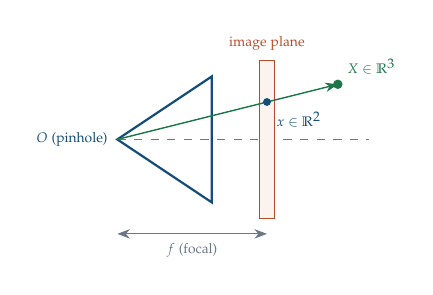
\begin{tikzpicture}[x=1mm,y=1mm,every node/.style={font=\tiny}]
\draw[draw=acc,thick] (0,0) -- (12,8) -- (12,-8) -- cycle;
\node[acc,left] at (0,0) {$O$ (pinhole)};
\draw[draw=mute,dashed] (0,0) -- (32,0);
\draw[draw=acc2,fill=soft2] (18,-10) rectangle (20,10);
\node[acc2,above] at (19,10) {image plane};
\draw[arr,acc3] (0,0) -- (28,7);
\fill[acc3] (28,7) circle (0.6mm) node[above right] {$X \in \mathbb{R}^3$};
\fill[acc] (19,4.75) circle (0.5mm) node[below right] {$x \in \mathbb{R}^2$};
\draw[<->,mute] (0,-12) -- (19,-12) node[midway,below] {$f$ (focal)};
\end{tikzpicture}%
}
\end{minipage}\hfill
\begin{minipage}[t]{0.54\columnwidth}\vspace{1pt}\small
\textbf{World to pixel coordinates.} 3D world point $\mathbf{X}_w = [X, Y, Z, 1]^\top$ maps to 2D homogeneous pixel $\mathbf{x} = [u, v, 1]^\top$ via:
$$\lambda \begin{bmatrix} u \\ v \\ 1 \end{bmatrix} = \mathbf{K} [\mathbf{R} \mid \mathbf{t}] \begin{bmatrix} X \\ Y \\ Z \\ 1 \end{bmatrix}$$
where $\mathbf{K}$ is the $3\times 3$ intrinsic matrix, $\mathbf{R} \in SO(3)$ is rotation, and $\mathbf{t} \in \mathbb{R}^3$ is translation.\\[2pt]
{\color{acc2}$\blacktriangleright$} Intrinsic matrix: $f_x, f_y$ focal lengths, $c_x, c_y$ principal point, $s$ skew.\\
{\color{acc2}$\blacktriangleright$} Depth ambiguity: $\lambda = Z_c$ is lost in projection.
\end{minipage}

\begin{mem}[Epipolar Geometry \& Core Transformations]
Two calibrated cameras observing scene point $X$ have image coordinates $x, x'$.
\begin{itemize}
\item \textbf{Essential Matrix} $\mathbf{E} = [\mathbf{t}]_\times \mathbf{R} \in \mathbb{R}^{3\times 3}$: relates normalized camera coordinates: $x'^\top \mathbf{E} x = 0$. $\mathbf{E}$ has 5 degrees of freedom (two equal singular values, one zero).
\item \textbf{Fundamental Matrix} $\mathbf{F} = \mathbf{K}'^{-\top} \mathbf{E} \mathbf{K}^{-1}$: relates uncalibrated pixel coordinates: $x'^\top \mathbf{F} x = 0$. $\mathbf{F}$ has rank 2, 7 degrees of freedom. Epipolar line $l' = \mathbf{F} x$. Epipoles satisfy $\mathbf{F} e = 0, \mathbf{F}^\top e' = 0$.
\item \textbf{Normalized 8-Point Algorithm}: Hartley's algorithm translates point centroid to $(0,0)$ and scales average distance to $\sqrt{2}$ before constructing matrix $A f = 0$. Enforces $\det(\mathbf{F})=0$ by zeroing smallest singular value in SVD.
\item \textbf{Homography} $\mathbf{H} \in \mathbb{R}^{3\times 3}$: maps coplanar 3D points between two views: $x' \sim \mathbf{H} x$. Solved with 4 point pairs using Direct Linear Transformation (DLT) + RANSAC.
\end{itemize}
\end{mem}

\begin{qa}[Classical Features, Edges \& Keypoints]
\Q{Walk through the 4 stages of Canny edge detection in detail.}{
\textbf{1. Gaussian smoothing}: Convolve image with Gaussian filter ($G_\sigma, \sigma \approx 1.4$) to suppress high-frequency sensor noise.
\textbf{2. Gradient calculation}: Apply Sobel operators $G_x = \begin{bmatrix}-1&0&1\\-2&0&2\\-1&0&1\end{bmatrix}, G_y = G_x^\top$ to compute gradient magnitude $|G| = \sqrt{G_x^2 + G_y^2}$ and direction $\theta = \arctan(G_y / G_x)$. Quantize $\theta$ into 4 canonical sectors: $0^\circ, 45^\circ, 90^\circ, 135^\circ$.
\textbf{3. Non-Maximum Suppression (NMS)}: Thin wide edges down to 1-pixel ridges. At each pixel, compare $|G|$ with its two neighbors along direction $\theta$. If $|G|$ is smaller than either neighbor, suppress it to 0.
\textbf{4. Double thresholding \& Hysteresis}: Define high threshold $T_{\text{high}}$ and low threshold $T_{\text{low}}$ ($T_{\text{high}} \approx 2-3\times T_{\text{low}}$). Pixels with $|G| \ge T_{\text{high}}$ are marked as strong edges; pixels with $T_{\text{low}} \le |G| < T_{\text{high}}$ are weak edges. Retain weak edges \emph{only} if connected to a strong edge via 8-connectivity.}
\Q{How does the Harris Corner Detector mathematically separate corners, edges, and flats?}{
Compute second moment matrix $M = \sum_{(u,v)} w(u,v) \begin{bmatrix} I_x^2 & I_x I_y \\ I_x I_y & I_y^2 \end{bmatrix}$, where $w(u,v)$ is a Gaussian window.
The eigenvalues $\lambda_1, \lambda_2$ of $M$ characterize the local intensity curvature:
\begin{itemize}
\item \textbf{Flat region}: $\lambda_1 \approx 0, \lambda_2 \approx 0$ (no intensity variation).
\item \textbf{Edge}: $\lambda_1 \gg \lambda_2 \approx 0$ (variation along gradient normal, invariant along tangent).
\item \textbf{Corner}: $\lambda_1, \lambda_2$ both large (variation in all directions).
\end{itemize}
Harris avoids explicit eigendecomposition by defining corner response $R$:
$$R = \det(M) - k \cdot (\text{Tr}(M))^2 = \lambda_1 \lambda_2 - k (\lambda_1 + \lambda_2)^2 \quad (k \in [0.04, 0.06])$$
$R > 0$ indicates a corner, $R < 0$ indicates an edge, and $|R| \approx 0$ indicates a flat region.}
\Q{Compare SIFT, SURF, and ORB feature extractors.}{
\textbf{SIFT (Lowe, 2004)}: Scale-space DoG (Difference of Gaussians) extrema localization; 3D quadratic sub-pixel refinement; gradient orientation histogram assignment (rotation invariance); $4\times 4$ spatial grid $\times 8$ orientation bins $= 128$-d descriptor. High accuracy, robust to illumination and 3D affine viewpoint shifts, but computationally slow.
\textbf{SURF (Bay et al., 2006)}: Replaces Gaussian second derivatives with box filters evaluated via Integral Images; Haar-wavelet responses; 64-d descriptor. $3\times$ faster than SIFT.
\textbf{ORB (Rublee et al., 2011)}: FAST corner detector with intensity centroid orientation (oFAST) $+$ steered BRIEF binary descriptors (rBRIEF). Matches descriptors via bitwise Hamming distance (XOR + popcount) on CPU. Runs $100\times$ faster than SIFT, patent-free, widely used in real-time visual SLAM.}
\Q{State the Optical Flow constraint equation and compare Lucas-Kanade vs Horn-Schunck.}{
\textbf{Brightness Constancy Assumption}: $I(x+u, y+v, t+1) = I(x, y, t)$. First-order Taylor expansion yields:
$$I_x u + I_y v + I_t = 0 \iff \nabla I \cdot \mathbf{v} + I_t = 0$$
This is 1 equation with 2 unknowns $(u, v)$ (Aperture Problem: flow parallel to edges is ambiguous).
\textbf{Lucas-Kanade}: Assumes flow is constant within a small local $n\times n$ window ($n=5$). Solves overdetermined system via least squares:
$\begin{bmatrix} u \\ v \end{bmatrix} = \left(\sum \begin{bmatrix} I_x^2 & I_x I_y \\ I_x I_y & I_y^2 \end{bmatrix}\right)^{-1} \left( -\sum \begin{bmatrix} I_x I_t \\ I_y I_t \end{bmatrix} \right)$.
Fails on large displacements (requires multi-scale image pyramids).
\textbf{Horn-Schunck}: Global variational formulation minimizing brightness error $+$ global smoothness:
$E(u, v) = \iint \left( (I_x u + I_y v + I_t)^2 + \alpha^2 (\|\nabla u\|^2 + \|\nabla v\|^2) \right) dx dy$.
Solves dense flow everywhere via Gauss-Seidel iteration, filling in smooth flow over untextured regions.}
\end{qa}

\begin{trap}[Coordinate \& Geometric Traps]
\begin{itemize}
\item \textbf{Essential vs Fundamental Matrix}: $\mathbf{E}$ operates on normalized ray coordinates $x_{\text{norm}} = \mathbf{K}^{-1} x_{\text{pix}}$ and depends purely on extrinsic pose $[R|t]$. $\mathbf{F}$ operates on raw pixel coordinates and absorbs camera intrinsics $\mathbf{K}$.
\item \textbf{Rank-2 Enforcement in Fundamental Matrix}: Raw linear estimation yields full rank-3 $\mathbf{F}$. If SVD singular values $[\sigma_1, \sigma_2, \sigma_3]$ are not forced to $[\sigma_1, \sigma_2, 0]$, epipolar lines will fail to intersect at a unique epipole.
\end{itemize}
\end{trap}

\section{Classical Vision: Keypoints, Geometry \& Flow}\label{sec:classical}
\lab{Harris corner \textperiodcentered\ SIFT \textperiodcentered\ ORB \textperiodcentered\ RANSAC \textperiodcentered\ Essential/Fundamental \textperiodcentered\ Lucas-Kanade \textperiodcentered\ RAFT}

\noindent\begin{minipage}[t]{0.42\columnwidth}\vspace{0pt}\centering
\resizebox{\linewidth}{!}{%
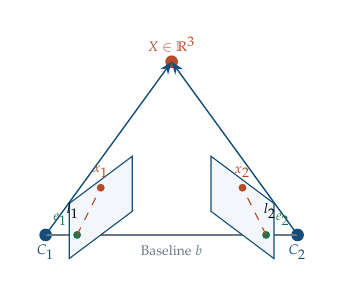
\begin{tikzpicture}[x=1mm,y=1mm,every node/.style={font=\tiny}]
% Left Camera C1
\fill[acc] (0,0) circle (0.8mm) node[below] {$C_1$};
% Right Camera C2
\fill[acc] (32,0) circle (0.8mm) node[below] {$C_2$};
\draw[mute,thick] (0,0) -- (32,0) node[midway,below] {Baseline $b$};
% 3D Point X
\fill[acc2] (16,22) circle (0.8mm) node[above] {$X \in \mathbb{R}^3$};
% Rays
\draw[arr,acc] (0,0) -- (16,22);
\draw[arr,acc] (32,0) -- (16,22);
% Image planes
\draw[draw=acc,fill=soft] (3,4) -- (11,10) -- (11,3) -- (3,-3) -- cycle;
\draw[draw=acc,fill=soft] (21,10) -- (29,4) -- (29,-3) -- (21,3) -- cycle;
% Epipoles and projected points
\fill[acc3] (4,0) circle (0.5mm) node[above left] {$e_1$};
\fill[acc3] (28,0) circle (0.5mm) node[above right] {$e_2$};
\fill[acc2] (7,6) circle (0.5mm) node[above] {$x_1$};
\fill[acc2] (25,6) circle (0.5mm) node[above] {$x_2$};
\draw[draw=acc2,dashed] (4,0) -- (7,6) node[midway,left] {$l_1$};
\draw[draw=acc2,dashed] (28,0) -- (25,6) node[midway,right] {$l_2$};
\end{tikzpicture}%
}
\end{minipage}\hfill
\begin{minipage}[t]{0.56\columnwidth}\vspace{1pt}\small
\textbf{The Epipolar Constraint.} $X, C_1, C_2$ define the epipolar plane.
Baseline $b$ pierces image planes at epipoles $e_1, e_2$. Observing point $x_1$ constrains correspondence $x_2$ to lie along epipolar line $l_2 = \mathbf{F} x_1$.\\[2pt]
{\color{acc2}$\blacktriangleright$} Calibrated: $\hat{x}_2^T \mathbf{E} \hat{x}_1 = 0$ ($5$ DoF, SVD $[\sigma, \sigma, 0]$).\\
{\color{acc2}$\blacktriangleright$} Uncalibrated: $x_2^T \mathbf{F} x_1 = 0$ ($7$ DoF, rank 2).\\
{\color{acc2}$\blacktriangleright$} Search: 2D correspondence reduced to 1D ray.
\end{minipage}

\begin{mem}[Keypoint Detectors \& Descriptors at a Glance]
\begin{tabularx}{\columnwidth}{@{}l l l X@{}}
\toprule
\textbf{Method} & \textbf{Detector} & \textbf{Descriptor} & \textbf{Properties \& Invariance} \\
\midrule
\textbf{Harris} & Structure Tensor $M$ & None & Rotation, translation; \hl{NOT} scale-invariant \\
\textbf{SIFT} & DoG Scale-Space & 128-D L2 & Scale, rotation, illumination; compute-heavy \\
\textbf{SURF} & Box filters & 64-D L2 & Fast scale-invariance via integral images \\
\textbf{FAST} & 16-px circle test & None & Ultra-fast corner detector ($\sim$0.5\,ms) \\
\textbf{ORB} & Oriented FAST & 256-bit bin & Rotation-invariant; Hamming dist (POPCNT) \\
\bottomrule
\end{tabularx}
\end{mem}

\begin{qa}[Classical Corner Detection \& Invariant Descriptors]
\Q{Derive the Harris Corner Detector response and explain why it is rotation-invariant but not scale-invariant.}{
The local auto-correlation function measures intensity variation under shift $(\Delta x, \Delta y)$:
$$E(\Delta x, \Delta y) \approx [\Delta x, \Delta y] \, M \, [\Delta x, \Delta y]^T$$
$$\text{where } M = \sum_{(x,y) \in W} w(x,y) \begin{bmatrix} I_x^2 & I_x I_y \\ I_x I_y & I_y^2 \end{bmatrix}$$
Let eigenvalues of $M$ be $\lambda_1, \lambda_2$:
\begin{itemize}
\item \textbf{Flat region}: $\lambda_1 \approx 0, \lambda_2 \approx 0$.
\item \textbf{Edge}: $\lambda_1 \gg \lambda_2 \approx 0$ (or vice versa).
\item \textbf{Corner}: $\lambda_1, \lambda_2 \gg 0$ (large variation in all spatial directions).
\end{itemize}
Harris avoids costly SVD eigenvalue computation using trace and determinant:
$$R = \det(M) - k \cdot (\operatorname{Tr}(M))^2 = \lambda_1 \lambda_2 - k(\lambda_1 + \lambda_2)^2$$
with $k \in [0.04, 0.06]$.
\textbf{Invariance}: Rotation transforms $M \to R M R^T$, preserving trace and determinant ($\det(R M R^T) = \det(M)$). However, scaling an image shrinks or expands features: a corner at fine scale becomes a smooth curve at coarse scale, breaking fixed window $W$.}

\Q{How does SIFT achieve scale invariance, and why does Lowe's Ratio Test reject false matches?}{
\textbf{Scale Invariance}: SIFT builds an octave scale space by convolving the image with Gaussians of increasing variance $\sigma$, then computes Difference-of-Gaussians (DoG):
$$D(x, y, \sigma) = (G(x, y, k\sigma) - G(x, y, \sigma)) * I(x, y)$$
Extrema (minima/maxima) are detected by comparing each pixel against its 8 neighbors in the current scale and $9+9=18$ neighbors in adjacent scales (26 comparisons). Sub-pixel localization fits a 3D quadratic Taylor polynomial.\\[2pt]
\textbf{Lowe's Ratio Test}: When matching keypoint descriptor $d_A$ against target set, let $d_{B1}$ be the nearest neighbor ($L_2$ distance $r_1$) and $d_{B2}$ be the second-nearest neighbor ($L_2$ distance $r_2$).
$$\text{Ratio} = \frac{r_1}{r_2} < \tau \quad (\tau \approx 0.75-0.80)$$
Ambiguous/repetitive features (e.g., foliage, building windows) produce $r_1 \approx r_2 \implies \text{Ratio} \approx 1.0$ and are discarded; unique salient features yield $r_1 \ll r_2$, ensuring high-confidence matching.}

\Q{Derive the RANSAC iteration formula for geometric model fitting (e.g., Homography or Epipolar).}{
Given sample size $s$ ($s=4$ for Homography, $s=8$ for Fundamental Matrix), outlier ratio $\epsilon \in (0, 1)$, and desired probability of success $p$ (typically $0.99$):
The probability that a random draw of $s$ points contains only inliers is $(1 - \epsilon)^s$.
The probability that at least one of $N$ random trials draws an all-inlier set is:
$$1 - (1 - (1 - \epsilon)^s)^N = p \implies N = \frac{\ln(1 - p)}{\ln(1 - (1 - \epsilon)^s)}$$
\textbf{Example}: For $\epsilon = 0.5$ (50\% outliers) and Homography ($s=4$):
$(1 - \epsilon)^4 = (0.5)^4 = 0.0625$. For $p = 0.99$: $N = \frac{\ln(0.01)}{\ln(1 - 0.0625)} \approx \frac{-4.605}{-0.0645} \approx 72\text{ iterations}$.}
\end{qa}

\begin{qa}[Epipolar Geometry \& Optical Flow]
\Q{Differentiate between Essential Matrix $E$ and Fundamental Matrix $F$.}{
\begin{itemize}
\item \textbf{Essential Matrix ($E$)}: Operates on \hl{calibrated} normalized camera coordinates ($\hat{x} = K^{-1} x$). Relates two views separated by rotation $R$ and translation $t$:
$$E = [t]_\times R, \quad \hat{x}_2^T E \hat{x}_1 = 0 \quad (\text{5 degrees of freedom})$$
Singular values of $E$ are constrained: $\Sigma_E = \operatorname{diag}(\sigma, \sigma, 0)$.
\item \textbf{Fundamental Matrix ($F$)}: Operates on \hl{uncalibrated} raw pixel coordinates ($x$):
$$F = K_2^{-T} E K_1^{-1}, \quad x_2^T F x_1 = 0 \quad (\text{7 degrees of freedom, rank 2})$$
$l_2 = F x_1$ defines the epipolar line in image 2 upon which corresponding point $x_2$ must lie.
\end{itemize}}

\Q{Explain the Brightness Constancy Assumption, the Aperture Problem, and how RAFT revolutionizes Optical Flow.}{
\textbf{Optical Flow Constraint}: Assumes $I(x+u, y+v, t+1) = I(x, y, t)$. First-order Taylor expansion yields:
$$I_x u + I_y v + I_t = 0 \quad \text{or} \quad \nabla I^T \mathbf{v} + I_t = 0$$
\textbf{Aperture Problem}: One equation with two unknowns $(u, v)$. We can only measure flow parallel to image gradient $\nabla I$ (normal flow); tangential flow is invisible along a straight line edge.\\[2pt]
\textbf{Lucas-Kanade solution}: Assumes uniform motion in local $3 \times 3$ window $W$, solving overdetermined system $(A^T A) \mathbf{v} = -A^T b$.\\[2pt]
\textbf{RAFT (Recurrent All-Pairs Field Transforms)}:
\begin{enumerate}
\item Computes 4D correlation volume of all pixel pairs between feature maps $f(I_1)$ and $f(I_2)$.
\item Constructs multi-scale correlation pyramid via pooling.
\item Uses a recurrent GRU operator to iteratively update flow field $\mathbf{f}_{k+1} = \mathbf{f}_k + \Delta \mathbf{f}$ by looking up local correlation features, replacing coarse-to-fine pyramids that miss fast-moving small objects.
\end{enumerate}}
\end{qa}

\begin{trap}[Classical CV Production Traps]
\begin{itemize}
\item \textbf{Raw 8-Point Algorithm Failure}: Unnormalized coordinates cause numerical instability ($x \sim 10^3 \implies x_1 x_2 \sim 10^6$ while constant is $1$). Always apply Hartley's normalization: translate centroid to origin and scale average distance to $\sqrt{2}$.
\item \textbf{Hamming vs Euclidean Distance}: ORB descriptors are binary strings; using Euclidean distance ($L_2$) produces nonsense. Always use Hamming distance via hardware \texttt{POPCNT(a \^{} b)}.
\end{itemize}
\end{trap}

\section{CNN Foundations, ResNet \& Modern Convolutions}\label{sec:cnn}
\lab{receptive field \textperiodcentered\ residual learning \textperiodcentered\ depthwise separable \textperiodcentered\ ConvNeXt \textperiodcentered\ BatchNorm}

\noindent\begin{minipage}[t]{0.42\columnwidth}\vspace{0pt}\centering
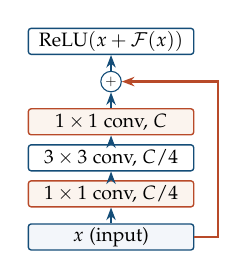
\begin{tikzpicture}[node distance=1.1mm,every node/.style={font=\tiny},
  bx/.style={box,minimum width=21mm,minimum height=3.3mm,inner sep=1pt}]
\node[bx,fill=soft] (in) {$x$ (input)};
\node[bx,draw=acc2,fill=soft2,above=2mm of in] (c1) {$1\times 1\text{ conv, } C/4$};
\node[bx,draw=acc,above=of c1] (c2) {$3\times 3\text{ conv, } C/4$};
\node[bx,draw=acc2,fill=soft2,above=of c2] (c3) {$1\times 1\text{ conv, } C$};
\node[circle,draw=acc,inner sep=0pt,minimum size=2.6mm,above=2mm of c3] (add) {$+$};
\node[bx,above=2mm of add] (out) {$\text{ReLU}(x + \mathcal{F}(x))$};
\draw[arr] (in)--(c1); \draw[arr] (c1)--(c2); \draw[arr] (c2)--(c3); \draw[arr] (c3)--(add); \draw[arr] (add)--(out);
\draw[arr,acc2,thick] (in.east) -- ++(3mm,0) |- (add.east);
\end{tikzpicture}
\end{minipage}\hfill
\begin{minipage}[t]{0.56\columnwidth}\vspace{1pt}\small
\textbf{The ResNet Bottleneck.} Stacks $1\times 1$ compress $\to 3\times 3$ spatial $\to 1\times 1$ expand. The skip connection carries the identity signal directly, preventing gradient vanishing:\\[2pt]
$\frac{\partial \mathcal{E}}{\partial x_l} = \frac{\partial \mathcal{E}}{\partial x_L} \left( \mathbf{I} + \frac{\partial}{\partial x_l} \sum_{i=l}^{L-1} \mathcal{F}_i(x_i) \right)$\\[2pt]
Even if gradients through $\mathcal{F}$ vanish ($\approx 0$), the identity $\mathbf{I}$ guarantees non-zero backpropagation back to layer $l$.
\end{minipage}

\begin{mem}[Convolution Arithmetic Formulas]
\begin{tabularx}{\linewidth}{@{}lL@{}}
$O = \lfloor \frac{I - K + 2P}{S} \rfloor + 1$ & Output spatial dimension (Input $I$, Kernel $K$, Pad $P$, Stride $S$)\\
$\text{FLOPs} = 2 C_{\text{in}} C_{\text{out}} K^2 H_o W_o$ & Exact multiply-adds ($2\times$ MACs) for standard Conv2D\\
$RF_l = RF_{l-1} + (K_l - 1) J_{l-1}$ & Receptive field of layer $l$; jump $J_l = J_{l-1} \cdot S_l$ ($J_0 = 1$)\\
$\frac{1}{C_{\text{out}}} + \frac{1}{K^2}$ & Computation ratio of Depthwise-Separable conv vs Standard Conv\\
\end{tabularx}
\end{mem}

\begin{qa}[Architecture Evolution \& Normalization Dynamics]
\Q{Derive the backpropagation gradient of Conv2D with respect to input $X$ and weights $W$.}{
Forward convolution: $Y_{c_{\text{out}}, i, j} = \sum_{c_{\text{in}}} \sum_{p=0}^{K-1} \sum_{q=0}^{K-1} W_{c_{\text{out}}, c_{\text{in}}, p, q} \cdot X_{c_{\text{in}}, i\cdot s + p, j\cdot s + q}$.
\begin{itemize}
\item \textbf{Gradient w.r.t Weights}: By chain rule:
$$\frac{\partial \mathcal{L}}{\partial W_{c_{\text{out}}, c_{\text{in}}, p, q}} = \sum_{i, j} \frac{\partial \mathcal{L}}{\partial Y_{c_{\text{out}}, i, j}} \cdot X_{c_{\text{in}}, i\cdot s + p, j\cdot s + q}$$
This is equivalent to a cross-correlation between the input activation $X$ and the upstream gradient $\frac{\partial \mathcal{L}}{\partial Y}$.
\item \textbf{Gradient w.r.t Input}:
$$\frac{\partial \mathcal{L}}{\partial X_{c_{\text{in}}, m, n}} = \sum_{c_{\text{out}}} \sum_{p, q} \frac{\partial \mathcal{L}}{\partial Y_{c_{\text{out}}, m - p, n - q}} \cdot W_{c_{\text{out}}, c_{\text{in}}, p, q}$$
This is equivalent to a full convolution of the upstream gradient with the \textbf{180-degree spatially flipped} kernel $W^{\text{rot180}}$ (padding with $K-1$).
\end{itemize}}
\Q{Why did VGG stack multiple $3\times 3$ convolutions instead of one $7\times 7$?}{
Three $3\times 3$ convolutions stacked with stride 1 have an effective receptive field of $1 + 3\times (3-1) = 7$, matching a single $7\times 7$ kernel.
\textbf{Parameter reduction}: $3 \cdot (3^2 C^2) = 27 C^2$ vs $1 \cdot (7^2 C^2) = 49 C^2$ ($45\%$ fewer weights).
\textbf{Expressivity}: Inserts three non-linear activation functions (ReLUs) rather than one, allowing more expressive discriminative functions.}
\Q{Why does BatchNorm fail on small batch sizes, and why is GroupNorm or SyncBN used?}{
BatchNorm normalizes across batch dimension $\mathcal{B}$: $\hat{x} = \frac{x - \mu_{\mathcal{B}}}{\sqrt{\sigma_{\mathcal{B}}^2 + \epsilon}}$.
In object detection and segmentation, high image resolutions restrict batch size per GPU to $B \in [2, 4]$.
At $B=2$, mini-batch mean $\mu_{\mathcal{B}}$ and variance $\sigma_{\mathcal{B}}^2$ exhibit extreme stochastic noise: batch statistics fluctuate wildly from step to step, corrupting training convergence and degrading test accuracy by $>5\%$.
\textbf{Solutions}:
\begin{enumerate}[leftmargin=*,itemsep=0.8pt]
\item \textbf{SyncBatchNorm}: Synchronizes mean and variance across all GPUs in distributed training via all-reduce, effectively restoring large virtual batch size ($B_{\text{effective}} = B_{\text{local}} \times N_{\text{GPUs}}$).
\item \textbf{GroupNorm (Wu \& He, 2018)}: Divides channels into $G=32$ groups and normalizes purely across channels and spatial pixels $(C/G, H, W)$. Independent of batch size $B$, ensuring stable training even at $B=1$.
\end{enumerate}}
\Q{What architectural innovations transform ResNet into ConvNeXt and ConvNeXt-V2?}{
Liu et al. modernize ResNet-50 by incorporating Vision Transformer design choices:
\begin{enumerate}[leftmargin=*,itemsep=0.8pt]
\item \textbf{Patchify Stem}: Replaces $7\times 7$ stride-2 conv $+$ max pooling with a non-overlapping $4\times 4$ stride-4 patchifying conv.
\item \textbf{Depthwise Inverted Bottleneck}: Uses $7\times 7$ depthwise convs placed \emph{before} $1\times 1$ pointwise convs, mimicking inverted residuals and Swin local window attention.
\item \textbf{Micro-Design}: Replaces BatchNorm with LayerNorm; replaces ReLU with GELU; reduces activation/normalization layers to one per block.
\item \textbf{ConvNeXt-V2 (Global Response Normalization)}: When trained with Masked Autoencoders (FCMAE), depthwise convs suffer from feature collapse where channels become redundant. ConvNeXt-V2 introduces \textbf{GRN} (Global Response Normalization) which scales channels by their L2 norm across spatial pixels, restoring feature diversity.
\end{enumerate}
Outperforms Swin Transformers across ImageNet, COCO, and ADE20K with purely convolutional operations.}
\end{qa}

\begin{trap}[Convolutional Gotchas]
\begin{itemize}
\item \textbf{Dilation Receptive Field}: Atrous/dilated conv with rate $r$ has effective kernel $K' = K + (K-1)(r-1)$. For $3\times 3$ with $r=2$, $K'=5$, growing receptive field without extra parameters.
\item \textbf{Gridding artifacts}: Stacking consecutive atrous convolutions with identical dilation rate $r$ creates "checkerboard" sampling holes. Fix: use hybrid dilated convolution (HDC) with coprime rates (e.g., $r=[1, 2, 5]$).
\end{itemize}
\end{trap}

\section{Modern ConvNets: MobileNet, ShuffleNet \& ConvNeXt}\label{sec:modern-conv}
\lab{Depthwise separable \textperiodcentered\ linear bottleneck \textperiodcentered\ channel shuffle \textperiodcentered\ compound scaling \textperiodcentered\ ConvNeXt \textperiodcentered\ GRN}

\diagpair{%
\adjustbox{max width=\linewidth}{%
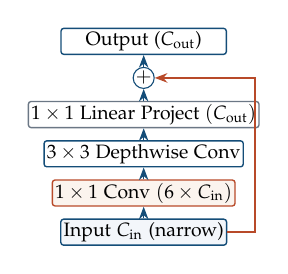
\begin{tikzpicture}[node distance=1.1mm,every node/.style={font=\scriptsize},
  bx/.style={box,minimum width=21mm,minimum height=3.3mm,inner sep=1pt}]
\node[bx,fill=soft] (in) {Input $C_{\text{in}}$ (narrow)};
\node[bx,draw=acc2,fill=soft2,above=1.5mm of in] (exp) {$1\times 1\text{ Conv } (6\times C_{\text{in}})$};
\node[bx,draw=acc,above=1.5mm of exp] (dw) {$3\times 3\text{ Depthwise Conv}$};
\node[bx,draw=mute,above=1.5mm of dw] (proj) {$1\times 1\text{ Linear Project } (C_{\text{out}})$};
\node[circle,draw=acc,inner sep=0pt,minimum size=2.6mm,above=1.5mm of proj] (add) {$+$};
\node[bx,above=1.5mm of add] (out) {Output ($C_{\text{out}}$)};
\draw[arr] (in)--(exp); \draw[arr] (exp)--(dw); \draw[arr] (dw)--(proj); \draw[arr] (proj)--(add); \draw[arr] (add)--(out);
\draw[arr,acc2,thick] (in.east) -- ++(3.5mm,0) |- (add.east);
\end{tikzpicture}%
}
}{%
\textbf{The Inverted Residual.} MobileNetV2 expands to high dimension ($t=6$) for depthwise filtering, then projects to low dimension with a linear bottleneck.\\[2pt]
{\color{acc2}$\blacktriangleright$} Standard ResNet: High $\to$ Low $\to$ High.\\
{\color{acc2}$\blacktriangleright$} Inverted: Low $\to$ High ($6\times$) $\to$ Low.\\
{\color{acc2}$\blacktriangleright$} Linear Bottleneck: Non-linear ReLU in low-dim collapses the manifold; projection must be purely linear.
}

\begin{mem}[Architectural Milestones in Modern Convolutions]
\begin{tabularx}{\columnwidth}{@{}p{19mm} p{23mm} X r@{}}
\toprule
\textbf{Model} & \textbf{Key Op} & \textbf{Core Innovation} & \textbf{Savings} \\
\midrule
\textbf{MobileNetV1} & Depthwise Sep. & Factorizes spatial ($K \times K$) and channel ($1 \times 1$) & $8-9\times$ \\
\textbf{MobileNetV2} & Inverted Resid. & Low $\to$ Exp $6\times \to$ DW $\to$ Linear project (no ReLU) & Low MAC \\
\textbf{ShuffleNetV2} & Channel Shuffle & Equal channel width minimizes memory access cost (MAC) & Fast GPU \\
\textbf{EfficientNet} & Compound Scale & Jointly scales depth $\alpha$, width $\beta$, and resolution $\gamma$ & Pareto SOTA \\
\textbf{ConvNeXt-V2} & GRN + 7x7 DW & Global Response Normalization solves MAE feature collapse & Beats Swin \\
\bottomrule
\end{tabularx}
\end{mem}

\begin{qa}[Depthwise Convolutions \& Bottleneck Dynamics]
\Q{Derive the exact FLOP reduction of Depthwise Separable Convolutions vs Standard Convolutions.}{
Let input feature map be $H \times W \times C_{\text{in}}$, output be $H \times W \times C_{\text{out}}$, and kernel size be $K \times K$:
\begin{itemize}
\item \textbf{Standard Convolution FLOPs}:
$$\text{FLOPs}_{\text{std}} = 2 \cdot H \cdot W \cdot C_{\text{in}} \cdot C_{\text{out}} \cdot K^2$$
\item \textbf{Depthwise Separable Convolution FLOPs}:
Composed of (1) Depthwise ($K \times K$ per channel) and (2) Pointwise ($1 \times 1$ conv):
$$\text{FLOPs}_{\text{sep}} = 2 \cdot H \cdot W \cdot C_{\text{in}} \cdot K^2 + 2 \cdot H \cdot W \cdot C_{\text{in}} \cdot C_{\text{out}} \cdot 1^2$$
\item \textbf{Theoretical Ratio}:
$$\frac{\text{FLOPs}_{\text{sep}}}{\text{FLOPs}_{\text{std}}} = \frac{C_{\text{in}} K^2 + C_{\text{in}} C_{\text{out}}}{C_{\text{in}} C_{\text{out}} K^2} = \frac{1}{C_{\text{out}}} + \frac{1}{K^2}$$
For standard $3 \times 3$ kernel ($K=3$) and large $C_{\text{out}} \gg 1$:
$$\frac{\text{FLOPs}_{\text{sep}}}{\text{FLOPs}_{\text{std}}} \approx \frac{1}{9} \approx 0.111 \quad \implies \quad \mathbf{\sim 8\text{ to }9\times \text{ FLOP reduction!}}$$
\end{itemize}}

\Q{Why does MobileNetV2 use Inverted Residuals with Linear Bottlenecks instead of classic ResNet bottlenecks?}{
\textbf{Classic ResNet Bottleneck}: High dimension $\to$ 1x1 reduce (channel compression) $\to$ 3x3 conv $\to$ 1x1 expand.
\textbf{MobileNetV2 Inverted Residual}: Low dimension (narrow) $\to$ 1x1 expand ($6\times$ channels) $\to$ 3x3 depthwise in high-dim $\to$ 1x1 project (narrow).
\begin{itemize}
\item \textbf{Why expand before depthwise?}: Depthwise convolutions cannot change channel count; performing depthwise filtering in low-dimensional space severely restricts representation capacity. Expanding channels by $t=6$ gives the depthwise filter an expressive manifold.
\item \textbf{Why Linear Bottleneck (no ReLU at output)?}: Applying a non-linear activation (ReLU) on low-dimensional manifolds destroys information: any negative values are zeroed out, collapsing dimensions. In high-dimensional representations, manifold features remain intact after ReLU; in low-dim bottlenecks, the projection must remain purely linear.
\end{itemize}}

\Q{Explain the ShuffleNet V2 design principles for practical inference latency on hardware.}{
Ma et al. showed that FLOPs do not correlate directly with wall-clock runtime; \textbf{Memory Access Cost (MAC)} dominates:
\begin{enumerate}
\item \textbf{Principle 1 (Equal channel width minimizes MAC)}: For $1 \times 1$ conv with FLOPs $B = H W C_1 C_2$, $\text{MAC} = H W (C_1 + C_2) + C_1 C_2 \ge 2\sqrt{H W B} + \frac{B}{H W}$. Equality holds when $C_1 = C_2$.
\item \textbf{Principle 2 (Excessive group convolution increases MAC)}: Large group count $g$ increases MAC for the same FLOP budget.
\item \textbf{Principle 3 (Network fragmentation reduces parallelism)}: Multi-branch paths (e.g., Inception, NAS architectures) fragment GPU kernel launches and reduce device utilization.
\item \textbf{Principle 4 (Element-wise operations have high MAC/FLOP ratio)}: Tensor addition, ReLU, and Squeeze-and-Excitation have negligible FLOPs but heavy memory round-trips.
\end{enumerate}}
\end{qa}

\begin{qa}[ConvNeXt Architecture \& Global Response Normalization]
\Q{How does ConvNeXt modernize standard ResNet-50 into a pure ConvNet competitive with Swin?}{
Liu et al. (2022) systematically modernized ResNet using ViT design principles:
\begin{itemize}
\item \textbf{Macro design}: ResNet stage ratio changed from $(3, 4, 6, 3)$ to $(3, 3, 9, 3)$ matching Swin.
\item \textbf{Patchify stem}: Replaced $7 \times 7$ conv (stride 2) + maxpool with a single $4 \times 4$ stride-4 convolution patchifying stem.
\item \textbf{Depthwise 7x7 conv}: Moved spatial conv before pointwise conv; enlarged kernel from $3 \times 3$ to $7 \times 7$ to match Swin's local window attention receptive field.
\item \textbf{Inverted bottleneck}: Expanded channel width $4\times$ inside each block (like ViT MLP expansion ratio 4).
\item \textbf{Activation \& Normalization}: Replaced ReLU with GELU; reduced activations to 1 per block; replaced BatchNorm with LayerNorm.
\end{itemize}}

\Q{What is Global Response Normalization (GRN) in ConvNeXt-V2, and why does it prevent feature collapse?}{
When training ConvNeXt with Masked Autoencoders (FCMAE), masked feature channels exhibit feature collapse (redundant/dead channels with near-identical activation maps).
\textbf{GRN mechanism} computes spatial $L_2$ norm per channel, normalizes across channels, and recalibrates:
\begin{enumerate}
\item \textbf{Global feature aggregation}: $g_c = \| X_c \|_2 = \sqrt{\sum_{i,j} X_c(i,j)^2}$.
\item \textbf{Channel response normalization}: $n_c = \frac{g_c}{\frac{1}{C}\sum_{c'} g_{c'}}$.
\item \textbf{Feature calibration}: $X_c' = \gamma \cdot (X_c \odot n_c) + \beta + X_c$, initialized with $\gamma=0, \beta=0$.
\end{enumerate}
GRN creates channel competition: active channels suppress redundant passive channels, preventing representation collapse in self-supervised pretraining.}
\end{qa}

\begin{trap}[Modern ConvNet Hardware Traps]
\begin{itemize}
\item \textbf{Depthwise Conv Slowdown on GPUs}: Depthwise convolutions have extremely low compute-to-memory ratio (arithmetic intensity). On GPUs without specialized Tensor Core depthwise acceleration, standard $3 \times 3$ dense convs often execute faster than depthwise convs despite higher theoretical FLOPs!
\item \textbf{Fused 1x1 Convolutions}: Inverted bottleneck blocks should use kernel fusion ($1 \times 1 \to 3 \times 3 \to 1 \times 1$) in TensorRT/TorchScript to avoid multiple intermediate DRAM round-trips.
\end{itemize}
\end{trap}

\section{Vision Transformers (ViT), Scaling \& Tokenization}\label{sec:vit}
\lab{patch embedding \textperiodcentered\ inductive bias \textperiodcentered\ DeiT distillation \textperiodcentered\ 2D PosEnc \textperiodcentered\ NaViT patch packing}

\diagpair{%
\adjustbox{max width=\linewidth}{%
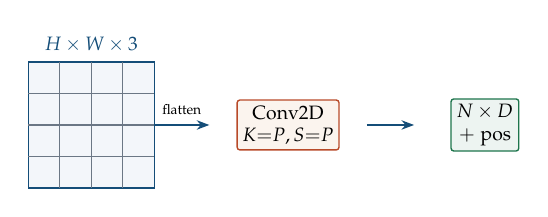
\begin{tikzpicture}[x=1mm,y=1mm,every node/.style={font=\scriptsize}]
\draw[draw=acc,fill=soft] (0,0) rectangle (16,16);
\foreach \x in {4,8,12} \draw[mute] (\x,0) -- (\x,16);
\foreach \y in {4,8,12} \draw[mute] (0,\y) -- (16,\y);
\node[acc,above] at (8,16) {$H \times W \times 3$};
\draw[arr] (16,8) -- (23,8) node[midway,above,font=\tiny] {flatten};
\node[box,draw=acc2,fill=soft2] at (33,8) {Conv2D\\$K{=}P, S{=}P$};
\draw[arr] (43,8) -- (49,8);
\node[box,draw=acc3,fill=acc3!8] at (58,8) {$N \times D$\\$+$ pos};
\end{tikzpicture}%
}
}{%
\textbf{Image to Sequence.} An image $x \in \mathbb{R}^{H\times W\times C}$ is split into $N = \frac{HW}{P^2}$ patches of size $P\times P$. Linear projection projects each patch to dimension $D$ (equivalent to Conv2D with kernel $P$, stride $P$, $D$ filters):\\[2pt]
$\mathbf{z}_0 = [\mathbf{x}_{\text{cls}};\, \mathbf{x}_p^1 \mathbf{E}; \dots;\, \mathbf{x}_p^N \mathbf{E}] + \mathbf{E}_{\text{pos}}$\\[2pt]
where $\mathbf{E} \in \mathbb{R}^{(P^2 C)\times D}$ and $\mathbf{E}_{\text{pos}} \in \mathbb{R}^{(N+1)\times D}$.
}

\begin{mem}[Standard ViT Model Configurations \& Scaling]
\begin{tabularx}{\linewidth}{@{}lccccL@{}}
\toprule
\textbf{Model} & \textbf{Layers} & \textbf{Hidden $D$} & \textbf{Heads} & \textbf{MLP Dim} & \textbf{Params (GMACs, $224^2$)}\\
\midrule
ViT-B/16 & 12 & 768 & 12 & 3072 & 86M (17.6)\\
ViT-L/16 & 24 & 1024 & 16 & 4096 & 307M (61.6)\\
ViT-H/14 & 32 & 1280 & 16 & 5120 & 632M (167.4)\\
ViT-g/14 & 40 & 1408 & 16 & 6144 & 1.0B (284.1)\\
ViT-22B  & 48 & 6144 & 48 & 24576& 22B ($\sim$4.4k)\\
\bottomrule
\end{tabularx}
\end{mem}

\begin{qa}[Inductive Bias, Distillation \& Tokenization]
\Q{Why do CNNs outperform ViTs on small datasets, but lose at scale?}{
\textbf{Inductive Biases}: CNNs hardcode \emph{translation equivariance} ($f(g(x)) = g(f(x))$) and \emph{locality} (pixels close together interact first). This provides a massive data-efficiency inductive prior.
\textbf{ViT}: Has almost zero 2D prior; self-attention is permutation-equivariant, and spatial structure must be learned entirely through $\mathbf{E}_{\text{pos}}$ and attention weights.
\textbf{Empirical inflection point}: Under $\approx 10\text{M}$ images (ImageNet-1K), ResNet outperforms standard ViT. Above $100\text{M}$ images (ImageNet-21K, JFT-300M), ViT's higher capacity scales monotonically without saturating.}
\Q{How does DeiT achieve high accuracy on pure ImageNet-1K?}{
Touvron et al. introduce \textbf{hard distillation}:
\begin{enumerate}
\item \textbf{Distillation Token}: Appends a learnable \texttt{[DIST]} token alongside \texttt{[CLS]}. The distillation token interacts with patches via self-attention and is supervised by a CNN teacher's hard label:
$$\mathcal{L} = \frac{1}{2} \mathcal{L}_{\text{CE}}(y, \sigma(z_{\text{cls}})) + \frac{1}{2} \mathcal{L}_{\text{CE}}(y_{\text{teacher}}, \sigma(z_{\text{dist}}))$$
\item \textbf{Heavy Regularization}: Mixup ($\alpha=0.8$), CutMix ($\alpha=1.0$), RandAugment, Stochastic Depth, and repeated augmentations prevent overfitting the unconstrained attention maps.
\end{enumerate}
Reaches $85.2\%$ top-1 on ImageNet-1K without external pretraining.}
\Q{How do Mean Attention Distance and layer depth behave across a trained ViT?}{
Define Mean Attention Distance for head $h$ at layer $l$:
$$\bar{D}_{l, h} = \sum_{j=1}^N A_{i, j}^{(l, h)} \cdot \|\mathbf{p}_i - \mathbf{p}_j\|_2$$
where $\mathbf{p}_i$ is the 2D spatial coordinate of patch $i$.
\textbf{In shallow layers ($l=1\dots 4$)}: Different heads specialize. Several heads have tiny attention distance ($\bar{D} \approx 2-4$ patches), acting exactly like localized $3\times 3$ convolutional filters; other heads attend globally.
\textbf{In deep layers ($l=8\dots 12$)}: Attention distance is universally large across almost all heads ($\bar{D} \approx 10-14$ patches), performing global scene integration and semantic classification across the entire image.}
\Q{How does NaViT (Patch n' Pack) resolve aspect ratio distortion and padding waste?}{
Standard ViTs resize images to fixed square shapes ($224\times 224$), causing non-square camera pictures (e.g., $16:9$) to stretch and distort geometric aspect ratios. Alternatively, padding with black bars wastes up to $50\%$ of sequence FLOPs on empty border tokens.
\textbf{NaViT (Dehghani et al., 2023)}:
\begin{enumerate}
\item \textbf{Patch n' Pack}: Packs patches from multiple distinct images with arbitrary resolutions and aspect ratios into a single sequence of length $L$ (e.g., $L=4096$).
\item \textbf{Self-Attention Masking}: Uses an attention mask that forbids tokens from different images within the packed sequence from attending to each other.
\item \textbf{2D Continuous Positional Encodings}: Queries and keys receive 2D fractional coordinates $(x/W, y/H) \in [0, 1]^2$.
\end{enumerate}
Eliminates all padding waste, preserves native image aspect ratios, and increases training throughput by $4-5\times$.}
\end{qa}

\begin{trap}[ViT Attention Traps]
\begin{itemize}
\item \textbf{Quadratic token cost}: Doubling image resolution quadruples the token sequence length $N$, which increases self-attention computation and activation memory by $16\times$ ($\mathcal{O}(N^2)$).
\item \textbf{Bicubic vs Nearest for PosEnc}: Using nearest-neighbor interpolation causes high-frequency spatial artifacts and loss spikes during high-res fine-tuning. Bicubic maintains smooth positional phases.
\end{itemize}
\end{trap}

\section{Hierarchical Vision Transformers: Swin \& Hybrids}\label{sec:swin}
\lab{Swin Transformer \textperiodcentered\ shifted windows \textperiodcentered\ patch merging \textperiodcentered\ cyclic masking \textperiodcentered\ CoAtNet \textperiodcentered\ FastViT}

\noindent\begin{minipage}[t]{0.42\columnwidth}\vspace{0pt}\centering
\resizebox{\linewidth}{!}{%
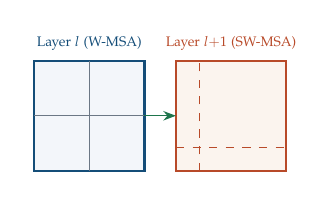
\begin{tikzpicture}[x=1mm,y=1mm,every node/.style={font=\tiny}]
% Layer l: regular window
\draw[draw=acc,fill=soft,thick] (0,10) rectangle (14,24);
\draw[mute] (7,10) -- (7,24); \draw[mute] (0,17) -- (14,17);
\node[acc,above] at (7,24) {Layer $l$ (W-MSA)};
% Layer l+1: shifted window
\draw[draw=acc2,fill=soft2,thick] (18,10) rectangle (32,24);
\draw[acc2,dashed] (21,10) -- (21,24); \draw[acc2,dashed] (18,13) -- (32,13);
\node[acc2,above] at (25,24) {Layer $l{+}1$ (SW-MSA)};
\draw[arr,acc3] (14,17) -- (18,17);
\end{tikzpicture}%
}
\end{minipage}\hfill
\begin{minipage}[t]{0.56\columnwidth}\vspace{1pt}\small
\textbf{Linear Complexity Vision.} Standard global ViT self-attention scales quadratically: $\mathcal{O}(H^2 W^2)$. Swin restricts self-attention to local $M\times M$ windows ($M=7$):
$$\Omega(\text{W-MSA}) = 4hwC^2 + 2M^2 hwC$$
Linear in image area $hw$. To exchange cross-window information without global attention, consecutive blocks alternate between standard and \textbf{shifted} window partitions.
\end{minipage}

\begin{mem}[Hierarchical Feature Pyramid (Swin vs ViT)]
\begin{itemize}
\item \textbf{Patch Merging}: Concatenates features of each $2\times 2$ neighborhood ($4C$-dim), applies a linear layer to produce $2C$-dim. Halves spatial resolution while doubling channels (produces $\frac{H}{4}, \frac{H}{8}, \frac{H}{16}, \frac{H}{32}$ pyramids compatible with FPN).
\item \textbf{Cyclic Shift \& Masking}: Naive shifted window partitioning yields up to $2\times 2$ extra partial windows at boundaries. Swin performs a cyclic shift to assemble partial windows into regular $M\times M$ windows, computes attention with a masking matrix $\mathbf{M}$ that blocks non-adjacent tokens, then reverse shifts.
\item \textbf{Relative Position Bias}: Adds bias matrix $\mathbf{B} \in \mathbb{R}^{M^2 \times M^2}$ from learned table $\hat{B} \in \mathbb{R}^{(2M-1)\times (2M-1)}$ based on coordinate offsets $(\Delta x, \Delta y) \in [-M+1, M-1]$.
\end{itemize}
\end{mem}

\begin{qa}[Dense Prediction, Window Attention \& Hybrids]
\Q{Why can't standard ViT directly replace ResNet in Faster R-CNN or U-Net?}{
\textbf{1. Single-scale representation}: ViT maintains constant token resolution ($\frac{H}{16} \times \frac{W}{16}$) throughout all depth. FPN and U-Net require multi-scale pyramids ($C_2, C_3, C_4, C_5$) to detect objects across small, medium, and large scales.
\textbf{2. High-resolution memory explosion}: Object detection and segmentation require large inputs ($1024\times 1024$ or $1333\times 800$). At $P=16$, $1024^2 \implies 4096$ tokens, whose $N^2$ attention map consumes $4096^2 \times 2\text{ bytes} = 33.5\text{ MB}$ per head, overflowing GPU VRAM during training.}
\Q{How does the Swin attention mask prevent cyclic leakage?}{
A cyclic shift wraps border tokens from the top-left to the bottom-right of the feature map, packing multiple disconnected image patches into the same $M\times M$ window.
The attention mask $\mathbf{M}$ assigns $-\infty$ to logit entries $(i, j)$ if tokens $i$ and $j$ originated from different sub-windows before the shift:
$$\text{Attention} = \text{Softmax}\left(\frac{QK^\top}{\sqrt{d}} + B + M\right) V$$
$\text{Softmax}(\cdot)$ zeros out cross-patch attention weights, computing identical values to separate window evaluations in a single dense batched kernel without kernel launch overhead.}
\Q{How does Pyramid Vision Transformer (PVT) achieve multi-scale representations without windows?}{
Wang et al. maintain global self-attention across the full image while reducing complexity via \textbf{Spatial-Reduction Attention (SRA)}:
Instead of attending to all $N$ tokens, keys and values are spatially downsampled by reduction ratio $R_i$ using a strided convolution before projection:
$$\hat{K} = \operatorname{Linear}(\operatorname{Conv2D}(x, R_i)), \quad \hat{V} = \operatorname{Linear}(\operatorname{Conv2D}(x, R_i))$$
Reduces keys/values from $N$ to $N / R_i^2$.
Complexity drops from $\mathcal{O}(N^2)$ to $\mathcal{O}(N^2 / R_i^2)$, allowing global receptive fields in shallow stages with manageable memory.}
\Q{What is CoAtNet's recipe for combining Convolutions and Attention?}{
Dai et al. organize blocks into 5 stages:
\begin{itemize}
\item \textbf{Stage 0--1 (Conv)}: Standard $3\times 3$ conv and depthwise convs (captures low-level local edges and textures cheaply where spatial resolution is huge).
\item \textbf{Stage 2--3 (Attention + Conv)}: Relative self-attention fused with depthwise convolution:
$$y = \text{Softmax}\left(\frac{QK^\top}{\sqrt{d}} + W_{\text{conv}} + B\right) V$$
\end{itemize}
Balances inductive bias in shallow layers with global semantic reasoning in deep layers, achieving $86.0\%$ top-1 on ImageNet-1K with fast training.}
\end{qa}

\begin{trap}[Swin Implementation Gotchas]
\begin{itemize}
\item \textbf{Dynamic image sizing in Swin}: If $H$ or $W$ is not a multiple of $M \cdot 2^{\text{stages}-1} = 7 \cdot 8 = 56$, inputs must be padded. Omitting pad/unpad logic creates silent spatial coordinate warping.
\item \textbf{Batch dimension in Window Attention}: Folding spatial windows into batch $(B \cdot N_w, M^2, C)$ requires memory contiguity (\lstinline|.contiguous().view(...)|); failure to ensure contiguity triggers silent stride errors on CUDA.
\end{itemize}
\end{trap}

\section{Object Detection: Two-Stage Detectors, FPN \& mAP}\label{sec:det}
\lab{Faster R-CNN \textperiodcentered\ RPN anchors \textperiodcentered\ RoIAlign \textperiodcentered\ FPN \textperiodcentered\ CIoU Loss \textperiodcentered\ COCO mAP}

\diagpair{%
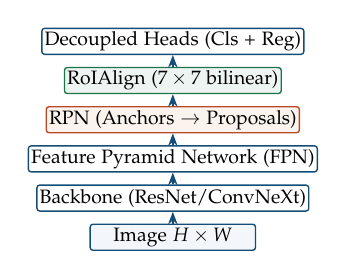
\begin{tikzpicture}[node distance=1.1mm,every node/.style={font=\scriptsize},
  bx/.style={box,minimum width=21mm,minimum height=3.3mm,inner sep=1pt}]
\node[bx,fill=soft] (img) {Image $H\times W$};
\node[bx,above=1.5mm of img] (bb) {Backbone (ResNet/ConvNeXt)};
\node[bx,above=1.5mm of bb] (fpn) {Feature Pyramid Network (FPN)};
\node[bx,draw=acc2,fill=soft2,above=1.5mm of fpn] (rpn) {RPN (Anchors $\to$ Proposals)};
\node[bx,draw=acc3,fill=acc3!8,above=1.5mm of rpn] (align) {RoIAlign ($7\times 7$ bilinear)};
\node[bx,above=1.5mm of align] (fc) {Decoupled Heads (Cls + Reg)};
\draw[arr] (img)--(bb); \draw[arr] (bb)--(fpn); \draw[arr] (fpn)--(rpn); \draw[arr] (rpn)--(align); \draw[arr] (align)--(fc);
\end{tikzpicture}
}{%
\textbf{The Object Detection Paradigm.} Predicts class label $c \in \{1,\dots,K\}$ and coordinates $\mathbf{b} = [x_1, y_1, x_2, y_2]$ for all instances.\\[2pt]
{\color{acc2}$\blacktriangleright$} \textbf{FPN}: Combines semantic richness of deep layers with high spatial resolution of shallow layers via top-down pathways and lateral $1\times 1$ conv additions.\\
{\color{acc2}$\blacktriangleright$} \textbf{Decoupled Head}: Separate conv branches for classification (invariant to translation) and regression (sensitive to translation).
}

\begin{mem}[RoI Operations: Pool vs Align]
\begin{tabularx}{\linewidth}{@{}lLL@{}}
\toprule
\textbf{Operation} & \textbf{Coordinate Handling} & \textbf{Consequence}\\
\midrule
\textbf{RoIPool} (Fast R-CNN) & Rounds continuous RoI coordinates to feature stride ($x/16$), then rounds sub-cell bins. & Quantization error introduces severe sub-pixel spatial shifts; destroys mask AP.\\
\textbf{RoIAlign} (Mask R-CNN) & No quantization. Uses exact floating coordinates; samples 4 points per bin via \textbf{bilinear interpolation}. & Eliminates coordinate misalignment; gains $+3.0$ box AP and enables pixel-precise instance masks.\\
\bottomrule
\end{tabularx}
\end{mem}

\begin{qa}[Detection Mechanics, Losses \& YOLO Evolution]
\Q{State the Complete IoU (CIoU) loss formulation and explain why it outperforms GIoU.}{
Standard GIoU penalizes empty area inside the smallest enclosing convex hull $C$: $\text{GIoU} = \text{IoU} - \frac{|C \setminus (A \cup B)|}{|C|}$. When one box is completely inside another, GIoU degenerates to standard IoU.
\textbf{CIoU (Zheng et al., 2020)} incorporates 3 geometric factors simultaneously:
$$\mathcal{L}_{\text{CIoU}} = 1 - \text{IoU} + \frac{\rho^2(\mathbf{b}, \mathbf{b}^{\text{gt}})}{c^2} + \alpha v$$
\begin{itemize}
\item $\frac{\rho^2(\mathbf{b}, \mathbf{b}^{\text{gt}})}{c^2}$: Normalized Euclidean distance between box center points, where $c$ is diagonal length of the smallest enclosing box.
\item $v = \frac{4}{\pi^2} \left( \arctan \frac{w^{\text{gt}}}{h^{\text{gt}}} - \arctan \frac{w}{h} \right)^2$: Measures aspect ratio consistency.
\item $\alpha = \frac{v}{(1 - \text{IoU}) + v}$: Non-overlapping balance parameter giving high priority to aspect ratio when IoU is high.
\end{itemize}
Accelerates convergence and improves localization accuracy across tight multi-scale boxes.}
\Q{How does Faster R-CNN's Region Proposal Network generate and train proposals?}{
A $3\times 3$ conv slides over each FPN level; every location holds $k$ anchors (aspect ratios $\{1{:}2, 1{:}1, 2{:}1\}$, one scale per level, areas $32^2 \to 512^2$). Two sibling $1\times 1$ heads output $k$ objectness logits and $4k$ box deltas.\\
\textbf{Box encoding} relative to anchor $(x_a, y_a, w_a, h_a)$:
$$t_x = \tfrac{x - x_a}{w_a},\; t_y = \tfrac{y - y_a}{h_a},\; t_w = \log\tfrac{w}{w_a},\; t_h = \log\tfrac{h}{h_a}$$
\textbf{Labels}: positive if IoU $> 0.7$ with a GT (or the best anchor for that GT), negative if $< 0.3$, otherwise ignored. Sample 256 anchors per image at up to $1{:}1$ pos:neg; loss is BCE $+$ Smooth-L1 on positives.\\
\textbf{Inference}: decode, keep the top $\sim$2000 per level, NMS at 0.7, keep 1000 proposals $\to$ RoIAlign $\to$ second stage (512 RoIs/image in training, 25\% positives at IoU $\ge 0.5$).}
\Q{How does FPN build its pyramid, and which level does an RoI read from?}{
The backbone gives $C_2 \dots C_5$ (strides 4 to 32). Top-down: $P_5 = \text{conv}_{1\times 1}(C_5)$, then $P_l = \text{Up}_{2\times}(P_{l+1}) + \text{conv}_{1\times 1}(C_l)$, followed by a $3\times 3$ conv per level to reduce upsampling aliasing. All levels have 256 channels, so every level carries strong semantics at its native resolution.\\
\textbf{RoI-to-level rule}: $k = \big\lfloor k_0 + \log_2(\sqrt{wh}/224) \big\rfloor$, $k_0 = 4$, clamped to $[2, 5]$. A $224^2$ RoI reads $P_4$, a $112^2$ RoI reads $P_3$: small objects use fine maps, large objects use coarse semantic maps.}
\Q{How is COCO mAP actually computed?}{
Per class and IoU threshold: sort every detection in the dataset by score; match each greedily to the highest-IoU unmatched GT (crowd regions ignored). A match above the threshold is a TP, anything else an FP. Sweeping the score gives the PR curve; make precision monotone, $p(r) = \max_{r' \ge r} p(r')$, and average it at 101 recall points $\{0, 0.01, \dots, 1\}$: that is AP.\\
\textbf{mAP} $=$ mean over 80 classes and 10 thresholds $0.50{:}0.05{:}0.95$. $\text{AP}_S / \text{AP}_M / \text{AP}_L$ split by area $< 32^2$, $32^2$--$96^2$, $> 96^2$. At most 100 detections per image are scored, which is why evaluation uses a 0.001 score threshold.}
\end{qa}

\begin{trap}[Detection Metric Traps]
\begin{itemize}
\item \textbf{COCO mAP vs VOC AP}: VOC 2007 measures AP at a single threshold $\text{IoU} = 0.50$ ($\text{mAP}_{50}$). COCO reports average AP over 10 thresholds: $[0.50:0.05:0.95]$ ($\text{mAP}_{50:95}$). A model can achieve $85\%$ on $\text{mAP}_{50}$ but drop to $55\%$ on $\text{mAP}_{50:95}$ due to loose box boundary localization.
\item \textbf{Bounding box parametrization}: $(x, y, w, h)$ center vs $(x_1, y_1, x_2, y_2)$ corner format. Mixing them up produces negative width/height in regression branches.
\end{itemize}
\end{trap}

\section{Single-Stage Detectors: RetinaNet \& The YOLO Lineage}\label{sec:yolo}
\lab{SSD \textperiodcentered\ Focal Loss \textperiodcentered\ YOLOv1--v11 evolution \textperiodcentered\ Anchor-free \textperiodcentered\ TAL assigner \textperiodcentered\ DFL \textperiodcentered\ NMS-free YOLOv10}

\noindent\begin{minipage}[t]{0.42\columnwidth}\vspace{0pt}\centering
\resizebox{\linewidth}{!}{%
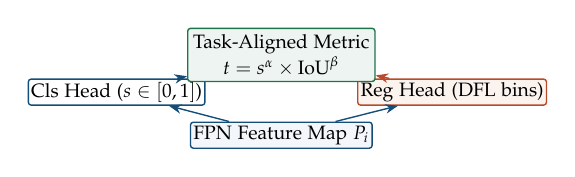
\begin{tikzpicture}[node distance=1.1mm,every node/.style={font=\tiny},
  bx/.style={box,minimum width=21mm,minimum height=3.3mm,inner sep=1pt}]
\node[bx,fill=soft] (feat) {FPN Feature Map $P_i$};
\node[bx,draw=acc,above left=2mm and -2mm of feat] (cls) {Cls Head ($s \in [0, 1]$)};
\node[bx,draw=acc2,fill=soft2,above right=2mm and -2mm of feat] (reg) {Reg Head (DFL bins)};
\node[box,draw=acc3,fill=acc3!8,above=5mm of feat] (tal) {Task-Aligned Metric\\$t = s^\alpha \times \text{IoU}^\beta$};
\draw[arr] (feat) -- (cls); \draw[arr] (feat) -- (reg);
\draw[arr,acc] (cls) -- (tal); \draw[arr,acc2] (reg) -- (tal);
\end{tikzpicture}%
}
\end{minipage}\hfill
\begin{minipage}[t]{0.56\columnwidth}\vspace{1pt}\small
\textbf{The Decoupled Anchor-Free Head.} Modern YOLO (v8--v11) splits classification from localization.\\[2pt]
{\color{acc2}$\blacktriangleright$} \textbf{TAL Alignment}: Top-$k$ candidates ranked by joint metric $t = s^\alpha \times \text{IoU}^\beta$ to eliminate misalignment.\\
{\color{acc2}$\blacktriangleright$} \textbf{DFL Head}: Predicts continuous box boundaries as probability distributions across 16 discrete distance bins.
\end{minipage}

\begin{mem}[The Full YOLO Evolution Timeline (v1 to v11)]
\begin{tabularx}{\columnwidth}{@{}p{14mm} p{17mm} X r@{}}
\toprule
\textbf{Model} & \textbf{Head Type} & \textbf{Core Architectural Innovations} & \textbf{NMS / Post} \\
\midrule
\textbf{YOLOv1} & Coupled Grid & First real-time detector ($7\times 7$ grid, FC regression) & Grid ownership \\
\textbf{YOLOv3} & Anchor-based & Darknet-53 + FPN multi-scale heads (P3, P4, P5) & K-means IoU \\
\textbf{YOLOv4/5} & Anchor-based & CSPDarknet backbone + PANet neck + Mosaic augment & IoU threshold \\
\textbf{YOLOv7} & Anchor-based & E-ELAN + RepConv structural re-parameterization & Lead assigner \\
\textbf{YOLOv8} & Anchor-free & Decoupled head + C2f block + Distribution Focal Loss & TAL Assigner \\
\textbf{YOLOv9} & Anchor-free & Programmable Gradient Information (PGI) + GELAN & Aux matching \\
\textbf{YOLOv10} & Dual-head & Dual assignments: 1-to-many train, 1-to-1 infer & \hl{Zero NMS ms} \\
\textbf{YOLOv11} & Anchor-free & C3k2 blocks + optimized depth/width scaling for NPUs & TAL + DFL \\
\bottomrule
\end{tabularx}
\end{mem}

\begin{qa}[Focal Loss \& Label Assignment Strategies]
\Q{Derive Focal Loss and mathematically demonstrate why it prevents easy negative gradients from swamping training.}{
Standard binary cross entropy (CE) loss is $\text{CE}(p_t) = -\log(p_t)$, where $p_t = p$ if $y=1$ and $p_t = 1-p$ if $y=0$.
In dense single-stage detection, over $100,000$ candidate anchors exist, with $\sim 99.9\%$ being easy background negatives ($p_t \approx 0.99$).
Although $\text{CE}(0.99) \approx 0.01$ is small, summing over $10^5$ candidates yields a gradient magnitude that completely overwhelms the few rare foreground positive targets ($p_t \approx 0.1$).\\[2pt]
\textbf{Focal Loss Formulation}:
$$\text{FL}(p_t) = -\alpha_t (1 - p_t)^\gamma \log(p_t) \quad (\text{typically } \gamma = 2.0, \alpha = 0.25)$$
\textbf{Gradient Dynamics}:
The gradient with respect to logit $z$ ($p_t = \sigma(z)$) is:
$$\frac{\partial \text{FL}}{\partial z} = \alpha_t (1 - p_t)^\gamma \left( p_t - y \right) + \gamma \alpha_t (1 - p_t)^{\gamma-1} p_t (1 - p_t) \log(p_t)$$
For an easy background sample ($p_t = 0.99$):
The modulating factor is $(1 - 0.99)^2 = (0.01)^2 = 0.0001$ --- a \hl{$10,000\times$ gradient suppression}!
For a hard positive or misclassified sample ($p_t = 0.2$):
$(1 - 0.2)^2 = 0.64$ --- virtually unaffected. The loss automatically focuses learning on hard informative candidates.}

\Q{Compare Anchor-based vs Anchor-free detection: why did modern YOLO architectures abandon anchors?}{
\begin{itemize}
\item \textbf{Flaws of Anchor-based}: Requires manual heuristic tuning of anchor aspect ratios and scales (often dataset-specific k-means); dense spatial tiling creates hundreds of thousands of anchors, $99\%$ of which are wasted; fixed IoU thresholds (e.g., $0.5$) for positive matching fail on extreme-aspect objects.
\item \textbf{Anchor-free Paradigm}: Predicts distance offsets from a grid point $(x, y)$ directly to the 4 box boundaries $(l, t, r, b)$, eliminating hyperparameter tuning and dramatically simplifying feature heads.
\end{itemize}}

\Q{How does Task-Aligned Assigner (TAL) in YOLOv8/v11 prevent the misalignment between classification and localization?}{
Traditional assigners treat classification and regression independently: an anchor might have high classification score but poor IoU, or high IoU but low confidence. When Non-Maximum Suppression (NMS) ranks predictions solely by classification score, it retains boxes with poor spatial overlap and suppresses well-localized boxes.\\[2pt]
\textbf{TAL Metric}: Computes a joint alignment metric $t$ for each candidate anchor $i$ and ground truth $j$:
$$t = s^\alpha \times \text{IoU}^\beta \quad (\text{default: } \alpha = 0.5, \beta = 6.0)$$
where $s$ is the predicted class probability and $\text{IoU}$ is the predicted box overlap with ground truth.
Top-$k$ candidates with the highest alignment metric $t$ are assigned as positive samples.
Furthermore, the classification target is dynamically scaled to $t$ rather than a binary $\{0, 1\}$, forcing high classification scores to strictly coincide with high IoU accuracy.}
\end{qa}

\begin{qa}[DFL \& NMS-Free End-to-End YOLOv10]
\Q{What is Distribution Focal Loss (DFL) and why does it improve boundary precision?}{
Standard detectors predict a single deterministic scalar for bounding box offsets: $y \in \mathbb{R}$. However, in complex real-world scenes with blurry or occluded edges, the true boundary is inherently uncertain.\\[2pt]
\textbf{DFL Formulation}: Predicts a discrete probability distribution over $n$ intervals $\{y_0, y_1, \dots, y_n\}$ (e.g., $16$ bins):
$$\hat{y} = \sum_{i=0}^n \operatorname{softmax}(S_i) \cdot y_i$$
DFL minimizes the cross-entropy between the predicted distribution and the two discrete bins $[y_i, y_{i+1}]$ that flank the continuous ground truth $y$:
$$\mathcal{L}_{\text{DFL}}(S_i, S_{i+1}) = - \left( (y_{i+1} - y) \log(S_i) + (y - y_i) \log(S_{i+1}) \right)$$
This enables the network to express spatial uncertainty (sharp peak = clear edge; wide flat distribution = blurry/occluded boundary).}

\Q{How does YOLOv10 eliminate NMS post-processing while maintaining high training accuracy?}{
\textbf{The Dilemma}: One-to-one matching (Hungarian assignment) enables NMS-free inference (like DETR) but suffers from slow training convergence due to sparse supervision. One-to-many matching provides rich supervisory gradients but produces duplicate boxes requiring NMS.\\[2pt]
\textbf{YOLOv10 Dual-Label Assignment}:
\begin{itemize}
\item \textbf{Training}: Evaluates two parallel heads sharing the same backbone/neck: (1) a one-to-many head (optimizing gradient flow and representation learning) and (2) a one-to-one head (optimizing direct, unique prediction).
\item \textbf{Harmonized Matching}: Adjusts metric alignment so both heads learn mutually consistent representations.
\item \textbf{Inference}: Discards the one-to-many head completely! Runs only the one-to-one head, yielding zero-duplicate predictions with \hl{0 ms post-processing latency}.
\end{itemize}}
\end{qa}

\begin{trap}[YOLO Production Traps]
\begin{itemize}
\item \textbf{Input Resolution Aspect Ratio Distortion}: Directly resizing images of arbitrary aspect ratios (e.g. $1920 \times 1080$) to square $640 \times 640$ distorts spatial aspect ratios, degrading small object recall. Always use letterboxing with gray padding, and ensure padding is aligned to a stride multiple of 32.
\item \textbf{NMS Confidence Threshold Tuning}: Setting NMS confidence threshold too high (e.g. $>0.5$) severely kills mAP on small objects. Standard COCO evaluation uses confidence threshold $0.001$ with NMS IoU threshold $0.65$.
\end{itemize}
\end{trap}

\section{Query-Based Detection: DETR, Deformable DETR \& RT-DETR}\label{sec:detr}
\lab{DETR \textperiodcentered\ Hungarian matching \textperiodcentered\ bipartite set loss \textperiodcentered\ Deformable Attention \textperiodcentered\ DINO-DETR \textperiodcentered\ RT-DETR}

\diagpair{%
\adjustbox{max width=\linewidth}{%
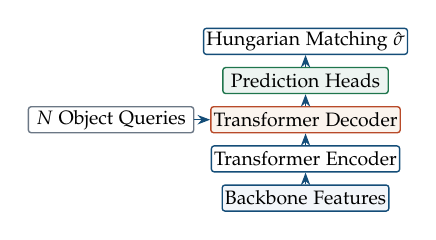
\begin{tikzpicture}[node distance=1.1mm,every node/.style={font=\scriptsize},
  bx/.style={box,minimum width=21mm,minimum height=3.3mm,inner sep=1pt}]
\node[bx,fill=soft] (bb) {Backbone Features};
\node[bx,draw=acc,above=1.5mm of bb] (enc) {Transformer Encoder};
\node[bx,draw=acc2,fill=soft2,above=1.5mm of enc] (dec) {Transformer Decoder};
\node[bx,draw=mute,left=2mm of dec] (q) {$N$ Object Queries};
\node[bx,draw=acc3,fill=acc3!8,above=1.5mm of dec] (ffn) {Prediction Heads};
\node[bx,above=1.5mm of ffn] (hung) {Hungarian Matching $\hat{\sigma}$};
\draw[arr] (bb)--(enc); \draw[arr] (enc)--(dec); \draw[arr] (q)--(dec); \draw[arr] (dec)--(ffn); \draw[arr] (ffn)--(hung);
\end{tikzpicture}%
}
}{%
\textbf{Direct Set Prediction.} Bypasses hand-designed anchor boxes and greedy NMS entirely. Formulates detection as predicting an unordered set of $N$ bounding boxes (e.g., $N=300$).\\[2pt]
{\color{acc2}$\blacktriangleright$} One-to-one matching enforces that each ground-truth object is assigned to exactly \textbf{one} query.\\
{\color{acc2}$\blacktriangleright$} No duplicate predictions $\implies$ zero NMS post-processing needed.
}

\begin{mem}[Bipartite Matching Loss Formulation]
Ground-truth objects padded with "no object" $\varnothing$ to size $N$: $y = (c_i, b_i)_{i=1}^N$.
Predictions: $\hat{y} = (\hat{p}_{\sigma(i)}(c), \hat{b}_{\sigma(i)})_{i=1}^N$.
\begin{enumerate}
\item \textbf{Hungarian Matcher}: Finds optimal permutation $\hat{\sigma} \in \mathfrak{S}_N$ minimizing pairwise cost:
$$\hat{\sigma} = \arg\min_{\sigma \in \mathfrak{S}_N} \sum_{i=1}^N \mathcal{L}_{\text{match}}(y_i, \hat{y}_{\sigma(i)})$$
where $\mathcal{L}_{\text{match}} = -\mathbf{1}_{\{c_i \neq \varnothing\}} \hat{p}_{\sigma(i)}(c_i) + \mathbf{1}_{\{c_i \neq \varnothing\}} \big( \lambda_{\text{L1}} \|b_i - \hat{b}_{\sigma(i)}\|_1 + \lambda_{\text{giou}} \mathcal{L}_{\text{giou}}(b_i, \hat{b}_{\sigma(i)}) \big)$.
\item \textbf{Set Loss}: Computes cross-entropy and box regression loss along the optimal matching $\hat{\sigma}$.
\end{enumerate}
\end{mem}

\begin{qa}[DETR Dynamics, Deformable Attention \& Real-Time Variants]
\Q{Why did original DETR require 500 epochs to train, and how did Deformable DETR solve it?}{
\textbf{The Bottleneck}: Vanilla transformer attention computes dense softmax over all $HW$ spatial tokens for every query. Early in training, attention weights are nearly uniform across the entire image: queries do not know where to look, making bipartite matching assignments unstable and erratic from step to step.
\textbf{Deformable Attention}: Constrains attention to only $K$ sampling points ($K=4$) per head around a predicted 2D reference point $p_q = (p_{qx}, p_{qy}) \in [0, 1]^2$:
$$\text{DeformAttn}(z_q, p_q, x) = \sum_{m=1}^M W_m \left[ \sum_{k=1}^K A_{mqk} \cdot W'_m x(p_q + \Delta p_{mqk}) \right]$$
where $\Delta p_{mqk}$ are 2D offsets predicted from query $z_q$, and $x(\cdot)$ samples features via bilinear interpolation.
Reduces complexity from $\mathcal{O}((HW)^2)$ to $\mathcal{O}(N_q \cdot K)$, enables multi-scale feature maps ($C_3, C_4, C_5$), and converges in \textbf{50 epochs} ($10\times$ faster).}
\Q{What is Denoising Training in DINO-DETR?}{
Bipartite matching exhibits instability because small parameter updates flip which query is matched to which ground truth.
DINO-DETR introduces \textbf{Contrastive Denoising (CDN)}:
\begin{itemize}
\item Adds noise to ground truth boxes: positive noisy boxes (small jitter within GT) and negative noisy boxes (large jitter).
\item Feeds noisy boxes directly as queries into the decoder with an attention mask preventing information leak to normal learned queries.
\item Forces the decoder to reconstruct the original box for positives and predict "background" for negatives.
\end{itemize}
Acts as anchor priors during early training, bypassing matching instability and pushing detection performance to $63.3\text{ mAP}$ on COCO.}
\Q{How does RT-DETR achieve real-time latency matching YOLOv8 on GPU?}{
Lv et al. identify that the multi-scale transformer encoder consumes $49\%$ of FLOPs in Deformable DETR.
\textbf{RT-DETR (Real-Time DETR)}:
\begin{enumerate}
\item \textbf{Efficient Hybrid Encoder}: Decouples multi-scale feature interaction. Cross-scale feature fusion is handled purely by an efficient convolutional CSPRepLayer path; self-attention is applied \emph{only} on the highest-level feature map ($S_5$), reducing encoder compute by $70\%$.
\item \textbf{Uncertainty-Minimal Query Selection}: Selects top-$N$ queries based on classification confidence weighted by IoU scores, providing higher quality initial queries to the decoder.
\end{enumerate}
RT-DETR-R50 reaches $53.1$ AP at $108$ FPS on a T4 (TensorRT FP16), beating similarly sized YOLOs once their NMS time is counted; R101 gives $54.3$ AP at $74$ FPS.}
\end{qa}

\begin{trap}[Hungarian Matching Pitfalls]
\begin{itemize}
\item \textbf{Classification cost without probabilities}: In $\mathcal{L}_{\text{match}}$, using raw logits instead of probabilities $\hat{p}(c)$ creates scale imbalance against the bounded GIoU loss ($[-1, 1]$), causing matcher collapse.
\item \textbf{Gradients through matcher}: The Hungarian algorithm permutation $\hat{\sigma}$ is non-differentiable and solved on CPU via linear sum assignment (\lstinline|scipy.optimize.linear_sum_assignment|). Gradients flow only through the loss evaluated at the fixed indices $\hat{\sigma}$.
\end{itemize}
\end{trap}

\section{Image \& Video Segmentation: U-Net to SAM 2}\label{sec:seg}
\lab{U-Net \textperiodcentered\ DeepLab ASPP \textperiodcentered\ Mask R-CNN \textperiodcentered\ Mask2Former \textperiodcentered\ SAM \textperiodcentered\ SAM 2}

\diagpair{%
\adjustbox{max width=\linewidth}{%
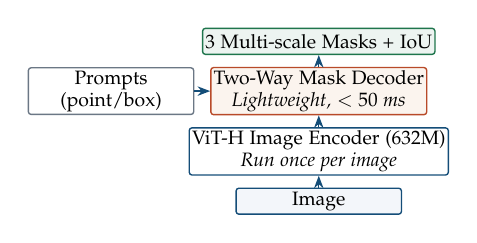
\begin{tikzpicture}[node distance=1.1mm,every node/.style={font=\scriptsize},
  bx/.style={box,minimum width=21mm,minimum height=3.3mm,inner sep=1pt}]
\node[bx,fill=soft] (img) {Image};
\node[bx,draw=acc,above=1.5mm of img] (enc) {ViT-H Image Encoder (632M)\\\emph{Run once per image}};
\node[bx,draw=acc2,fill=soft2,above=1.5mm of enc] (dec) {Two-Way Mask Decoder\\\emph{Lightweight, $<50\text{ ms}$}};
\node[bx,draw=mute,left=2mm of dec] (pr) {Prompts\\(point/box)};
\node[bx,draw=acc3,fill=acc3!8,above=1.5mm of dec] (mask) {3 Multi-scale Masks + IoU};
\draw[arr] (img)--(enc); \draw[arr] (enc)--(dec); \draw[arr] (pr)--(dec); \draw[arr] (dec)--(mask);
\end{tikzpicture}%
}
}{%
\textbf{The SAM Architecture.} Splits heavy perception from interactive decoding.\\[2pt]
{\color{acc2}$\blacktriangleright$} \textbf{Asymmetric design}: The heavy ViT image encoder produces a $64\times 64 \times 256$ spatial embedding once. Interactive clicks/prompts run purely through the sub-50ms decoder in real time.\\
{\color{acc2}$\blacktriangleright$} \textbf{Ambiguity awareness}: Predicts 3 valid hierarchy masks (whole, part, subpart) to handle ambiguous single-point clicks.
}

\begin{mem}[Segmentation Paradigms Compared]
\begin{tabularx}{\linewidth}{@{}p{17mm} X X@{}}
\toprule
\textbf{Task} & \textbf{Target Output} & \textbf{Canonical Benchmark}\\
\midrule
\textbf{Semantic} & Every pixel assigned class $c \in \{1,\dots,C\}$; no individual object separation. & ADE20K (mIoU), Cityscapes\\
\textbf{Instance} & Pixels grouped into discrete instance masks for "thing" categories (people, cars). & COCO Mask AP ($\text{AP}_{\text{mask}}$)\\
\textbf{Panoptic} & Unified: Instance masks for countable "things" $+$ semantic masks for amorphous "stuff" (sky, grass). & COCO Panoptic Quality ($\text{PQ} = \text{SQ} \times \text{RQ}$)\\
\bottomrule
\end{tabularx}
\end{mem}

\begin{qa}[Segmentation Mechanics \& Modern Foundation Models]
\Q{Why are U-Net skip connections necessary for precise biomedical and boundary segmentation?}{
Successive pooling and strided convolutions downsample feature maps to capture high-level semantic context, destroying fine spatial details and precise pixel locations.
\textbf{U-Net skip connections} concatenate shallow encoder features directly with decoder feature maps at the matching scale:
Decoder receives both:
\begin{enumerate}[leftmargin=*,itemsep=0.8pt]
\item Low-frequency semantic abstractions from the bottleneck.
\item High-frequency boundary and edge signals directly from the early encoder.
\end{enumerate}
Enables exact boundary localization without requiring dilated convolutions.}
\Q{How does DeepLabv3+ use Atrous Spatial Pyramid Pooling (ASPP) to capture multi-scale context?}{
Chen et al. address the trade-off between receptive field and feature resolution using atrous/dilated convolutions with rate $r$: $K' = K + (K-1)(r-1)$.
\textbf{ASPP Architecture}:
Processes incoming feature map $x$ in parallel through 5 branches:
\begin{enumerate}[leftmargin=*,itemsep=0.8pt]
\item One $1\times 1$ convolution (preserves local details).
\item Three $3\times 3$ atrous convolutions with rates $r = [6, 12, 18]$ (samples distant context without reducing resolution).
\item Image-level Global Average Pooling followed by $1\times 1$ conv and bilinear upsampling (captures global image prior).
\end{enumerate}
All branches are concatenated along channels and projected through a $1\times 1$ conv to produce multi-scale context representation.}
\Q{How does Mask2Former unify semantic, instance, and panoptic segmentation?}{
Cheng et al. discard task-specific heads (RoIAlign, FCN) in favor of \textbf{Masked-Attention Transformers}:
\begin{enumerate}[leftmargin=*,itemsep=0.8pt]
\item Employs $N$ object queries that predict binary mask logits $m_i \in [0, 1]^{H\times W}$ and class distribution $p_i$.
\item \textbf{Masked Attention}: Modulates decoder cross-attention to attend \emph{only} within the foreground area predicted by the previous layer's mask:
$$\mathcal{M}_{l-1}(x, y) = \begin{cases} 0 & \text{if } m_{l-1}(x, y) > 0.5 \\ -\infty & \text{otherwise} \end{cases}$$
Focuses attention on relevant localized object features, dramatically accelerating convergence and outperforming specialized models across all 3 tasks.
\end{enumerate}}
\Q{How does Mask R-CNN predict instance masks, and why a per-class sigmoid?}{
A third head runs on every positive RoI: RoIAlign to $14\times 14$, four $3\times 3$ convs, a $2\times$ deconv, then a $1\times 1$ conv giving $K$ masks of $28\times 28$ (one per class).
\textbf{Loss}: binary cross-entropy on the mask of the \emph{ground-truth class only}, $\mathcal{L} = \mathcal{L}_{\text{cls}} + \mathcal{L}_{\text{box}} + \mathcal{L}_{\text{mask}}$.\\
\textbf{Why decouple}: a per-pixel softmax over classes makes masks compete; the paper reports about $+5.5$ mask AP for per-class sigmoids, because the box head already decides the class.\\
\textbf{Inference}: take the mask for the predicted class, resize the $28\times 28$ map to the box, threshold at 0.5. The low $28^2$ resolution is why boundaries look blobby (PointRend and Mask2Former fix this).}
\end{qa}

\begin{trap}[Segmentation Metrics]
\begin{itemize}
\item \textbf{mIoU vs Pixel Accuracy}: Pixel accuracy is easily distorted by background dominance (predicting background on $95\%$ of pixels gives $95\%$ accuracy but near-zero mIoU). Always optimize and report mean Intersection-over-Union: $\text{mIoU} = \frac{1}{C} \sum_{c} \frac{TP_c}{TP_c + FP_c + FN_c}$.
\item \textbf{Dice Loss gradient near empty masks}: $\text{Dice} = \frac{2 |X \cap Y| + \epsilon}{|X| + |Y| + \epsilon}$. If $\epsilon$ is too small ($< 10^{-7}$), division by tiny denominator when both prediction and ground truth are empty yields numerical instability.
\end{itemize}
\end{trap}

\section{Foundation Segmentation: SAM \& SAM 2}\label{sec:sam}
\lab{SAM ViT-H \textperiodcentered\ prompt encoder \textperiodcentered\ two-way decoder \textperiodcentered\ ambiguity resolution \textperiodcentered\ SAM 2 streaming video \textperiodcentered\ memory bank}

\begin{mem}[SAM vs SAM 2 Architecture Comparison]
\begin{tabularx}{\columnwidth}{@{}l X X@{}}
\toprule
\textbf{Component} & \textbf{SAM (Images, 2023)} & \textbf{SAM 2 (Images \& Videos, 2024)} \\
\midrule
\textbf{Image Backbone} & ViT-H/L/B (MAE pretrained, $1024\times 1024$, windowed attn) & Hiera hierarchical backbone (multiscale, faster execution) \\
\textbf{Prompt Types} & Points (pos/neg), bounding boxes, dense masks & Points, boxes, masks across any video timestep \\
\textbf{Decoder} & Two-way cross-attention transformer (prompt $\leftrightarrow$ image) & Two-way transformer + Occlusion prediction head \\
\textbf{Temporal State} & None (single static frame) & Streaming Memory Bank (FIFO past frames + prompted frames) \\
\textbf{Memory Attention} & N/A & L-layer cross-attention attending to stored memory features \\
\textbf{Dataset} & SA-1B (11M images, 1.1B masks) & SA-V (51k videos, 600k masklets, $53\times$ more masks than prior) \\
\bottomrule
\end{tabularx}
\end{mem}

\begin{qa}[Segment Anything (SAM) Deep Dive]
\Q{How does the SAM architecture decouple the heavy image encoder from the real-time prompt decoder?}{
\textbf{Decoupled Design}:
\begin{enumerate}
\item \textbf{Image Encoder (Heavyweight)}: Uses ViT-H (632M parameters) with input resolution $1024 \times 1024$. To avoid quadratic self-attention cost across all $64 \times 64 = 4096$ patches, it uses interleaved local window attention with only 4 global attention blocks.
Image encoding takes $\sim 450$\,ms on an A100 GPU, but runs \hl{exactly once} per image to output a spatial feature embedding $\mathbf{F} \in \mathbb{R}^{64 \times 64 \times 256}$.
\item \textbf{Prompt Encoder (Lightweight)}:
\begin{itemize}
\item \textbf{Sparse prompts (Points/Boxes)}: Point $(x, y)$ is represented by 2D Fourier positional encoding plus learned embeddings indicating point type (foreground vs background). Bounding boxes are encoded as two points (top-left and bottom-right).
\item \textbf{Dense prompts (Masks)}: Downsampled via convolutional layers and element-wise added to the image embedding.
\end{itemize}
\item \textbf{Mask Decoder (Real-time)}: A tiny two-way transformer ($\sim 4$\,M parameters). Prompt tokens attend to image embeddings, and image embeddings attend to prompt tokens.
Decodes in $<50$\,ms on modern GPUs, enabling instant, fluid interactive browser annotation.
\end{enumerate}}

\Q{How does SAM solve the mathematical ambiguity of a single point prompt without collapsing training gradients?}{
\textbf{The Ambiguity Problem}: A single click on an person's shirt could mean (1) the shirt button, (2) the shirt itself, or (3) the entire person. Training a standard network with binary cross-entropy on ground-truth masks produces blurry, averaged probabilities that attempt to satisfy all three meanings simultaneously.\\[2pt]
\textbf{SAM Ambiguity Resolution}:
\begin{itemize}
\item The mask decoder always outputs \hl{3 distinct mask tokens} simultaneously, representing subpart, part, and whole object.
\item During training, SAM calculates the loss against ground-truth for all 3 masks, but backpropagates gradients \hl{only through the single mask with the lowest loss} (minimum error backpropagation).
\item In addition, an auxiliary MLP head predicts the IoU score for each mask.
\item At inference, if ambiguous, SAM displays the 3 candidate masks or selects the one with the highest predicted IoU score.
\end{itemize}}
\end{qa}

\begin{qa}[SAM 2: Video Object Segmentation \& Memory Dynamics]
\Q{How does SAM 2 extend promptable segmentation to continuous video streams in real time?}{
SAM 2 introduces a causal streaming architecture that processes video frame-by-frame:
\begin{itemize}
\item \textbf{Memory Attention Block}: When a new frame $t$ arrives, its Hiera visual features attend to previous spatial-temporal representations stored in the \textbf{Memory Bank} via stacked cross-attention layers.
\item \textbf{Streaming Memory Bank}: Stores two distinct types of memories:
\begin{enumerate}
\item \textbf{Temporal FIFO}: A sliding window of features from the most recent $N$ frames (capturing immediate motion and appearance transitions).
\item \textbf{Prompted Anchors}: Features from all frames where the user provided explicit interactive prompts (preventing catastrophic forgetting and drift over long videos).
\end{enumerate}
\item \textbf{Memory Encoder}: Once a mask is predicted for frame $t$, a lightweight convolutional memory encoder downsamples the mask, fuses it with image features, and writes the compact embedding into the memory bank.
\item \textbf{Occlusion Head}: Predicts a probability $p_{\text{occ}} \in [0, 1]$ indicating whether the target object is currently visible. If occluded, the memory bank suppresses visual updates to avoid contaminating tracking with background clutter.
\end{itemize}}

\Q{Why did SAM 2 replace the ViT backbone with Hiera, and what is the latency advantage?}{
\textbf{ViT-H limitations}: Standard ViT operates at a single fixed scale with isotropic resolution, requiring costly windowed attention and large FLOP budgets ($\sim 632$M parameters, $\sim 50$ms per frame even after caching).\\[2pt]
\textbf{Hiera Backbone}: A hierarchical vision transformer that produces multi-scale feature maps ($4\times, 8\times, 16\times, 32\times$) with simple masked autoencoder pretraining. It removes complex operations (no shifted windows, no relative position bias tables, no multi-path branches) and relies purely on simple spatial pooling.
Result: SAM 2 achieves \hl{$6\times$ faster runtime} ($44$ FPS on A100 vs $7$ FPS for SAM), enabling true real-time video tracking.}
\end{qa}

\begin{trap}[SAM / SAM 2 Practical Traps]
\begin{itemize}
\item \textbf{Semantic Class Agnosticism}: SAM predicts \emph{masks}, not semantic \emph{categories}. It outputs "where" an object is, but has zero awareness of "what" it is. For semantic segmentation, SAM must be paired with CLIP/Grounding-DINO.
\item \textbf{Memory Bank GPU Leak in SAM 2}: In long videos ($>1000$ frames), an unbounded memory bank exhausts GPU VRAM. In production streaming, enforce strict FIFO eviction capping unprompted history to $N=8$ frames.
\end{itemize}
\end{trap}

\section{Self-Supervised Vision: Contrastive, MAE \& DINOv2}\label{sec:ssl}
\lab{SimCLR \textperiodcentered\ MoCo v1-v3 \textperiodcentered\ BYOL \textperiodcentered\ MAE \textperiodcentered\ DINO \textperiodcentered\ DINOv2 \textperiodcentered\ KoLeo}

\noindent\begin{minipage}[t]{0.42\columnwidth}\vspace{0pt}\centering
\resizebox{\linewidth}{!}{%
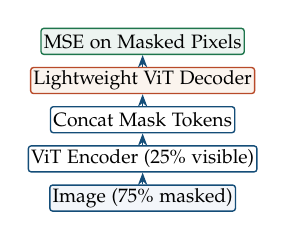
\begin{tikzpicture}[node distance=1.1mm,every node/.style={font=\tiny},
  bx/.style={box,minimum width=21mm,minimum height=3.3mm,inner sep=1pt}]
\node[bx,fill=soft] (img) {Image ($75\%\text{ masked}$)};
\node[bx,draw=acc,above=1.5mm of img] (enc) {ViT Encoder ($25\%\text{ visible}$)};
\node[bx,above=1.5mm of enc] (cat) {Concat Mask Tokens};
\node[bx,draw=acc2,fill=soft2,above=1.5mm of cat] (dec) {Lightweight ViT Decoder};
\node[bx,draw=acc3,fill=acc3!8,above=1.5mm of dec] (loss) {MSE on Masked Pixels};
\draw[arr] (img)--(enc); \draw[arr] (enc)--(cat); \draw[arr] (cat)--(dec); \draw[arr] (dec)--(loss);
\end{tikzpicture}%
}
\end{minipage}\hfill
\begin{minipage}[t]{0.56\columnwidth}\vspace{1pt}\small
\textbf{The MAE Paradigm.} Exploits heavy 2D pixel redundancy.\\[2pt]
{\color{acc2}$\blacktriangleright$} \textbf{Asymmetric architecture}: Only the $25\%$ unmasked patches pass through the heavy encoder. The shallow decoder reconstructs normalized pixels.\\[2pt]
{\color{acc2}$\blacktriangleright$} \textbf{Speedup}: $4\times$ compute reduction and memory savings during pretraining compared to standard ViT.
\end{minipage}

\begin{mem}[SSL Vision Paradigms Comparison]
\begin{tabularx}{\linewidth}{@{}p{18mm} X X@{}}
\toprule
\textbf{Method} & \textbf{Core Loss / Objective} & \textbf{Collapse Prevention Mechanism}\\
\midrule
\textbf{SimCLR} & InfoNCE with negative pairs across batch & Massive batch size ($B=4096$) + non-linear projection head.\\
\textbf{MoCo v1--v3} & InfoNCE over persistent memory queue & Momentum-updated key encoder ($\theta_k \leftarrow m\theta_k + (1-m)\theta_q$).\\
\textbf{BYOL / SimSiam} & MSE between online predictor and target & \textbf{Stop-gradient} ($\text{sg}[\cdot]$) on target branch + asymmetric predictor MLP.\\
\textbf{MAE} & Pixel MSE on masked patches & Reconstruction task (no negative pairs; cannot collapse to constant).\\
\textbf{DINO / DINOv2} & Cross-entropy student vs momentum teacher & Logit \textbf{centering} (prevents 1-class mode) $+$ \textbf{sharpening} (prevents uniform mode).\\
\bottomrule
\end{tabularx}
\end{mem}

\begin{qa}[Self-Supervised Mechanics \& Representation Geometry]
\Q{Derive why InfoNCE minimizes the lower bound on Mutual Information $I(X; Y)$.}{
Let $(x, y)$ be positive pairs and $\{y_k^-\}_{k=1}^K$ be $K$ negative samples drawn from marginal $p(y)$.
The InfoNCE loss is:
$$\mathcal{L}_{\text{InfoNCE}} = -\mathbb{E}\left[ \log \frac{e^{f(x, y)}}{\sum_{k=1}^K e^{f(x, y_k)}} \right]$$
By Jensen's inequality and properties of Bayes' rule:
\begin{align*}
\mathcal{L}_{\text{InfoNCE}} &\ge \mathbb{E}\left[ \log \left( 1 + (K-1) \frac{p(y)}{p(y|x)} \right) \right]\\
&\approx \log(K) - I(X; Y) \implies I(X; Y) \ge \log(K) - \mathcal{L}_{\text{InfoNCE}}
\end{align*}
Minimizing InfoNCE maximizes the mutual information lower bound between augmented views. Larger batch/queue size $K$ directly tightens the bound $\log(K)$.}
\Q{Why does MAE mask 75\% of visual patches, whereas BERT masks only 15\% of words?}{
\textbf{Information Density}: Language is human-generated, highly symbolic, and dense with semantics: masking more than $15\%$ destroys grammar and syntactic recoverability.
Images are natural signals with extreme spatial correlation: adjacent pixels and patches share nearly identical color, lighting, and texture.
Masking only $15-20\%$ allows the network to interpolate masked patches trivially from neighboring borders without understanding high-level 3D structure or semantics.
A $75-80\%$ mask removes entire objects and context, forcing the encoder to learn holistic geometric representations.}
\Q{How does DINO produce emergent semantic segmentation without annotations?}{
Caron et al. train a ViT student to match a momentum teacher over multi-crop views.
Because the objective maximizes agreement between global crops (full image) and local crops (sub-regions), and because self-attention in transformers connects all spatial tokens without local receptive field restrictions:
The \texttt{[CLS]} and patch tokens learn to cluster around distinct foreground objects to maximize mutual information across varied scales.
Attention maps from the last layer of DINO explicitly outline foreground objects without any segmentation labels or bounding boxes.}
\Q{What makes DINOv2 the gold-standard frozen vision feature extractor?}{
Oquab et al. scale self-distillation to 1B parameters (ViT-g):
\begin{enumerate}[leftmargin=*,itemsep=0.8pt]
\item \textbf{Curated LVD-142M Data Pipeline}: De-duplicates, filters, and balances 142M images using nearest-neighbor embedding retrieval against ImageNet-22k.
\item \textbf{Joint iBOT Objective}: Applies token-level masked image modeling simultaneously with view-level DINO self-distillation.
\item \textbf{KoLeo Regularizer}: Adds Kozachenko-Leonenko differential entropy estimator minimizing $-\sum_{i} \log \min_{j \ne i} \|z_i - z_j\|_2$, forcing visual feature embeddings to spread uniformly over the unit hypersphere.
\end{enumerate}
Freezing DINOv2 features outperforms weakly supervised models on zero-shot classification, monocular depth estimation, and dense feature matching.}
\end{qa}

\begin{trap}[SSL Pretraining Traps]
\begin{itemize}
\item \textbf{Discarding the projection head}: In SimCLR, MoCo, and BYOL, downstream evaluation must use the encoder representation $h = f(x)$, \textbf{not} the projection head output $z = g(h)$. The projection head discards information (e.g., color, orientation) irrelevant to the contrastive objective that is vital for downstream tasks.
\item \textbf{Patch norm in MAE}: Reconstructing raw RGB pixels directly causes the model to focus on low-frequency lighting shifts. Computing target pixel values normalized by the mean and variance of each patch ($y = (x - \mu) / \sigma$) gains $+1.5\%$ top-1 accuracy.
\end{itemize}
\end{trap}

\section{SSL Deep Dive: MAE, DINO \& DINOv2}\label{sec:ssl-deep}
\lab{MAE asymmetric encoder \textperiodcentered\ 75\% masking \textperiodcentered\ DINO centering \& sharpening \textperiodcentered\ KoLeo regularizer \textperiodcentered\ Register tokens}

\begin{mem}[MAE vs DINOv2 Paradigm Comparison]
\begin{tabularx}{\columnwidth}{@{}p{19mm} X X@{}}
\toprule
\textbf{Property} & \textbf{Masked Autoencoders (MAE)} & \textbf{Self-Distillation (DINOv2)} \\
\midrule
\textbf{Objective} & Reconstruct masked pixels ($L_2$ MSE) & Match teacher probability distribution (Cross-Entropy) \\
\textbf{Supervision} & Generative reconstruction & Joint embedding self-distillation \\
\textbf{Masking / Views} & $75\%$ random masking of patches & Multi-crop (2 global views + 8 local views) \\
\textbf{Asymmetry} & Encoder sees only $25\%$ visible patches & Student sees local+global; Teacher sees global only \\
\textbf{Features} & Strong fine-tuning backbone; poor k-NN & State-of-the-art frozen features; $>86\%$ linear probe \\
\textbf{Regularizer} & Normalized patch pixel targets & KoLeo differential entropy + Register tokens \\
\bottomrule
\end{tabularx}
\end{mem}

\begin{qa}[Masked Autoencoders (MAE) Mechanics]
\Q{Why does MAE mask 75\% of image patches, whereas BERT masks only 15\% of text tokens?}{
\textbf{Information Density}: Language is highly information-dense, discrete, and semantic; masking $15\%$ of words in a sentence already leaves subtle, challenging cloze puzzles. In contrast, images are continuous, spatially redundant signals: adjacent pixels are heavily correlated.
\begin{itemize}
\item At $15\%$ image masking, a network can reconstruct missing pixels through trivial local spatial interpolation (blurring/edge continuation) without understanding high-level scene composition.
\item At \hl{$75\%$ masking}, only $1$ in $4$ patches is visible. The model cannot interpolate locally; it is forced to learn holistic scene grammar (e.g., inferring that an eye requires a nose, mouth, and face).
\end{itemize}}

\Q{How does MAE achieve a 4x throughput acceleration during pretraining?}{
\textbf{Asymmetric Architecture}:
\begin{enumerate}
\item \textbf{Heavy Encoder}: Operates \hl{strictly on visible patches}. For $196$ total patches, $75\%$ masking leaves only $N_{\text{vis}} = 49$ tokens. Since ViT self-attention scales quadratically, attention FLOPs drop by $\left(\frac{49}{196}\right)^2 = \left(\frac{1}{4}\right)^2 = \mathbf{\frac{1}{16}}$!
\item \textbf{Lightweight Decoder}: Only after the heavy encoder has processed visible tokens are learned, shared [mask] tokens inserted at the masked positions to form the complete $196$-token sequence. The decoder is shallow ($\sim 8$ layers vs $24$ in encoder), incurring minimal compute.
\item \textbf{Loss Computation}: MSE is computed \hl{only on masked patches}, further saving loss evaluation overhead.
\end{enumerate}}
\end{qa}

\begin{qa}[DINO \& DINOv2 Self-Distillation Dynamics]
\Q{Derive how DINO avoids representation collapse without negative pairs via Centering and Sharpening.}{
In self-distillation, student $g_s$ predicts teacher $g_t$ output. Two failure modes (collapse) threaten training:
\begin{enumerate}
\item \textbf{Dirac collapse}: Output distribution collapses to a single constant coordinate for all inputs.
\item \textbf{Uniform collapse}: Output distribution collapses to a uniform distribution with maximum entropy.
\end{enumerate}
DINO parameterizes probability outputs via temperatures $\tau_s, \tau_t$ and center vector $c$:
\begin{align*}
P_s(x)^{(i)} &= \frac{\exp(g_s(x)^{(i)} / \tau_s)}{\sum_k \exp(g_s(x)^{(k)} / \tau_s)}\\
P_t(x)^{(i)} &= \frac{\exp((g_t(x)^{(i)} - c_i) / \tau_t)}{\sum_k \exp((g_t(x)^{(k)} - c_k) / \tau_t)}
\end{align*}
\begin{itemize}
\item \textbf{Centering}: $c \leftarrow m \cdot c + (1-m) \frac{1}{B}\sum_{b} g_t(x_b)$. Subtracting the center vector pulls the mean activation toward zero, preventing any single dimension from dominating (averts Dirac collapse). However, excessive centering pushes probabilities toward uniform distribution.
\item \textbf{Sharpening}: Setting teacher temperature $\tau_t < \tau_s$ ($\tau_t \approx 0.04-0.07$ vs $\tau_s \approx 0.1$) sharpens the distribution, counteracting the uniform dispersion.
\item \textbf{Equilibrium}: Centering and sharpening act as opposing forces: centering pushes toward uniform entropy, sharpening pushes toward peaked entropy. Balanced together, they guarantee stable non-collapsed representations.
\end{itemize}}

\Q{What is the KoLeo regularizer in DINOv2, and how do Register Tokens eliminate feature map artifacts?}{
\textbf{KoLeo (Kozachenko-Leonenko) Regularizer}:
Computes an empirical estimate of differential entropy across normalized feature vectors $z_i$:
$$\mathcal{L}_{\text{KoLeo}} = - \frac{1}{n} \sum_{i=1}^n \ln \left( \min_{j \ne i} \| z_i - z_j \|_2 \right)$$
Minimizing $\mathcal{L}_{\text{KoLeo}}$ maximizes the distance between every feature vector and its nearest neighbor, forcing representations to distribute uniformly across the unit hypersphere and preventing feature clustering.\\[2pt]
\textbf{Register Tokens (Darcet et al., 2023)}:
Standard ViTs trained with DINO/DINOv2 exhibit severe high-norm spike artifacts in flat, uniform background regions (5x higher activation norms than foreground objects).
\begin{itemize}
\item \textbf{Cause}: Because ViT lacks dedicated scratchpad memory, self-attention recycles uninformative background tokens to store global contextual information.
\item \textbf{Solution}: Append 4--8 learnable [register] tokens to the input patch sequence. The model automatically routes global context through registers, completely eliminating background visual artifacts and producing razor-sharp feature maps.
\end{itemize}}
\end{qa}

\begin{trap}[SSL Pretraining Traps]
\begin{itemize}
\item \textbf{Patch Pixel Normalization in MAE}: Omitting per-patch mean/variance normalization ($\frac{x - \mu}{\sigma}$) when computing MAE reconstruction loss costs about 3 points of linear-probe accuracy (68.0 $\to$ 64.8 for ViT-L), as the model wastes capacity fitting global illumination variations rather than local structural geometry.
\item \textbf{EMA Teacher Update Rate}: The teacher EMA momentum must start high ($\lambda = 0.996$) and cosine-anneal to $1.0$ at the end of training. Setting $\lambda$ too low makes the teacher track noisy student weights, destabilizing training.
\end{itemize}
\end{trap}

\section{Vision-Language Foundations: CLIP to SigLIP}\label{sec:clip}
\lab{CLIP \textperiodcentered\ dual encoder \textperiodcentered\ InfoNCE \textperiodcentered\ SigLIP sigmoid loss \textperiodcentered\ zero-shot transfer \textperiodcentered\ all-gather}

\noindent\begin{minipage}[t]{0.42\columnwidth}\vspace{0pt}\centering
\resizebox{\linewidth}{!}{%
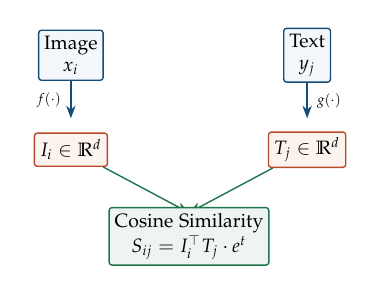
\begin{tikzpicture}[x=1mm,y=1mm,every node/.style={font=\tiny}]
\node[box,draw=acc,fill=soft] (img) at (0,14) {Image\\$x_i$};
\node[box,draw=acc,fill=soft] (txt) at (30,14) {Text\\$y_j$};
\draw[arr] (img) -- (0,6) node[midway,left] {$f(\cdot)$};
\draw[arr] (txt) -- (30,6) node[midway,right] {$g(\cdot)$};
\node[box,draw=acc2,fill=soft2] (ie) at (0,2) {$I_i \in \mathbb{R}^d$};
\node[box,draw=acc2,fill=soft2] (te) at (30,2) {$T_j \in \mathbb{R}^d$};
\draw[arr,acc3] (ie) -- (15,-6);
\draw[arr,acc3] (te) -- (15,-6);
\node[box,draw=acc3,fill=acc3!8] (sim) at (15,-9) {Cosine Similarity\\$S_{ij} = I_i^\top T_j \cdot e^t$};
\end{tikzpicture}%
}
\end{minipage}\hfill
\begin{minipage}[t]{0.56\columnwidth}\vspace{1pt}\small
\textbf{The Dual-Encoder Contrastive Setup.} Embeds images and text into a shared normalized latent space $\mathbb{R}^d$ ($d=512$ or $768$).\\[2pt]
{\color{acc2}$\blacktriangleright$} \textbf{Zero-Shot Transfer}: Candidate class names embedded with prompt template $\to$ cosine similarity $\to$ argmax class.\\[2pt]
{\color{acc2}$\blacktriangleright$} \textbf{Temperature clamping}: Learned log-temperature $t$ clamped to $\le \ln(100) \approx 4.605$ to prevent softmax saturation and numerical blowup.
\end{minipage}

\begin{mem}[Loss Formulations: CLIP vs SigLIP]
\begin{itemize}
\item \textbf{CLIP (Symmetric InfoNCE)}: Computes cross-entropy over batch $B$:
$$\mathcal{L}_{\text{CLIP}} = -\frac{1}{2B} \sum_{i=1}^B \left( \log \frac{e^{S_{ii}}}{\sum_{j=1}^B e^{S_{ij}}} + \log \frac{e^{S_{ii}}}{\sum_{j=1}^B e^{S_{ji}}} \right)$$
Requires all-gather communication across all GPUs to form the global denominator; communication cost $\mathcal{O}(B^2)$ bounds maximum batch size.
\item \textbf{SigLIP (Sigmoid Loss)}: Formulates language-image alignment as pairwise binary classification:
$$\mathcal{L}_{\text{SigLIP}} = -\frac{1}{B} \sum_{i=1}^B \sum_{j=1}^B \log \sigma\left( y_{ij} (I_i^\top T_j \cdot e^t + b) \right)$$
where $y_{ij} = +1$ if $i=j$, else $-1$. Eliminates global softmax normalization; enables chunked loss computation and seamless scaling to batch sizes $B > 1\text{M}$.
\end{itemize}
\end{mem}

\begin{qa}[Contrastive Multimodal Mechanics \& Communication Scaling]
\Q{Derive the gradient of the InfoNCE loss with respect to similarity logits $S_{ij}$.}{
For a single sample $i$, the image-to-text loss is $\mathcal{L}_i = -\log p_{ii}$ where $p_{ij} = \frac{e^{S_{ij}}}{\sum_k e^{S_{ik}}}$.
Differentiating with respect to logit $S_{ij}$:
$$\frac{\partial \mathcal{L}_i}{\partial S_{ij}} = p_{ij} - y_{ij} \quad \text{where } y_{ij} = \mathbf{1}_{\{i = j\}}$$
\begin{itemize}
\item For the positive target ($j=i$): $\frac{\partial \mathcal{L}_i}{\partial S_{ii}} = p_{ii} - 1 < 0$ (pulls positive similarity upward).
\item For negative targets ($j \ne i$): $\frac{\partial \mathcal{L}_i}{\partial S_{ij}} = p_{ij} > 0$ (pushes negative similarity downward proportional to its current probability mass).
\end{itemize}
Softmax creates competition: pushing up the positive logit suppresses all negatives simultaneously, but requires summing over all negatives in the denominator.}
\Q{Why does SigLIP scale to $10\times$ larger batch sizes than CLIP in distributed clusters?}{
In standard CLIP, computing $\sum_{j=1}^B e^{S_{ij}}$ requires every GPU to know the embeddings of all $B$ images and texts across the entire cluster.
In distributed data parallel (DDP) across $N$ GPUs, this necessitates an \textbf{All-Gather} collective communication operation of all embedding tensors ($2 \times B \times d$).
At $B=65{,}536$, the all-gather payload and quadratic attention matrix $B\times B$ saturate GPU interconnect bandwidth (NVLink/Infiniband).
\textbf{SigLIP Solution}: Binary classification evaluates independent pairs $(i, j)$ without a global partition function.
Embeddings can be sharded and evaluated in streaming pipeline chunks: each GPU computes local dot products and loss without ever gathering the global batch, enabling linear scaling up to $B=1\text{M}$ with $+1.5\%$ higher zero-shot accuracy.}
\Q{Why is zero-shot CLIP significantly more robust to distribution shift than supervised ImageNet models?}{
Supervised ResNet models learn shortcut features (high-frequency background textures, camera color balances, specific noise profiles) correlated with ImageNet labels.
When tested on shifted distributions (ImageNet-A adversarial examples, ImageNet-R art/sketches, ImageNet-C corruptions), supervised accuracy drops precipitously ($\sim 40\%$ drop).
CLIP is pretrained on 400M diverse internet image-caption pairs using natural language supervision:
It learns invariant semantic concepts (e.g., "whiskers", "four legs", "stripes") rather than single-dataset statistical artifacts.
On distribution-shifted benchmarks, CLIP retains up to $20-30\%$ higher accuracy than supervised equivalents with identical ImageNet-1K top-1 accuracy.}
\end{qa}

\begin{trap}[Dual Encoder Pitfalls]
\begin{itemize}
\item \textbf{L2 Normalization before dot product}: Both visual embeddings $I$ and text embeddings $T$ \textbf{must} be L2-normalized ($\|I\|_2 = 1, \|T\|_2 = 1$) before the dot product and temperature scaling. Omitting normalization breaks the cosine geometry, allowing outlier vector lengths to dominate the loss.
\item \textbf{Prompt sensitivity}: Evaluating single-word class names ("dog") yields $5-10\%$ lower zero-shot accuracy than prompt ensembles (averaging embeddings of 80 templates: "a photo of a {label}", "a close-up of the {label}").
\end{itemize}
\end{trap}

\section{Multimodal LLMs: Architecture, AnyRes \& Alignment}\label{sec:vlm}
\lab{LLaVA \textperiodcentered\ Projectors \textperiodcentered\ AnyRes dynamic resolution \textperiodcentered\ 2D RoPE \textperiodcentered\ Qwen2-VL \textperiodcentered\ Hallucination \& POPE}

\noindent\begin{minipage}[t]{0.42\columnwidth}\vspace{0pt}\centering
\resizebox{\linewidth}{!}{%
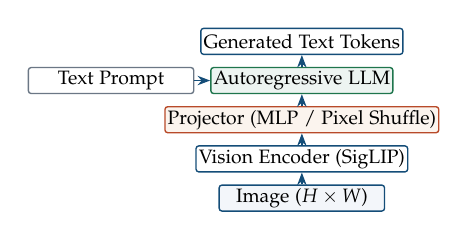
\begin{tikzpicture}[node distance=1.1mm,every node/.style={font=\tiny},
  bx/.style={box,minimum width=21mm,minimum height=3.3mm,inner sep=1pt}]
\node[bx,fill=soft] (img) {Image ($H\times W$)};
\node[bx,draw=acc,above=1.5mm of img] (enc) {Vision Encoder (SigLIP)};
\node[bx,draw=acc2,fill=soft2,above=1.5mm of enc] (proj) {Projector (MLP / Pixel Shuffle)};
\node[bx,draw=acc3,fill=acc3!8,above=1.5mm of proj] (llm) {Autoregressive LLM};
\node[bx,above=1.5mm of llm] (out) {Generated Text Tokens};
\draw[arr] (img)--(enc); \draw[arr] (enc)--(proj); \draw[arr] (proj)--(llm); \draw[arr] (llm)--(out);
\node[bx,draw=mute,left=2mm of llm] (txt) {Text Prompt};
\draw[arr] (txt)--(llm);
\end{tikzpicture}%
}
\end{minipage}\hfill
\begin{minipage}[t]{0.56\columnwidth}\vspace{1pt}\small
\textbf{The Modern VLM Pipeline.} Integrates visual tokens directly into the LLM's sequence context.\\[2pt]
{\color{acc2}$\blacktriangleright$} \textbf{Token budget}: A $336\times 336$ image with patch 14 produces $(336/14)^2 = 576$ visual tokens.\\
{\color{acc2}$\blacktriangleright$} \textbf{Pixel Shuffle}: Merging $2\times 2$ adjacent patch tokens compresses sequence length by $4\times$ ($576 \to 144$ tokens), preserving LLM context budget.
\end{minipage}

\begin{mem}[Visual Connectors / Projectors]
\begin{tabularx}{\linewidth}{@{}p{22mm} X X@{}}
\toprule
\textbf{Connector} & \textbf{Mechanism} & \textbf{Trade-off}\\
\midrule
\textbf{Linear / 2-Layer MLP} (LLaVA) & $H_v = W_2 \cdot \text{GELU}(W_1 \cdot Z_v)$ & Preserves spatial topology 1:1; high token count in LLM context.\\
\textbf{Perceiver / Q-Former} (BLIP-2) & $K$ learned query tokens cross-attend to visual features & Compresses visual sequence to fixed size (e.g. 64); loses fine-grained dense OCR details.\\
\textbf{Pixel Shuffle / Merge} (InternVL, Qwen2) & Reshapes $2\times 2$ spatial tokens into channels: $(H/2, W/2, 4C) \to (H/2, W/2, C_{\text{LLM}})$ & $4\times$ token reduction while maintaining 2D spatial relative geometry.\\
\bottomrule
\end{tabularx}
\end{mem}

\begin{qa}[High-Resolution \& Alignment]
\Q{How does the AnyRes (grid slicing) strategy handle high-resolution documents and charts?}{
Standard ViTs downsample images to fixed small resolutions (e.g., $336\times 336$), rendering small text and chart labels unreadable.
\textbf{AnyRes Strategy (LLaVA-NeXT)}:
\begin{enumerate}[leftmargin=*,itemsep=0.8pt]
\item Determines an optimal grid of tiles (e.g., $1\times 2, 2\times 2, 1\times 3$) based on image aspect ratio.
\item Crops image into $N$ standard $336\times 336$ high-resolution patches, plus one downsampled global image for macro context.
\item Feeds all $N+1$ tiles through the ViT encoder independently.
\item Inserts special separator tokens (\texttt{<newline>}) between rows to maintain 2D layout semantics when flattened into the 1D LLM token sequence.
\end{enumerate}
Increases effective resolution up to $4\times$ while reusing pretrained small-resolution ViT weights.}
\Q{How does Qwen2-VL implement native dynamic resolution with 2D Rotary Position Embeddings?}{
Rather than slicing images into discrete artificial tiles, Qwen2-VL introduces a \textbf{Naive ViT} architecture:
\begin{itemize}[leftmargin=*,itemsep=0.8pt]
\item \textbf{Dynamic Patchification}: An image of arbitrary resolution $(H, W)$ is directly partitioned into $\frac{H}{14} \times \frac{W}{14}$ patches without padding or interpolation.
\item \textbf{2D RoPE (Rotary Position Embeddings)}: Query and key vectors at spatial coordinate $(x, y)$ are rotated by two independent 1D frequency angles:
$$\mathbf{R}_{2\text{D}}(x, y) = \text{diag}\big(\mathbf{R}(x), \mathbf{R}(y)\big)$$
Inner products $\langle \mathbf{q}_{(x_1, y_1)}, \mathbf{k}_{(x_2, y_2)} \rangle$ depend strictly on relative spatial distance $(\Delta x, \Delta y) = (x_1 - x_2, y_1 - y_2)$.
\item \textbf{Video Unification}: Replaces 2D RoPE with 3D RoPE $(t, x, y)$ to treat images and video frames within the exact same pipeline.
\end{itemize}
Eliminates tile boundaries and aspect ratio distortion completely.}
\Q{What causes object hallucination in VLMs, and how is it measured and mitigated?}{
\textbf{Cause}: Language priors overpower visual attention. Because the LLM backbone was pretrained on trillions of text tokens, strong statistical associations (e.g., "refrigerator" co-occurring with "kitchen", or "helmet" with "motorcycle") cause the model to generate tokens regardless of visual evidence.
\textbf{Measurement}: The \textbf{POPE (Polling-based Object Probing Evaluation)} benchmark queries whether specific objects exist in an image via binary yes/no questions under random, popular, and adversarial negative sampling.
\textbf{Mitigations}:
\begin{enumerate}[leftmargin=*,itemsep=0.8pt]
\item \textbf{DPO-V}: Direct preference optimization where hallucinated answers are marked as rejected pairs.
\item \textbf{Visual Contrastive Decoding (VCD)}: Samples from logits conditioned on clean image vs distorted/blurred image:
$$\text{logit}^* = (1+\alpha) \cdot \text{logit}(x) - \alpha \cdot \text{logit}(x_{\text{blurred}})$$
suppressing pure language prior biases and improving POPE score by $+8.5$ points.
\end{enumerate}}
\end{qa}

\begin{trap}[Multimodal Training Pitfalls]
\begin{itemize}
\item \textbf{Unfreezing vision encoder too early}: Unfreezing the vision encoder during Stage 1 (feature alignment) with random MLP projector weights corrupts the pretrained visual representations. Stage 1 must train \textbf{only} the projector.
\item \textbf{Loss masking}: Next-token cross-entropy loss must be computed \textbf{only} on the assistant's generated text tokens. Labels for user prompt text and visual tokens must be masked to $-100$ (\texttt{ignore\_index}).
\end{itemize}
\end{trap}

\section{VLM Evaluation \& Visual Hallucination}\label{sec:vlm-eval}
\lab{POPE benchmark \textperiodcentered\ affirmative bias \textperiodcentered\ Visual Contrastive Decoding (VCD) \textperiodcentered\ MMMU \textperiodcentered\ DocVQA \textperiodcentered\ OCR}

\begin{mem}[Key Vision-Language Benchmarks to Memorize]
\begin{tabularx}{\columnwidth}{@{}p{16mm} p{24mm} X@{}}
\toprule
\textbf{Benchmark} & \textbf{Evaluation Focus} & \textbf{Core Challenge / Metric} \\
\midrule
\textbf{POPE} & Object hallucination & Random, Popular, Adversarial; F1 \& Yes-ratio \\
\textbf{MMMU} & College reasoning & 30 subjects, diagrams, physics, schematics \\
\textbf{MathVista} & Visual math reasoning & Geometry proofs, coordinate plots, arithmetic \\
\textbf{DocVQA} & Document comprehension & Fine-grained OCR, invoice tables, font parsing \\
\textbf{ChartQA} & Data visualization & Numerical reasoning over bar charts, scatter plots \\
\textbf{MME} & Perception \& cognition & Yes/No probing with circular evaluation \\
\bottomrule
\end{tabularx}
\end{mem}

\begin{qa}[The POPE Benchmark \& Object Hallucination Mechanics]
\Q{How does POPE (Polling-based Object Probing Evaluation) expose visual hallucination, and what are its 3 splits?}{
Standard open-ended captioning metrics (CIDEr, BLEU) fail to detect hallucinations: a model can produce a beautifully fluent caption with $90\%$ true text and casually invent a dog or chair.\\[2pt]
\textbf{POPE Probing Format}: Converts object existence into binary Yes/No queries: \emph{"Is there a <object> in the image?"}
\begin{itemize}
\item \textbf{Random Split}: Queries non-existing objects selected purely at random from the dataset lexicon. (Tests baseline vocabulary discrimination).
\item \textbf{Popular Split}: Queries non-existing objects chosen from the most frequent objects in the dataset (e.g., person, car, chair). Exposes frequency bias where models hallucinate popular classes.
\item \textbf{Adversarial Split}: Queries non-existing objects that frequently \hl{co-occur} with objects actually present in the image. (e.g., an image contains a laptop; POPE queries whether a mouse is present). Tests whether the model looks at visual evidence or blindly relies on statistical text priors.
\end{itemize}
\textbf{Yes-Ratio Diagnostic}: A model reporting $80\%$ accuracy might have a $95\%$ "Yes" response rate; checking Precision, Recall, F1, and Yes-ratio prevents false performance inflation.}

\Q{Why do VLMs hallucinate, and how does Visual Contrastive Decoding (VCD) mitigate it without training?}{
\textbf{Root Causes of Hallucination}:
\begin{enumerate}
\item \textbf{Language Prior Over-Reliance}: The LLM backbone's strong pretraining causes language statistical priors to overpower visual tokens (e.g., predicting "spoon" after "fork").
\item \textbf{Attention Sinks \& Visual Degradation}: In long autoregressive generation, attention to visual tokens decays exponentially; the model defaults to pure text continuation.
\end{enumerate}
\textbf{Visual Contrastive Decoding (VCD, Leng et al., 2024)}:
\begin{center}
\adjustbox{max width=\columnwidth}{%
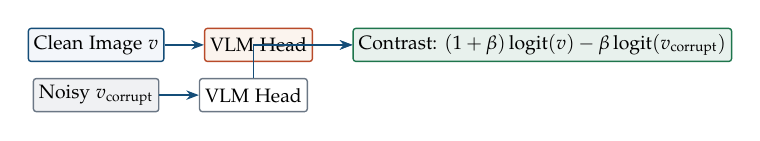
\begin{tikzpicture}[every node/.style={font=\scriptsize},node distance=2mm]
\node[box,draw=acc,fill=soft] (clean) {Clean Image $v$};
\node[box,draw=mute,fill=mute!10,below=2mm of clean] (noisy) {Noisy $v_{\text{corrupt}}$};
\node[box,draw=acc2,fill=soft2,right=5mm of clean] (vlm1) {VLM Head};
\node[box,draw=mute,right=5mm of noisy] (vlm2) {VLM Head};
\node[box,draw=acc3,fill=acc3!10,right=5mm of vlm1] (contrast) {Contrast: $(1+\beta)\operatorname{logit}(v) - \beta\operatorname{logit}(v_{\text{corrupt}})$};
\draw[arr] (clean)--(vlm1); \draw[arr] (noisy)--(vlm2);
\draw[arr] (vlm1)--(contrast); \draw[arr] (vlm2)|-(contrast);
\end{tikzpicture}%
}
\end{center}
\begin{itemize}
\item Creates a corrupted image $v_{\text{corrupt}}$ by adding Gaussian noise or blurring to destroy fine-grained visual details while keeping coarse text prompt $q$ identical.
\item Evaluates both original logits $p(y_t | v, q, y_{<t})$ and corrupted logits $p(y_t | v_{\text{corrupt}}, q, y_{<t})$.
\item Contrasts the two distributions at each decoding step:
$$\operatorname{logit}^*(y_t) = (1 + \beta) \operatorname{logit}(y_t | v) - \beta \operatorname{logit}(y_t | v_{\text{corrupt}}) \quad (\beta \approx 0.5-1.0)$$
\item Tokens driven purely by language priors have equal probability under both views and cancel out; tokens strongly grounded in visual evidence remain elevated.
\end{itemize}}
\end{qa}

\begin{qa}[High-Resolution Document Understanding \& MMMU]
\Q{What makes document understanding (DocVQA) fundamentally harder than natural image VLM tasks?}{
\begin{itemize}
\item \textbf{Aspect Ratio \& Scale}: Documents are typically tall portrait orientations ($8.5 \times 11$ inches, $>2000 \times 3000$ pixels). Resizing to square $336 \times 336$ or $448 \times 448$ shrinks 8pt fonts to sub-pixel noise, causing severe OCR failure.
\item \textbf{Reading Order \& Spatial Layout}: Text flows across multi-column tables, bounding boxes, and headers. Raster visual encoders lack explicit layout priors and scramble reading order without specialized 2D positional embeddings.
\item \textbf{Resolution Solution}: Modern models (Qwen2-VL, InternVL-2) use dynamic patch slicing (AnyRes) or native resolution processing, dividing high-res documents into $10-20$ localized sub-patches and preserving native $300$ DPI text fidelity.
\end{itemize}}

\Q{Why is MMMU considered the premier college-level evaluation for multimodal foundation models?}{
Unlike perception benchmarks testing whether a model sees a cat, MMMU evaluates expert reasoning across 30 college-level disciplines (Quantum Physics, Organic Chemistry, Structural Engineering, Medicine).
Questions involve multi-panel plots, circuit schematics, histological slides, and complex mathematical formulas, requiring joint perceptual parsing, spatial geometric projection, and multi-step domain reasoning.}
\end{qa}

\begin{trap}[VLM Evaluation Pitfalls]
\begin{itemize}
\item \textbf{Option Order Bias}: Multiple-choice benchmarks (e.g. MMBench) suffer from severe position bias (e.g., models prefer option "A" 60\% of the time). Always run \hl{circular evaluation} (evaluating all cyclic permutations A$\to$B$\to$C$\to$D and requiring correct answers on all permutations to grant a point).
\item \textbf{Data Contamination}: Many popular vision-language benchmarks (DocVQA, ScienceQA) have had their images scraped into web-scale pretraining datasets; always verify train-test split hashes.
\end{itemize}
\end{trap}

\section{Generative Diffusion: DDPM, DDIM \& Guidance}\label{sec:diff}
\lab{DDPM \textperiodcentered\ score SDE/ODE \textperiodcentered\ simplified loss \textperiodcentered\ DDIM ODE sampling \textperiodcentered\ EDM \textperiodcentered\ CFG}

\diagpair{%
\adjustbox{max width=\linewidth}{%
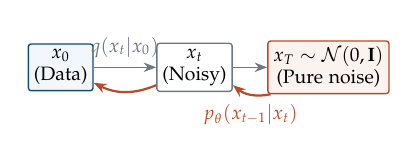
\begin{tikzpicture}[x=1mm,y=1mm,every node/.style={font=\scriptsize}]
\node[box,draw=acc,fill=soft] (x0) at (0,10) {$x_0$\\(Data)};
\node[box,draw=mute] (xt) at (17,10) {$x_t$\\(Noisy)};
\node[box,draw=acc2,fill=soft2] (xT) at (34,10) {$x_T \sim \mathcal{N}(0, \mathbf{I})$\\(Pure noise)};
\draw[arr,mute] (x0) -- (xt) node[midway,above] {$q(x_t|x_0)$};
\draw[arr,mute] (xt) -- (xT);
\draw[arr,acc2,thick] (xT) to[bend left=25] node[midway,below] {$p_\theta(x_{t-1}|x_t)$} (xt);
\draw[arr,acc2,thick] (xt) to[bend left=25] (x0);
\end{tikzpicture}%
}
}{%
\textbf{The Diffusion Duality.} Gradually corrupts data with Gaussian noise in the forward process; trains a neural network $\epsilon_\theta(x_t, t)$ to reverse the trajectory step-by-step.\\[2pt]
{\color{acc2}$\blacktriangleright$} \textbf{One-step noising}: Can jump directly to any timestep $t$ without simulating intermediate steps:
$x_t = \sqrt{\bar{\alpha}_t} x_0 + \sqrt{1 - \bar{\alpha}_t} \epsilon$, where $\epsilon \sim \mathcal{N}(0, \mathbf{I})$.
}

\begin{mem}[Mathematical Foundations of DDPM]
\begin{itemize}
\item \textbf{Noise schedule}: $\beta_1 < \dots < \beta_T$; $\alpha_t = 1 - \beta_t$; $\bar{\alpha}_t = \prod_{s=1}^t \alpha_s$.
\item \textbf{Training Objective ($\mathcal{L}_{\text{simple}}$)}: Predicts added noise $\epsilon$ via MSE:
$$\mathcal{L}_{\text{simple}}(\theta) = \mathbb{E}_{t \sim \mathcal{U}(1, T),\, x_0,\, \epsilon \sim \mathcal{N}(0, \mathbf{I})} \left[ \| \epsilon - \epsilon_\theta(x_t, t) \|^2 \right]$$
\item \textbf{Reverse Step}: Reconstructs $x_{t-1}$ from $x_t$:
$$x_{t-1} = \frac{1}{\sqrt{\alpha_t}} \left( x_t - \frac{\beta_t}{\sqrt{1 - \bar{\alpha}_t}} \epsilon_\theta(x_t, t) \right) + \sigma_t z \quad (z \sim \mathcal{N}(0, \mathbf{I}))$$
\end{itemize}
\end{mem}

\begin{center}
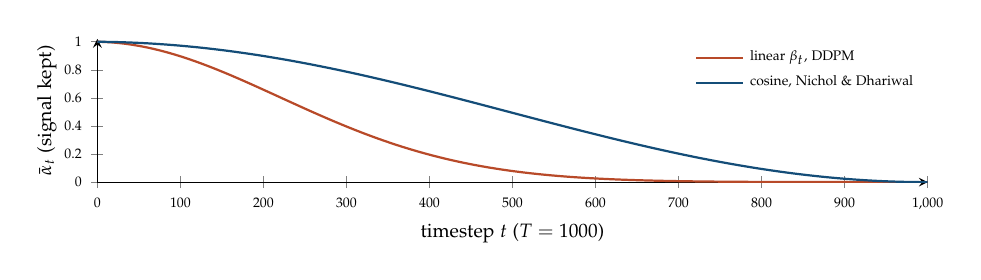
\begin{tikzpicture}
\begin{axis}[width=\columnwidth,height=34mm,xmin=0,xmax=1000,ymin=0,ymax=1.02,
  axis lines=left,xlabel={timestep $t$ ($T = 1000$)},ylabel={$\bar{\alpha}_t$ (signal kept)},
  tick label style={font=\tiny},label style={font=\scriptsize},
  xlabel style={yshift=2pt},ylabel style={yshift=-4pt},
  legend style={font=\tiny,draw=none,fill=none,at={(1,1)},anchor=north east},legend cell align=left,
  samples=120,domain=0:1000,every axis plot/.append style={line width=0.8pt}]
\addplot[acc2] {exp(-0.0001*x - 0.0199*x^2/2000)}; \addlegendentry{{linear $\beta_t$, DDPM}}
\addplot[acc] {cos(((x/1000+0.008)/1.008)*90)^2/cos((0.008/1.008)*90)^2}; \addlegendentry{{cosine, Nichol \& Dhariwal}}
\end{axis}
\end{tikzpicture}\\[-1pt]
{\scriptsize\color{mute}The linear schedule destroys almost all signal by $t \approx 600$, wasting the last 40\% of steps on near-pure noise; the cosine schedule degrades smoothly.}
\end{center}
\begin{qa}[Sampling Acceleration, SDE Theory \& Classifier-Free Guidance]
\Q{Derive the connection between DDPM and Continuous Score-Based SDEs.}{
Song et al. unify DDPM as the discretization of an Itô Stochastic Differential Equation:
\begin{itemize}
\item \textbf{Forward SDE}: $d\mathbf{x} = f(\mathbf{x}, t) dt + g(t) d\mathbf{w}$, where drift $f(\mathbf{x}, t) = -\frac{1}{2}\beta(t)\mathbf{x}$ and diffusion $g(t) = \sqrt{\beta(t)}$.
\item \textbf{Reverse-Time SDE}:
$$d\mathbf{x} = \left[ f(\mathbf{x}, t) - g(t)^2 \nabla_{\mathbf{x}} \log p_t(\mathbf{x}) \right] dt + g(t) d\mathbf{\bar{w}}$$
where $\nabla_{\mathbf{x}} \log p_t(\mathbf{x})$ is the \textbf{score function}. Tweedie's formula reveals that the score is directly proportional to predicted noise:
$$\nabla_{\mathbf{x}} \log p_t(\mathbf{x}) = -\frac{\epsilon_\theta(\mathbf{x}_t, t)}{\sqrt{1 - \bar{\alpha}_t}}$$
\item \textbf{Probability Flow ODE}: Removing the Brownian motion term $d\mathbf{\bar{w}}$ yields a deterministic ODE with identical marginal distributions:
$$d\mathbf{x} = \left[ f(\mathbf{x}, t) - \frac{1}{2} g(t)^2 \nabla_{\mathbf{x}} \log p_t(\mathbf{x}) \right] dt$$
Solvable using high-order numerical solvers (Runge-Kutta, DPM-Solver) in $15-20$ steps.
\end{itemize}}
\end{qa}

\begin{qa}[EDM Framework \& CFG Dynamics]
\Q{Why does EDM (Karras et al., 2022) replace discrete schedules with continuous noise $\sigma$?}{
Discrete $\beta$-schedules tie model weights to specific discrete step counts ($T=1000$).
\textbf{EDM Formulation}:
Parametrizes corruption continuously via noise standard deviation $\sigma$: $\mathbf{x} = \mathbf{y} + \mathbf{n}, \mathbf{n} \sim \mathcal{N}(0, \sigma^2 \mathbf{I})$.
Employs network preconditioning $D_\theta(\mathbf{x}; \sigma) = c_{\text{skip}}(\sigma) \mathbf{x} + c_{\text{out}}(\sigma) F_\theta(c_{\text{in}}(\sigma) \mathbf{x}; c_{\text{noise}}(\sigma))$ such that effective training loss variance remains constant across all noise levels:
$$\mathcal{L}_{\text{EDM}} = \mathbb{E}_{\mathbf{y}, \sigma, \mathbf{n}} \left[ \lambda(\sigma) \| D_\theta(\mathbf{y} + \mathbf{n}; \sigma) - \mathbf{y} \|_2^2 \right]$$
Samples $\ln(\sigma) \sim \mathcal{N}(P_{\text{mean}}, P_{\text{std}}^2)$, focusing model capacity on the mid-range noise levels that determine visual structure.}
\Q{How does Classifier-Free Guidance (CFG) work, and why does high guidance cause image burn?}{
\textbf{Mechanism}: In a text-to-image model, conditioning prompt $c$ is dropped with probability $p_{\text{uncond}} \approx 0.1-0.2$ during training (replaced with null embedding $\varnothing$).
At inference, both conditional and unconditional predictions are evaluated, and the score is extrapolated by guidance scale $s \ge 1.0$:
$$\tilde{\epsilon}_\theta(x_t, c) = \epsilon_\theta(x_t, \varnothing) + s \cdot \big(\epsilon_\theta(x_t, c) - \epsilon_\theta(x_t, \varnothing)\big)$$
\textbf{The trade-off}:
\begin{itemize}[leftmargin=*,itemsep=0.8pt]
\item $s = 1.0$: No guidance; samples follow true unconditional data distribution with high diversity but weak text alignment.
\item $s \in [5, 7.5]$: Optimal zone; sharpens semantics and adherence to prompt.
\item $s > 10$: Extrapolation forces latent values into extreme tails outside the training distribution, causing clipped latents, unnatural contrast, saturated colors, and "burn" artifacts.
\end{itemize}}
\end{qa}

\begin{trap}[Diffusion Numerical Traps]
\begin{itemize}
\item \textbf{Timestep Embedding}: Timestep $t$ must be mapped via sinusoidal positional embeddings followed by a 2-layer MLP before injection into ResNet/Attention blocks; feeding raw scalar integer $t$ prevents scale-invariant time conditioning.
\item \textbf{Variance Preserving vs Exploding}: DDPM uses Variance Preserving (VP) formulation ($\bar{\alpha}_t + (1-\bar{\alpha}_t) = 1$). EDM uses Variance Exploding (VE) where noise variance grows without bound: $x_t = x_0 + \sigma_t \epsilon$.
\end{itemize}
\end{trap}

\section{Latent Diffusion \& Diffusion Transformers (DiT)}\label{sec:ldm}
\lab{LDM \textperiodcentered\ Stable Diffusion \textperiodcentered\ VAE compression \textperiodcentered\ DiT \textperiodcentered\ adaLN-Zero \textperiodcentered\ SDXL}

\noindent\begin{minipage}[t]{0.42\columnwidth}\vspace{0pt}\centering
\resizebox{\linewidth}{!}{%
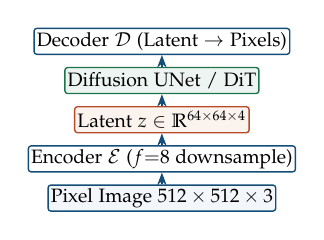
\begin{tikzpicture}[node distance=1.1mm,every node/.style={font=\tiny},
  bx/.style={box,minimum width=21mm,minimum height=3.3mm,inner sep=1pt}]
\node[bx,fill=soft] (img) {Pixel Image $512\times 512\times 3$};
\node[bx,draw=acc,above=1.5mm of img] (vae) {Encoder $\mathcal{E}$ ($f{=}8$ downsample)};
\node[bx,draw=acc2,fill=soft2,above=1.5mm of vae] (lat) {Latent $z \in \mathbb{R}^{64\times 64\times 4}$};
\node[bx,draw=acc3,fill=acc3!8,above=1.5mm of lat] (dit) {Diffusion UNet / DiT};
\node[bx,above=1.5mm of dit] (dec) {Decoder $\mathcal{D}$ (Latent $\to$ Pixels)};
\draw[arr] (img)--(vae); \draw[arr] (vae)--(lat); \draw[arr] (lat)--(dit); \draw[arr] (dit)--(dec);
\end{tikzpicture}%
}
\end{minipage}\hfill
\begin{minipage}[t]{0.56\columnwidth}\vspace{1pt}\small
\textbf{Perceptual vs Semantic Compression.} Pixel space diffusion wastes $>90\%$ of capacity on imperceptible high-frequency pixel noise.\\[2pt]
{\color{acc2}$\blacktriangleright$} \textbf{$f=8$ Compression}: $512\times 512\times 3 = 786{,}432$ values compressed to $64\times 64\times 4 = 16{,}384$ values ($48\times$ memory reduction).\\
{\color{acc2}$\blacktriangleright$} \textbf{Cross-modal injection}: Text conditioning injected into spatial latents via cross-attention.
\end{minipage}

\begin{mem}[Latent Diffusion Models Compared]
\begin{tabularx}{\linewidth}{@{}p{16mm} c p{22mm} X@{}}
\toprule
\textbf{Model} & \textbf{Params} & \textbf{Text Encoders} & \textbf{Conditioning / Backbone}\\
\midrule
\textbf{SD 1.5} & 860M & CLIP ViT-L/14 & UNet $512^2$, Cross-attention\\
\textbf{SD 2.1} & 865M & OpenCLIP-ViT-H & UNet $768^2$, $v$-pred, cross-attn\\
\textbf{SDXL}   & 2.6B & CLIP-L + OpenCLIP-G & UNet $1024^2$, Dual text, crop coords\\
\textbf{DiT-XL/2} & 675M & Class / CLIP tokens & Transformer $256^2$, adaLN-Zero\\
\bottomrule
\end{tabularx}
\end{mem}

\begin{qa}[Architecture Shifts: UNet to DiT]
\Q{Why did modern generative vision abandon convolutional UNets for Diffusion Transformers (DiT)?}{
\textbf{1. Scaling Laws}: Convolutional UNets plateau in generation quality as parameter counts scale past 2B due to fixed receptive fields and localized inductive biases. Transformers scale monotonically with compute and FLOPs without saturation.
\textbf{2. Flexible sequence handling}: UNets require rigid spatial grid tensors. DiT patchifies latents into 1D token sequences, making it trivial to process arbitrary aspect ratios, variable image resolutions, and temporal video frames in a single unified architecture.
\textbf{3. Hardware efficiency}: Standard dense matrix multiplications in Transformer self-attention achieve $>50\%$ MFU on Tensor Cores (especially with FlashAttention-2), whereas multi-scale UNet up/down convolutions suffer from high memory bandwidth overhead.}
\Q{How does adaLN-Zero work in DiT, and why is zero-initialization necessary?}{
Rather than injecting timestep and class embeddings via cross-attention, DiT uses \textbf{Adaptive Layer Normalization (adaLN)}:
A projection MLP maps the sum of timestep and condition embeddings $(t + c)$ into scale, shift, and gate parameters $(\gamma_1, \beta_1, \alpha_1, \gamma_2, \beta_2, \alpha_2)$:
\begin{align*}
h' &= h + \alpha_1 \cdot \text{Attention}\big((1 + \gamma_1)\odot \text{LN}(h) + \beta_1\big)\\
h_{\text{out}} &= h' + \alpha_2 \cdot \text{MLP}\big((1 + \gamma_2)\odot \text{LN}(h') + \beta_2\big)
\end{align*}
\textbf{Zero-Initialization}: The gating factors $\alpha_1, \alpha_2$ are initialized to \textbf{zero}.
At initialization, every DiT block acts as an exact identity function ($h_{\text{out}} = h$). Gradients flow cleanly through arbitrarily deep networks at step 0 without exploding or vanishing.}
\Q{How does SDXL eliminate training crop artifacts via micro-conditioning?}{
Previous diffusion models discarded non-square images by center-cropping them to $512\times 512$, teaching the model that subjects are often cut in half at image borders.
\textbf{SDXL Micro-Conditioning (Podell et al., 2023)}:
During training, random crops are drawn from variable aspect-ratio images, and the exact pixel crop coordinates $(c_{\text{top}}, c_{\text{left}})$ along with original resolution $(h_{\text{orig}}, w_{\text{orig}})$ are embedded via Fourier features and injected into the UNet conditioning vector.
At inference, setting $(c_{\text{top}}=0, c_{\text{left}}=0)$ conditions the model to generate fully uncropped, centered compositions.}
\end{qa}

\begin{trap}[Latent Diffusion Pitfalls]
\begin{itemize}
\item \textbf{VAE Latent Scaling Factor}: Latent representations from the VAE encoder have non-unit variance ($\sigma \ne 1$). SD scales latents by constant factor $0.18215$ (SDXL uses $0.13025$) before adding noise: $z = 0.18215 \cdot \mathcal{E}(x)$. Forgetting this scaling factor leads to complete generation failure (snow noise).
\item \textbf{Latent VAE artifacts}: High spatial compression ($f=8$) creates artifacts on fine typography and small faces. Face restorers (CodeFormer) or lower compression ($f=4$) are required for micro-detail reconstruction.
\end{itemize}
\end{trap}

\section{Flow Matching, Rectified Flow \& Flux.1}\label{sec:flow}
\lab{Flow Matching \textperiodcentered\ straight paths \textperiodcentered\ velocity objective \textperiodcentered\ Rectified Flow \textperiodcentered\ Flux.1 12B \textperiodcentered\ OT-CFM}

\diagpair{%
\adjustbox{max width=\linewidth}{%
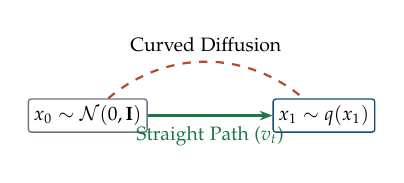
\begin{tikzpicture}[x=1mm,y=1mm,every node/.style={font=\scriptsize}]
\node[box,draw=mute] (x0) at (0,10) {$x_0 \sim \mathcal{N}(0, \mathbf{I})$};
\node[box,draw=acc] (x1) at (30,10) {$x_1 \sim q(x_1)$};
% Curved diffusion path
\draw[draw=acc2,thick,dashed] (x0) to[bend left=40] node[midway,above] {Curved Diffusion} (x1);
% Straight Flow Matching path
\draw[arr,acc3,very thick] (x0) -- (x1) node[midway,below] {Straight Path ($v_t$)};
\end{tikzpicture}%
}
}{%
\textbf{Straight Probability Paths.} Diffusion trajectories curve stochastically through latent space, requiring small steps.\\[2pt]
{\color{acc2}$\blacktriangleright$} \textbf{Constant Velocity Target}:
$x_t = (1 - t) x_0 + t x_1 \implies v_t = \frac{d x_t}{dt} = x_1 - x_0$\\[2pt]
{\color{acc2}$\blacktriangleright$} \textbf{Single-step Euler}: Straight paths make 1-to-4 step generation possible without distillation.
}

\begin{mem}[Flow Matching vs Diffusion Comparison]
\begin{tabularx}{\linewidth}{@{}p{18mm} X X@{}}
\toprule
\textbf{Property} & \textbf{Standard Diffusion (DDPM/EDM)} & \textbf{Flow Matching / Rectified Flow}\\
\midrule
\textbf{Trajectory} & Curved probability paths & \textbf{Straight} linear trajectories ($x_t = (1-t)x_0 + tx_1$)\\
\textbf{Prediction Target} & Noise $\epsilon_t$ or data $x_0$ & Constant velocity vector field $v_t = x_1 - x_0$\\
\textbf{Time Parameter} & Discrete $t \in [1, 1000]$ or continuous $\sigma$ & Normalized interval $t \in [0, 1]$\\
\textbf{Sampling Step} & Complex variance-adjusted ODE step & Simple linear update: $x_{t+\Delta t} = x_t + \Delta t \cdot v_\theta(x_t, t)$\\
\textbf{Few-Step Quality} & Blurry / degraded under 10 steps & Crisp, detailed generation in 4--8 steps\\
\bottomrule
\end{tabularx}
\end{mem}

\begin{qa}[Rectified Flow Mechanics \& Flux Architecture]
\Q{How does Rectified Flow straighten sampling paths, and what is Reflowing?}{
When training on random pairs of $(x_0, x_1)$ ($x_0$ random noise, $x_1$ data image), trajectories can cross each other in state space. Where paths cross, the vector field must predict the average velocity of diverging paths, inducing local curvature.
\textbf{Reflowing Procedure (2-Rectified Flow)}:
\begin{enumerate}[leftmargin=*,itemsep=0.8pt]
\item Generate synthetic pairs $(x_0, \hat{x}_1)$ by simulating the trained 1-rectified flow ODE from $t=0$ to $t=1$.
\item Train a new flow matching model on these deterministic coupled pairs $(x_0, \hat{x}_1)$.
\end{enumerate}
Because the pairs come from an ODE whose paths cannot cross (uniqueness of ODE solutions), the new coupling has less crossing and the learned paths are straighter; Liu et al.\ prove reflow never increases transport cost. In practice 2-rectified flow plus distillation gives good samples in \textbf{1 to 2 Euler steps}.}
\Q{What is Optimal Transport Flow Matching (OT-CFM)?}{
Tong et al.\ (2023) observe that standard flow matching pairs random Gaussian noise $x_0$ with random data $x_1$ independently, producing long, crossing trajectories.
\textbf{Optimal Transport CFM}: Couples pairs $(x_0, x_1)$ according to the optimal transport plan $\pi$ minimizing dynamic kinetic energy:
$$\mathcal{W}_2^2(p_0, p_1) = \inf_\pi \int \|x_0 - x_1\|_2^2 \, d\pi(x_0, x_1)$$
Solve exact OT (Hungarian / EMD) within each mini-batch and re-pair noise with data by that plan. Paths cross less, training variance drops and fewer ODE steps are needed; the benefit shrinks in high dimensions where mini-batch OT is a rough approximation.}
\Q{Walk through the 12B parameter architecture of Flux.1.}{
Flux.1 (Black Forest Labs) is an MM-DiT in the style of SD3, with no cross-attention:
\begin{enumerate}[leftmargin=*,itemsep=0.8pt]
\item \textbf{Double Stream Blocks (19 blocks)}: Image and text tokens keep \emph{separate weights} (norms, QKV, MLP) but run \emph{one joint attention} over the concatenated sequence, so each modality reads the other while keeping specialized parameters.
\item \textbf{Single Stream Blocks (38 blocks)}: Concatenates text and visual tokens into a single unified residual stream, running bidirectional self-attention across all tokens simultaneously.
\item \textbf{Dual Text Conditioning}: \textbf{T5-XXL} token sequence (prompt structure, spelling) enters the text stream; the pooled \textbf{CLIP ViT-L} vector is added to the timestep embedding for adaLN modulation (global style).
\item \textbf{Rotary Positional Embeddings (2D RoPE)}: Replaces fixed absolute coordinates, enabling training and inference across any aspect ratio and resolution up to 2.0 megapixels without tiling.
\end{enumerate}}
\end{qa}

\begin{trap}[Flow Matching Gotchas]
\begin{itemize}[leftmargin=*,itemsep=0.8pt]
\item \textbf{Direction of $t$}: In diffusion literature, $t=0$ is clean data and $t=T$ is pure noise. In Flow Matching literature, conventions are often \textbf{inverted}: $t=0$ is pure Gaussian noise ($x_0 \sim \mathcal{N}(0, \mathbf{I})$) and $t=1$ is target data ($x_1$). Check the boundary conditions of your solver ($0 \to 1$ vs $1 \to 0$).
\item \textbf{CFG formulation in Flow Matching}: Naive CFG extrapolation on velocity fields can overshoot data manifolds. Flux uses guidance distillation or interval-constrained CFG to prevent color explosion.
\end{itemize}
\end{trap}

\section{Video Foundation Models: Spatio-Temporal DiT}\label{sec:vid}
\lab{Factorized attention \textperiodcentered\ 3D VAE \textperiodcentered\ Space-Time DiT \textperiodcentered\ Sora mechanics \textperiodcentered\ Causal masking \textperiodcentered\ VBench}

\diagpair{%
\adjustbox{max width=\linewidth}{%
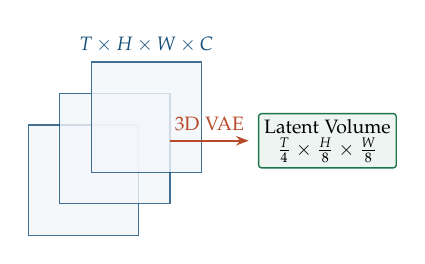
\begin{tikzpicture}[x=1mm,y=1mm,every node/.style={font=\scriptsize}]
\foreach \t in {0,4,8} {
  \draw[draw=acc,fill=soft,opacity=0.8] (\t,\t) rectangle (\t+14,\t+14);
}
\node[acc,above] at (15,22) {$T \times H \times W \times C$};
\draw[arr,acc2,thick] (18,12) -- (28,12) node[midway,above] {3D VAE};
\node[box,draw=acc3,fill=acc3!8] at (38,12) {Latent Volume\\$\frac{T}{4} \times \frac{H}{8} \times \frac{W}{8}$};
\end{tikzpicture}%
}
}{%
\textbf{The Spatio-Temporal Explosion.} Naive full 3D self-attention over video tensor $\mathbb{R}^{B \times C \times T \times H \times W}$ scales as $\mathcal{O}((T \cdot H \cdot W)^2)$, causing immediate out-of-memory crashes on GPU.\\[2pt]
{\color{acc2}$\blacktriangleright$} \textbf{Factorized Attention}: Decouples spatial attention (within frame) from temporal attention (across time) $\to \mathcal{O}(T(HW)^2 + (HW)T^2)$.
}

\begin{mem}[Video Representation Paradigms]
\begin{tabularx}{\linewidth}{@{}p{18mm} X X@{}}
\toprule
\textbf{Architecture} & \textbf{Mechanism} & \textbf{Trade-off}\\
\midrule
\textbf{3D Conv (I3D)} & Inflates $2\text{D } K^2 \to 3\text{D } K^3$; repeats weights divided by $K$ & Rigid temporal receptive field; high parameter overhead.\\
\textbf{Factorized ViT} (ViViT) & Alternates Spatial Self-Attn ($HW$ tokens) and Temporal ($T$ tokens) & Linear in $T$; enables training on $32-64$ frames on consumer clusters.\\
\textbf{3D DiT} (Sora) & Spatio-temporal 3D VAE ($8\times 8$ space, $4\times$ time) $+$ 3D DiT & Monotonic scaling; high fidelity; requires heavy compute clusters.\\
\bottomrule
\end{tabularx}
\end{mem}

\begin{qa}[Video Diffusion, 3D VAE \& Evaluation]
\Q{How does a 3D Spatio-Temporal VAE compress video, and why is temporal downsampling tricky?}{
A 10-second 1080p video at 24 FPS contains 240 frames $\approx 1.5\times 10^9$ raw values.
A \textbf{3D Causal VAE} compresses data along all 3 dimensions:
\begin{itemize}[leftmargin=*,itemsep=0.8pt]
\item Spatial: $8\times 8$ downsampling ($H/8, W/8$).
\item Temporal: $4\times$ downsampling ($T/4 \implies 60$ latent frames).
\end{itemize}
\textbf{The Challenge}: Pure 3D convolutions look into future frames, destroying causal streaming generation.
Modern video VAEs enforce \textbf{causal temporal convolutions} (padding only on past frames), ensuring that encoding/decoding frame $t$ never requires future frames $t+1$.}
\Q{How do modern video models (e.g. Sora, Movie Gen) achieve variable duration and aspect ratios?}{
Following the NaViT/Patch n' Pack paradigm:
\begin{enumerate}[leftmargin=*,itemsep=0.8pt]
\item \textbf{Spacetime Patches}: Video latents are partitioned into 3D spacetime cubes of size $p_t \times p_h \times p_w$ (e.g., $1 \times 2 \times 2$).
\item \textbf{Flattened Sequence}: Any video clip—regardless of resolution or duration—flattens into a 1D token sequence of length $N = \frac{T}{p_t} \cdot \frac{H}{p_h} \cdot \frac{W}{p_w}$.
\item \textbf{3D RoPE}: Position embeddings are decomposed into 3 rotary frequency components $(R_{\text{time}}, R_{\text{height}}, R_{\text{width}})$.
\end{enumerate}
Allows training on mixed datasets of vertical TikTok videos, widescreen 4K film clips, and images ($T=1$) in the same training batches without cropping or padding.}
\Q{Why is Fréchet Video Distance (FVD) flawed, and how does VBench fix it?}{
\textbf{Flaws of FVD}: FVD computes Fréchet distance on features from an I3D model pretrained on Kinetics-400. It is heavily biased toward low-resolution action recognition features, ignores temporal consistency (adjacent flickering frames can still produce identical average feature distributions), and penalizes stylistic artistic videos.
\textbf{VBench (Huang et al., 2024)}: Comprehensive evaluation decomposed into 16 distinct sub-benchmarks:
\begin{itemize}[leftmargin=*,itemsep=0.8pt]
\item \textbf{Temporal Quality}: Temporal flickering, motion smoothness, dynamic degree, subject consistency, background consistency.
\item \textbf{Video-Text Alignment}: Action accuracy, scene transitions, multiple objects, spatial relationships.
\end{itemize}
Evaluates using fine-tuned specialized vision models and tracking algorithms, providing granular diagnosis of video failure modes.}
\end{qa}

\begin{trap}[Video Generation Traps]
\begin{itemize}
\item \textbf{Flicker / Temporal Incoherence}: Training video diffusion without causal frame attention or 3D temporal discriminator losses causes adjacent frames to sample diverging textures ("boiling" noise artifacts).
\item \textbf{Autoregressive drift}: Extending video length by feeding the last generated frame as prompt for the next chunk suffers from error compounding; latents blur or explode after $10-15$ seconds without noise re-injection.
\end{itemize}
\end{trap}

\section{3D Vision: NeRF to 3D Gaussian Splatting}\label{sec:nerf}
\lab{NeRF \textperiodcentered\ Volume rendering \textperiodcentered\ Instant-NGP \textperiodcentered\ 3DGS covariance \textperiodcentered\ Tile rasterization \textperiodcentered\ SH radiance}

\noindent\begin{minipage}[t]{0.42\columnwidth}\vspace{0pt}\centering
\resizebox{\linewidth}{!}{%
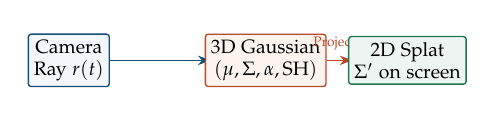
\begin{tikzpicture}[x=1mm,y=1mm,every node/.style={font=\tiny}]
\node[box,draw=acc,fill=soft] (cam) at (0,10) {Camera\\Ray $r(t)$};
\draw[arr,acc] (cam) -- (18,10);
\node[box,draw=acc2,fill=soft2] (g) at (25,10) {3D Gaussian\\$(\mu, \Sigma, \alpha, \text{SH})$};
\draw[arr,acc2] (g) -- (36,10) node[midway,above] {Project $J$};
\node[box,draw=acc3,fill=acc3!8] (px) at (43,10) {2D Splat\\$\Sigma'$ on screen};
\end{tikzpicture}%
}
\end{minipage}\hfill
\begin{minipage}[t]{0.56\columnwidth}\vspace{1pt}\small
\textbf{Implicit vs Explicit 3D.} NeRF represents scenes implicitly via continuous MLPs. 3D Gaussian Splatting (3DGS) represents scenes explicitly via millions of anisotropic 3D Gaussians.\\[2pt]
{\color{acc2}$\blacktriangleright$} \textbf{3DGS Real-Time Rendering}: Replaces expensive volumetric MLP ray-marching with GPU tile-based rasterization at $>100\text{ FPS}$.
\end{minipage}

\begin{mem}[Parameters per 3D Gaussian (Total: 59 floats $\approx 236$ bytes)]
\begin{tabularx}{\linewidth}{@{}p{18mm} c X@{}}
\toprule
\textbf{Property} & \textbf{Floats} & \textbf{Mathematical Representation}\\
\midrule
Position ($\mu$) & 3 & 3D world center $[x, y, z]^\top \in \mathbb{R}^3$\\
Scale ($s$) & 3 & Diagonal scaling vector $S = \text{diag}(s_x, s_y, s_z)$\\
Rotation ($q$) & 4 & Unit quaternion representing rotation $R \in SO(3)$\\
Opacity ($\alpha$) & 1 & Density parameter $\alpha \in [0, 1]$ passed through sigmoid\\
Color (SH) & 48 & Degree-3 Spherical Harmonics ($16\text{ coeffs} \times 3\text{ RGB}$)\\
\bottomrule
\end{tabularx}
\end{mem}

\begin{qa}[3D Representation, NeRF \& Gaussian Rasterization]
\Q{Walk through the Volume Rendering equation in NeRF and its discrete quadrature.}{
NeRF casts a ray $r(t) = \mathbf{o} + t \mathbf{d}$ from camera origin $\mathbf{o}$ along direction $\mathbf{d}$.
The continuous color integral between near and far bounds $[t_n, t_f]$ is:
$$C(r) = \int_{t_n}^{t_f} T(t) \cdot \sigma(r(t)) \cdot c(r(t), \mathbf{d})\, dt$$
$$\text{where } T(t) = \exp\left(-\int_{t_n}^t \sigma(r(s))\, ds\right)$$
$T(t)$ is \textbf{transmittance} (probability the ray traverses from $t_n$ to $t$ without hitting particles).
\textbf{Discrete Numerical Quadrature}: Sample $N$ points along the ray:
$$C(r) \approx \sum_{i=1}^N T_i \cdot \alpha_i \cdot c_i \quad \text{with } \alpha_i = 1 - \exp(-\sigma_i \delta_i), \quad T_i = \prod_{j=1}^{i-1} (1 - \alpha_j)$$
Evaluating this on a $1080\text{p}$ image requires $\approx 200\text{M}$ MLP forward passes, bounding vanilla NeRF to several seconds per frame.}
\Q{How does Instant-NGP accelerate NeRF training from days to seconds?}{
Müller et al. identify that large MLPs are slow to evaluate and suffer from spectral bias on high spatial frequencies.
\textbf{Instant-NGP (Multiresolution Hash Encoding)}:
\begin{enumerate}[leftmargin=*,itemsep=0.8pt]
\item Discretizes 3D space into $L=16$ hierarchical grid levels with geometric progression of resolutions $N_l$.
\item Maps voxel corners to a fixed-size hash table of size $T=2^{19}$ using spatial hashing: $h(\mathbf{x}) = \left(\bigoplus_{i=1}^3 x_i \pi_i\right) \pmod T$.
\item Interpolates feature vectors ($d=2$ per level) trilinearly within the voxel.
\item Feeds concatenated features ($16 \times 2 = 32$-dim) into a tiny 2-layer MLP (64 neurons) implemented with fully fused CUDA kernels.
\end{enumerate}
Trains high-quality radiance fields in \textbf{5 seconds}.}
\Q{How does 3D Gaussian Splatting project 3D ellipsoids onto a 2D screen?}{
A 3D Gaussian has spatial density $G(x) = \exp\left(-\frac{1}{2}(x - \mu)^\top \Sigma^{-1} (x - \mu)\right)$.
Its 3D covariance is parameterized as $\Sigma = R S S^\top R^\top$.
To project onto the 2D image plane, Zwicker et al. apply an affine approximation via viewing transformation matrix $W$ and projective Jacobian $J$:
$$\Sigma' = \mathbf{J} \mathbf{W} \mathbf{\Sigma} \mathbf{W}^\top \mathbf{J}^\top$$
$\Sigma'$ is a $2\times 2$ positive semi-definite screen-space covariance matrix.
The GPU rasterizer divides the screen into $16\times 16$ pixel tiles, sorts overlapping Gaussians by depth via fast radix sort, and accumulates color via front-to-back $\alpha$-blending without casting rays.}
\end{qa}

\begin{trap}[3D Vision Pitfalls]
\begin{itemize}[leftmargin=*,itemsep=0.8pt]
\item \textbf{Needle and Floater Artifacts in 3DGS}: Excessively large Gaussians in under-constrained background regions create needle-like spikes. Periodic \textbf{opacity reset} (forcing all $\alpha \to 0$ every $3000$ steps) prunes spurious floaters.
\item \textbf{Camera coordinate conventions}: OpenCV uses $(X \text{ right}, Y \text{ down}, Z \text{ forward})$; OpenGL/Blender uses $(X \text{ right}, Y \text{ up}, Z \text{ backward})$. Mixing coordinate conventions flips camera rays and produces completely black renders.
\end{itemize}
\end{trap}

\section{3D Gaussian Splatting: Math, Rasterizer \& SH}\label{sec:3dgs-deep}
\lab{3D Covariance $\Sigma$ \textperiodcentered\ EWA Jacobian projection \textperiodcentered\ Spherical Harmonics \textperiodcentered\ 64-bit Radix Sort \textperiodcentered\ Adaptive density control}

\begin{mem}[Parameters per 3D Gaussian Primitive]
\begin{tabularx}{\columnwidth}{@{}p{18mm} p{12mm} p{9mm} X@{}}
\toprule
\textbf{Attribute} & \textbf{Shape} & \textbf{Type} & \textbf{Mathematical Representation / Activation} \\
\midrule
\textbf{Position ($\mu$)} & 3 floats & $\mathbb{R}^3$ & World coordinates $(x, y, z)$ \\
\textbf{Scale ($s$)} & 3 floats & $\mathbb{R}^3$ & Semi-axis lengths via exponential $\exp(s) > 0$ \\
\textbf{Rotation ($q$)} & 4 floats & $\mathbb{H}$ & Unit quaternion $(w, x, y, z) / \|q\|$ \\
\textbf{Opacity ($\alpha$)} & 1 float & $[0, 1]$ & Blending density via sigmoid $\sigma(\alpha)$ \\
\textbf{Color / SH} & 48 floats & $\mathbb{R}^{3 \times 16}$ & Spherical Harmonics degree 3 ($16 \times 3$ RGB) \\
\midrule
\multicolumn{4}{@{}X@{}}{\textbf{Total Memory Footprint}: $59\text{ floats} \times 4\text{ bytes} \approx \mathbf{236\text{ bytes per Gaussian}}$. At $3\text{M Gaussians} \implies \mathbf{\sim 708\text{ MB}}$.} \\
\bottomrule
\end{tabularx}
\end{mem}

\begin{qa}[3D Covariance Parameterization \& EWA Projection]
\Q{Derive why 3DGS parameterizes covariance as $\Sigma = R S S^T R^T$ and how it projects into 2D screen space.}{
A valid covariance matrix must be \hl{symmetric positive semi-definite} ($\Sigma \succeq 0$).
Directly optimizing $\Sigma \in \mathbb{R}^{3 \times 3}$ violates positive definiteness during gradient descent, causing imaginary eigenvalues and catastrophic collapse.\\[2pt]
\textbf{Decomposition into Scale and Rotation}:
\begin{itemize}
\item $\mathbf{S} = \operatorname{diag}(\exp(s_x), \exp(s_y), \exp(s_z))$ guarantees non-zero real scaling.
\item $\mathbf{R} \in \operatorname{SO}(3)$ is computed from normalized unit quaternion $\mathbf{q} = (w, x, y, z) / \sqrt{w^2+x^2+y^2+z^2}$.
\item Thus $\mathbf{\Sigma} = \mathbf{R} \mathbf{S} \mathbf{S}^T \mathbf{R}^T$ is mathematically guaranteed to be symmetric positive semi-definite.
\end{itemize}
\textbf{2D EWA Projection (Zwicker et al.)}:
Given camera viewing transformation $\mathbf{W}$ (world-to-camera matrix) and projective transformation, the 2D projected covariance $\mathbf{\Sigma}' \in \mathbb{R}^{2 \times 2}$ is given by:
$$\mathbf{\Sigma}' = \mathbf{J} \mathbf{W} \mathbf{\Sigma} \mathbf{W}^T \mathbf{J}^T + 0.3 \cdot \mathbf{I}_{2 \times 2}$$
where $\mathbf{J}$ is the Jacobian of the affine approximation of projective transformation evaluated at camera coordinates $(t_x, t_y, t_z)$:
$$\mathbf{J} = \begin{bmatrix} \frac{f_x}{t_z} & 0 & -\frac{f_x t_x}{t_z^2} \\ 0 & \frac{f_y}{t_z} & -\frac{f_y t_y}{t_z^2} \end{bmatrix}$$
The term $0.3 \cdot \mathbf{I}_{2 \times 2}$ acts as a low-pass Gaussian blur filter, preventing aliasing artifacts when a splat projects to an area smaller than a single pixel.}

\Q{Explain how Spherical Harmonics model view-dependent specular reflections in 3DGS.}{
Lambertian surfaces reflect light uniformly in all directions; non-Lambertian surfaces (metals, mirrors, glass) reflect different colors depending on viewing direction $\mathbf{d} = \frac{\mathbf{x} - \mathbf{c}}{\|\mathbf{x} - \mathbf{c}\|}$.\\[2pt]
\textbf{Spherical Harmonics (SH) Expansion}:
Color $c(\mathbf{d}) \in \mathbb{R}^3$ is modeled as a linear combination of orthonormal basis functions $Y_l^m(\mathbf{d})$ on the unit sphere:
$$c(\mathbf{d}) = \sum_{l=0}^{l_{\max}} \sum_{m=-l}^l k_l^m \, Y_l^m(\mathbf{d})$$
\begin{itemize}
\item \textbf{Degree 0 ($l=0, 1$ basis)}: $Y_0^0 = \frac{1}{2}\sqrt{\frac{1}{\pi}}$. Represents constant ambient/diffuse color (1 coeff $\times 3 = 3$ floats).
\item \textbf{Degree 1 ($l=1, 3$ bases)}: Directional gradient (4 total coeffs $\times 3 = 12$ floats).
\item \textbf{Degree 2 ($l=2, 5$ bases)}: Quadric reflection lobes (9 total coeffs $\times 3 = 27$ floats).
\item \textbf{Degree 3 ($l=3, 7$ bases)}: Sharp specular highlights (16 total coeffs $\times 3 = 48$ floats).
\end{itemize}}
\end{qa}

\begin{qa}[Tile-Based Tile Rasterizer \& Adaptive Densification]
\Q{Step through the GPU tile-based rasterization pipeline that enables 100+ FPS real-time rendering.}{
\begin{enumerate}
\item \textbf{Screen Tiling}: Divides display resolution into non-overlapping $16 \times 16$ pixel tiles.
\item \textbf{Culling \& Bounding}: Evaluates $99\%$ confidence ellipse ($3\sigma$) for each 2D projected Gaussian $\mathbf{\Sigma}'$; discards splats outside viewing frustum.
\item \textbf{Tile Assignment \& 64-bit Key}: For each tile a Gaussian overlaps, generates a duplicate 64-bit integer key:
$$\text{Key} = [\text{Tile ID (32-bit)} \mid \text{Viewspace Depth } z \text{ (32-bit)}]$$
\item \textbf{GPU Radix Sort}: A single parallel GPU Radix Sort orders all key-value pairs by Tile ID, and within each tile, strictly front-to-back by depth $z$.
\item \textbf{Tile Rasterization Warp}: One thread block processes one tile; threads load sorted Gaussians into shared memory and blend colors front-to-back:
$$C_{\text{pixel}} = \sum_{i=1}^N c_i \alpha_i \prod_{j=1}^{i-1} (1 - \alpha_j), \quad \alpha_i = \sigma_i \exp\left(-\frac{1}{2} \Delta^T {\mathbf{\Sigma}'}^{-1} \Delta\right)$$
\item \textbf{Early Ray Termination}: Accumulates transmittance $T_i = \prod_{j=1}^{i-1}(1 - \alpha_j)$; once $T_i < 0.0001$, rendering terminates immediately for that pixel.
\end{enumerate}}

\Q{How does Adaptive Density Control decide whether to Clone or Split a 3D Gaussian?}{
During optimization, 3DGS tracks the average viewspace position gradient magnitude $\nabla_p = \|\frac{\partial \mathcal{L}}{\partial \mu_{2D}}\|_2$.
If $\nabla_p > \tau_{\text{pos}} = 0.0002$, the region is improperly reconstructed:
\begin{itemize}
\item \textbf{If Scale is Small ($\max(s) < \tau_{\text{scale}}$)}: Represents an \hl{under-reconstructed} region (e.g. missing thin bicycle spokes or leaf geometry). The Gaussian is \textbf{cloned} (duplicated) and shifted along the gradient direction.
\item \textbf{If Scale is Large ($\max(s) > \tau_{\text{scale}}$)}: Represents an \hl{over-reconstructed} region (a huge Gaussian trying to cover too much space). The Gaussian is \textbf{split} into two smaller Gaussians, each scaled down by factor $1.6\times$.
\item \textbf{Opacity Reset \& Pruning}: Every $3000$ iterations, opacities are reset to near-zero ($\alpha \leftarrow \min(\alpha, 0.01)$); Gaussians unable to rebuild opacity ($\alpha < 0.005$) are permanently pruned.
\end{itemize}}
\end{qa}

\begin{trap}[3DGS Optimization Pitfalls]
\begin{itemize}
\item \textbf{Needle Floater Artifacts}: Large background Gaussians very close to the camera form huge translucent "needle" streaks when rotated. Solution: Clamp minimum depth $z_{\text{near}}$ and penalize maximum spatial scale $\|s\|_\infty$ in the loss.
\item \textbf{Memory Thrashing during Densification}: Without periodic opacity pruning ($\alpha < 0.005$), Gaussian count explodes from $1\text{M} \to 12\text{M}$, exhausting GPU VRAM during training.
\end{itemize}
\end{trap}

\section{Vision Benchmarks, Metrics \& Evaluation}\label{sec:eval}
\lab{ImageNet-C \textperiodcentered\ COCO mAP \textperiodcentered\ Panoptic PQ \textperiodcentered\ FID 50k \textperiodcentered\ PSNR / SSIM / LPIPS}

\diagpair{%
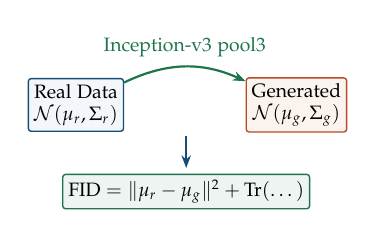
\begin{tikzpicture}[x=1mm,y=1mm,every node/.style={font=\scriptsize}]
\node[box,draw=acc,fill=soft] (r) at (0,10) {Real Data\\$\mathcal{N}(\mu_r, \Sigma_r)$};
\node[box,draw=acc2,fill=soft2] (g) at (28,10) {Generated\\$\mathcal{N}(\mu_g, \Sigma_g)$};
\draw[arr,acc3,thick] (r) to[bend left=25] node[midway,above] {Inception-v3 pool3} (g);
\node[box,draw=acc3,fill=acc3!8] at (14,-1) {$\text{FID} = \|\mu_r - \mu_g\|^2 + \text{Tr}(\dots)$};
\draw[arr] (14,6) -- (14,2);
\end{tikzpicture}
}{%
\textbf{The Evaluation Landscape.} Visual evaluation spans categorical recognition, dense pixel geometry, perceptual fidelity, and multimodal reasoning.\\[2pt]
{\color{acc2}$\blacktriangleright$} \textbf{COCO $\text{mAP}$}: Evaluated across 10 IoU thresholds from $0.50$ to $0.95$ with $0.05$ step size.\\
{\color{acc2}$\blacktriangleright$} \textbf{FID}: Measures 2-Wasserstein distance between multivariate Gaussian features in Inception space.
}

\begin{mem}[Key Vision Benchmarks \& Thresholds]
\begin{tabularx}{\linewidth}{@{}lLL@{}}
\toprule
\textbf{Domain} & \textbf{Benchmark} & \textbf{Standard Metric}\\
\midrule
\textbf{Classification} & ImageNet-1K, ImageNet-A/R/C & Top-1 Acc ($\%$) / Mean Corruption Error (mCE)\\
\textbf{Detection} & MS COCO (80 classes) & $\text{mAP}_{50:95}$, $\text{AP}_{S}$, $\text{AP}_{M}$, $\text{AP}_{L}$\\
\textbf{Segmentation} & ADE20K (semantic), Cityscapes & Mean IoU (mIoU), Panoptic Quality ($\text{PQ} = \text{SQ} \times \text{RQ}$)\\
\textbf{VLM Reasoning} & MMBench, MathVista, DocVQA & Overall Accuracy, OCR-F1 score\\
\textbf{Hallucination} & POPE (Random, Popular, Adversarial) & Binary F1-score \& Yes-ratio\\
\textbf{Generative} & ImageNet $512^2$, COCO 30k & $\text{FID}$ ($<3.0$ frontier), CLIP Score ($>30.0$)\\
\textbf{3D Quality} & NeRF Synthetic, Tanks \& Temples & PSNR ($>32\text{ dB}$), SSIM ($>0.95$), LPIPS ($<0.05$)\\
\bottomrule
\end{tabularx}
\end{mem}

\begin{qa}[Metric Formulations \& Evaluator Pitfalls]
\Q{State the Fréchet Inception Distance (FID) formula and explain its vulnerabilities.}{
Given feature representations from the 2048-dimensional pool3 layer of Inception-v3:
$$\text{FID} = \|\mu_r - \mu_g\|_2^2 + \text{Tr}\left(\mathbf{\Sigma}_r + \mathbf{\Sigma}_g - 2(\mathbf{\Sigma}_r \mathbf{\Sigma}_g)^{1/2}\right)$$
This is the 2-Wasserstein distance between two continuous Gaussians $\mathcal{N}(\mu_r, \Sigma_r)$ and $\mathcal{N}(\mu_g, \Sigma_g)$.
\textbf{Vulnerabilities}:
\begin{enumerate}[leftmargin=*,itemsep=0.8pt]
\item \textbf{Sample Size Sensitivity}: FID is biased upward with small sample counts; comparing FID requires evaluating on exactly 50,000 generated samples ($N=50\text{k}$).
\item \textbf{Inception Bias}: Inception-v3 was trained on ImageNet and is blind to human anatomy, facial distortion, text spelling, and high-frequency noise.
\item \textbf{JPEG and Resizing artifacts}: Compressing images or using bilinear rather than bicubic resizing alters FID by up to $\pm 5$ points without perceptible image differences.
\end{enumerate}}
\Q{PSNR vs SSIM vs LPIPS: what does each measure, and when does each lie?}{
\textbf{PSNR} $= 10 \log_{10}\frac{\text{MAX}^2}{\text{MSE}}$ dB. Pixel-wise; a 1-pixel shift or slight blur can cost several dB while looking identical, and blurry averages score well. $+1$ dB $\approx$ 21\% lower MSE.\\
\textbf{SSIM} compares local means, variances and covariance (luminance, contrast, structure) in $11\times 11$ Gaussian windows:
$$\text{SSIM} = \frac{(2\mu_x\mu_y + C_1)(2\sigma_{xy} + C_2)}{(\mu_x^2 + \mu_y^2 + C_1)(\sigma_x^2 + \sigma_y^2 + C_2)}$$
Better on structure, still insensitive to texture realism.\\
\textbf{LPIPS}: distance between unit-normalized deep features (AlexNet/VGG) with learned per-channel weights, trained on human 2AFC judgements. Tracks perceived similarity best; lower is better.\\
\textbf{Rule}: report all three for reconstruction (NeRF/3DGS, super-resolution, VAE); a GAN-sharpened output can lose PSNR but win LPIPS. For generation without a reference image, use FID/CLIPScore instead.}
\Q{How is Panoptic Quality (PQ) decomposed into SQ and RQ?}{
Kirillov et al. decompose Panoptic Quality as $\text{PQ} = \text{SQ} \times \text{RQ}$:
$$\text{SQ} = \frac{\sum_{(p, g) \in TP} \text{IoU}(p, g)}{|TP|}, \quad \text{RQ} = \frac{|TP|}{|TP| + \frac{1}{2}|FP| + \frac{1}{2}|FN|}$$
\begin{itemize}[leftmargin=*,itemsep=0.8pt]
\item \textbf{Segmentation Quality (SQ)}: Measures average boundary overlap purely among true-positive matched segments ($\text{IoU} > 0.5$).
\item \textbf{Recognition Quality (RQ)}: Standard F1-score measuring detection/classification accuracy of segments regardless of pixel tightness.
\end{itemize}
Decouples mask boundary quality from false-positive detection errors.}
\end{qa}

\begin{trap}[Benchmarking Traps]
\begin{itemize}
\item \textbf{ImageNet-C Corruption Leakage}: Using Gaussian blur or noise during training data augmentation contaminates ImageNet-C evaluation, invalidating reported robustness metrics.
\item \textbf{CLIPScore Gamification}: Generating images with giant repeated text labels exploits CLIP's text-matching bias, yielding high CLIPScore despite awful visual image quality.
\end{itemize}
\end{trap}

\section{Production Vision, Optimization \& Edge Deployment}\label{sec:prod}
\lab{Preprocessing \textperiodcentered\ Conv-BN fusion \textperiodcentered\ TensorRT \textperiodcentered\ INT8 PTQ \textperiodcentered\ Edge latency budgets \textperiodcentered\ ByteTrack}

\noindent\begin{minipage}[t]{0.42\columnwidth}\vspace{0pt}\centering
\resizebox{\linewidth}{!}{%
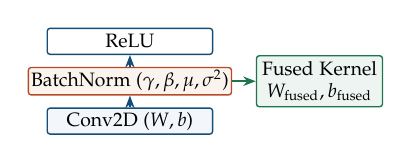
\begin{tikzpicture}[node distance=1.1mm,every node/.style={font=\tiny},
  bx/.style={box,minimum width=21mm,minimum height=3.3mm,inner sep=1pt}]
\node[bx,fill=soft] (c) {Conv2D ($W, b$)};
\node[bx,draw=acc2,fill=soft2,above=1.5mm of c] (bn) {BatchNorm ($\gamma, \beta, \mu, \sigma^2$)};
\node[bx,above=1.5mm of bn] (r) {ReLU};
\draw[arr] (c)--(bn); \draw[arr] (bn)--(r);
\node[box,draw=acc3,fill=acc3!8,right=3mm of bn] (f) {Fused Kernel\\$W_{\text{fused}}, b_{\text{fused}}$};
\draw[arr,acc3,thick] (bn.east) -- (f.west);
\end{tikzpicture}%
}
\end{minipage}\hfill
\begin{minipage}[t]{0.56\columnwidth}\vspace{1pt}\small
\textbf{The Zero-Cost Fusion.} BatchNorm parameters are linear and static at test time.\\[2pt]
{\color{acc2}$\blacktriangleright$} \textbf{Folding into Weights}:
$W_{\text{fused}} = \frac{\gamma}{\sqrt{\sigma^2+\epsilon}} W,\quad b_{\text{fused}} = \frac{\gamma}{\sqrt{\sigma^2+\epsilon}}(b-\mu) + \beta$\\[2pt]
{\color{acc2}$\blacktriangleright$} Eliminates $2\times$ memory roundtrips to GPU DRAM per convolution block.
\end{minipage}

\begin{mem}[Edge Inference Latency Budgets (Target: Real-Time)]
\begin{tabularx}{\linewidth}{@{}p{22mm} c X@{}}
\toprule
\textbf{Application} & \textbf{Budget} & \textbf{Recommended Model Architecture}\\
\midrule
\textbf{Robotics / Drones} & $16.6\text{ ms}$ & YOLOv8-Nano / MobileNetV4 / TensorRT INT8\\
\textbf{Auto Driving} & $33.3\text{ ms}$ & RegNet / ConvNeXt-T / BEVDet on NVIDIA Orin\\
\textbf{AR / VR} & $11.1\text{ ms}$ & 3D Gaussian Splatting with Metal/Vulkan\\
\textbf{Mobile Phone} & $33.3\text{ ms}$ & Apple CoreML Neural Engine / INT8 VLM\\
\bottomrule
\end{tabularx}
\end{mem}

\begin{qa}[Production Pipeline Dynamics \& Optimizations]
\Q{Derive the exact mathematical equations for fusing Conv2D and BatchNorm.}{
A Conv2D layer computes $x_{\text{conv}} = W x + b$.
BatchNorm normalizes and scales: $y = \gamma \frac{x_{\text{conv}} - \mu}{\sqrt{\sigma^2 + \epsilon}} + \beta$.
Substituting $x_{\text{conv}}$ directly into the BatchNorm formula:
\begin{align*}
y &= \gamma \frac{(W x + b) - \mu}{\sqrt{\sigma^2 + \epsilon}} + \beta\\
&= \left( \frac{\gamma}{\sqrt{\sigma^2 + \epsilon}} W \right) x + \left( \frac{\gamma}{\sqrt{\sigma^2 + \epsilon}} (b - \mu) + \beta \right)
\end{align*}
Define fused weights and bias:
\begin{align*}
W_{\text{fused}} &= \frac{\gamma}{\sqrt{\sigma^2 + \epsilon}} W\\
b_{\text{fused}} &= \frac{\gamma}{\sqrt{\sigma^2 + \epsilon}} (b - \mu) + \beta
\end{align*}
$W_{\text{fused}}$ is a standard $C_{\text{out}} \times C_{\text{in}} \times K \times K$ tensor and $b_{\text{fused}}$ is a $C_{\text{out}}$ vector. The BatchNorm operation and its memory allocation are completely eliminated at test time.}
\Q{Why does BGR vs RGB channel order cause a 30-point accuracy drop, and how is it audited?}{
OpenCV reads image buffers from disk or webcam in \textbf{BGR} format by default. PyTorch and Torchvision backbones (ResNet, ViT, CLIP) are trained exclusively on \textbf{RGB} arrays.
Feeding BGR images into an RGB-trained model swaps the red and blue channels:
skin tones become bright cyan/blue; blue skies become reddish-orange.
\textbf{Auditing Rule}: Always assert channel ordering at pipeline entry:
\lstinline|img = cv2.cvtColor(bgr_frame, cv2.COLOR_BGR2RGB)|.
Add a static unit test asserting that average red channel intensity of an Apple image exceeds blue intensity.}
\Q{Walk through INT8 Post-Training Quantization (PTQ) with KL Calibration.}{
FP32 weights and activations are mapped to 8-bit integers $[-128, 127]$ via scaling factor $S$: $x_{\text{int8}} = \text{clip}\left(\text{round}(x / S), -128, 127\right)$.
For activations with long-tail outlier distributions, clipping at the maximum absolute value wastes precision on rare extremes.
\textbf{NVIDIA TensorRT KL Calibration}:
\begin{enumerate}[leftmargin=*,itemsep=0.8pt]
\item Collect activation histograms over a calibration dataset ($\sim 500$ representative images).
\item For candidate clipping thresholds $T$: compute quantized and reconstructed distribution $P$ and $Q$.
\item Choose threshold $T^*$ minimizing Kullback-Leibler divergence:
$$T^* = \arg\min_T D_{\text{KL}}(P \parallel Q) = \sum_{i} P(i) \log \frac{P(i)}{Q(i)}$$
\end{enumerate}
Retains $99.5\%$ of FP32 accuracy while cutting memory bandwidth by $4\times$ and doubling compute throughput on Tensor Cores.}
\Q{How does ByteTrack track multi-object targets across occlusions in real time?}{
Traditional tracking-by-detection algorithms (SORT, DeepSORT) discard low-confidence detections ($s < 0.6$), losing targets during occlusions.
\textbf{ByteTrack (Zhang et al., 2022)}:
\begin{enumerate}[leftmargin=*,itemsep=0.8pt]
\item First Association: Matches high-score detections ($s \ge 0.6$) with existing tracklets using Kalman filter motion predictions and bounding box IoU.
\item Second Association: Takes the unmatched tracklets and matches them with \textbf{low-score detections} ($0.1 \le s < 0.6$).
\end{enumerate}
Low-confidence detections typically represent partially occluded or blurred objects. Re-associating them preserves target identity across obstacles at $>60\text{ FPS}$ with zero neural network re-evaluation.}
\end{qa}

\begin{trap}[Deployment Traps]
\begin{itemize}
\item \textbf{Letterboxing vs Stretching}: Resizing non-square camera feeds ($1920\times 1080$) to $640\times 640$ via simple stretching warps aspect ratios, corrupting bounding box regression and object detection confidence. Letterbox with symmetric grey borders (\texttt{114, 114, 114}).
\item \textbf{Synchronous video loops}: Calling \lstinline|cap.read()| synchronously inside the inference loop blocks GPU execution waiting for camera USB/MIPI driver I/O. Use a double-buffered background thread for frame acquisition.
\end{itemize}
\end{trap}

\section{Vision System Design: Autonomous Driving to Visual RAG}\label{sec:sys}
\lab{System design framework \textperiodcentered\ BEV driving perception \textperiodcentered\ Visual Document RAG \textperiodcentered\ Sub-second GenAI API \textperiodcentered\ ColPali}

\diagpair{%
\adjustbox{max width=\linewidth}{%
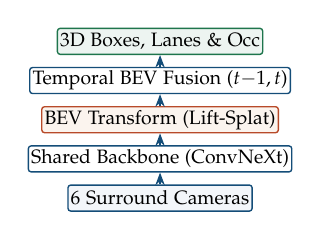
\begin{tikzpicture}[node distance=1.1mm,every node/.style={font=\scriptsize},
  bx/.style={box,minimum width=21mm,minimum height=3.3mm,inner sep=1pt}]
\node[bx,fill=soft] (cam) {6 Surround Cameras};
\node[bx,draw=acc,above=1.5mm of cam] (bb) {Shared Backbone (ConvNeXt)};
\node[bx,draw=acc2,fill=soft2,above=1.5mm of bb] (bev) {BEV Transform (Lift-Splat)};
\node[bx,above=1.5mm of bev] (temp) {Temporal BEV Fusion ($t{-}1, t$)};
\node[bx,draw=acc3,fill=acc3!8,above=1.5mm of temp] (heads) {3D Boxes, Lanes \& Occ};
\draw[arr] (cam)--(bb); \draw[arr] (bb)--(bev); \draw[arr] (bev)--(temp); \draw[arr] (temp)--(heads);
\end{tikzpicture}%
}
}{%
\textbf{The 6-Step System Design Recipe.}
\textbf{1.} Clarify SLOs (latency, FPS, compute tier, accuracy).\\
\textbf{2.} Data engine (collection, active learning, auto-labeling).\\
\textbf{3.} Architecture (backbone, 2D-to-3D projection, heads).\\
\textbf{4.} Training setup (loss balance, distributed recipe).\\
\textbf{5.} Serving (compilation, INT8 PTQ, pipelined batching).\\
\textbf{6.} Telemetry \& OOD drift detection.
}

\begin{mem}[Frontier System Architectures]
\begin{tabularx}{\linewidth}{@{}p{20mm} X X@{}}
\toprule
\textbf{System} & \textbf{Core Bottleneck} & \textbf{Winning Architectural Decision}\\
\midrule
\textbf{Autonomous Driving} & Multi-camera occlusion; 3D spatial alignment & \textbf{Bird's-Eye-View (BEVFormer)}: 2D feature maps lifted to unified 3D/BEV coordinate grid via deformable cross-attention; fused temporally across past frames.\\
\textbf{Visual Doc RAG} & Dense OCR charts, table layouts, tiny fonts & \textbf{ColPali / Dynamic VLM}: Replaces lossy text OCR pipelines with late-interaction patch embeddings; computes token-to-patch max-sim directly over document images.\\
\textbf{Sub-Second Diffusion} & Iterative multi-step sampling latency & \textbf{Step Distillation (ADD / LCM) $+$ TensorRT}: Distills 50-step diffusion to 4-step rectified flow; FP8 engine executes in $<400\text{ ms}$ on single L40S.\\
\bottomrule
\end{tabularx}
\end{mem}

\begin{qa}[Architecture Deep-Dives]
\Q{Design an end-to-end multi-camera 3D perception system for an autonomous vehicle.}{
\textbf{Requirements}: 6 surround cameras ($1920\times 1080$), 30 FPS, latency budget $\le 33\text{ ms}$ on an automotive SoC (e.g., NVIDIA DRIVE Orin, 275 TOPS). Output: 3D bounding boxes $(x,y,z,w,l,h,\theta)$, velocity vectors $(v_x, v_y)$, lane topologies.
\textbf{Pipeline Architecture}:
\begin{enumerate}[leftmargin=*,itemsep=0.8pt]
\item \textbf{Image Backbone}: ConvNeXt-Tiny with shared weights across all 6 views at half resolution ($960\times 540$), outputting multi-scale feature maps.
\item \textbf{View Transformation}: \textbf{BEVFormer} maintains a persistent 2D BEV grid $(200\times 200 \times 1\text{m})$. Uses spatial cross-attention: 3D grid points project to 2D image coordinates via camera extrinsics $[R|t]$ and intrinsics $K$; deformable attention queries sample image features.
\item \textbf{Temporal Recurrence}: Warps past BEV features ($t-1$) into current frame coordinate system using ego-motion odometry; concatenates along channels.
\item \textbf{Task Heads}: Anchor-free query detectors (DETR-style 3D boxes) and semantic occupancy grid heads.
\item \textbf{Inference Engine}: Exported to TensorRT with FP16/INT8 mixed precision, operating in $28\text{ ms}$.
\end{enumerate}}
\Q{Design a visual document understanding system (Visual RAG) for unstructured invoices and financial charts.}{
\textbf{Failure of Traditional OCR}: Standard Tesseract/Textract extracts raw text strings, destroying table column alignments, multi-column reading orders, and visual diagrams.
\textbf{Modern Vision-Centric Solution}:
\begin{enumerate}[leftmargin=*,itemsep=0.8pt]
\item \textbf{Page Indexing}: Render PDF pages directly as $150\text{ DPI}$ images.
\item \textbf{Retrieval Engine (ColPali)}: Feed page images into PaliGemma-3B (SigLIP encoder) and keep every output patch embedding projected to 128-d ($32\times 32 = 1024$ patches/page). Store in multi-vector index. User text queries compute Late Interaction:
$$S(q, d) = \sum_{i=1}^{|q|} \max_{j=1}^{|d|} \left( \mathbf{q}_i^\top \mathbf{d}_j \right)$$
On the ViDoRe benchmark ColPali reaches $\sim$81 nDCG@5 versus $\sim$65--67 for OCR/captioning $+$ text-retriever pipelines, at the cost of $\sim$1030 vectors per page.
\item \textbf{Reader / Reasoner}: Selected top-3 document page images are fed into a high-resolution VLM (Qwen2-VL) with native dynamic resolution, generating structured JSON with source bounding box coordinates.
\end{enumerate}}
\Q{How does Adversarial Diffusion Distillation (ADD) compress 50-step diffusion into 1 to 4 steps?}{
Sauer et al. combine score distillation with an adversarial objective to train a student network $G_\theta$:
$$\mathcal{L}_{\text{ADD}} = \mathcal{L}_{\text{adv}}(G_\theta, D_\phi) + \lambda_{\text{score}} \mathcal{L}_{\text{score}}(G_\theta, \text{Teacher})$$
\begin{itemize}[leftmargin=*,itemsep=0.8pt]
\item \textbf{Adversarial Loss}: Discriminator $D_\phi$ forces single-step generated images to lie strictly on the manifold of natural images, avoiding blurriness.
\item \textbf{Score Distillation Loss}: Uses a frozen pretrained SDXL model as teacher; computes gradients in diffusion latent space to align outputs with the text prompt.
\end{itemize}
Enables real-time text-to-image synthesis at $4\text{ steps}$ ($<400\text{ ms}$ per megapixel frame).}
\end{qa}

\begin{trap}[System Design Pitfalls]
\begin{itemize}
\item \textbf{Ignoring sensor synchronization}: Driving systems where front and side cameras are not hardware genlocked (frame timestamp delta $>5\text{ ms}$) produce double-vision artifacts and phantom obstacles in BEV space.
\item \textbf{Cold start VLM latency}: High-resolution VLM prefill takes up to $500\text{ ms}$ for large document images. Mitigate with visual token caching (caching vision encoder outputs across repeated queries on the same document).
\end{itemize}
\end{trap}

\section{Implement from Scratch: Vision Code You Write Blind}\label{sec:code}
\lab{Conv2D im2col \textperiodcentered\ ResNet Bottleneck \textperiodcentered\ PatchEmbed \textperiodcentered\ 2D RoPE \textperiodcentered\ CLIP InfoNCE \textperiodcentered\ IoU \& NMS \textperiodcentered\ UNet Block \textperiodcentered\ Flow Matching}

{\small Minimal PyTorch snippets (assume \texttt{import torch, torch.nn as nn, torch.nn.functional as F}). Shapes in comments. Interviewers look for: dimensions, channel positions, broadcasting, and numerical stability.}

\newcommand{\VCH}[1]{\par\needspace{6\baselineskip}\smallskip\noindent{\sffamily\bfseries\small\color{acc}#1}\par\nopagebreak}

\VCH{1. Conv2D via Unfold (im2col formulation)}
\begin{lstlisting}
def conv2d_im2col(x, weight, b=None, stride=1, padding=0):
    # x: (B, Cin, H, W) ; weight: (Cout, Cin, K, K)
    B, Cin, H, W = x.shape; Cout, _, K, _ = weight.shape
    H_out = (H - K + 2 * padding) // stride + 1
    W_out = (W - K + 2 * padding) // stride + 1
    cols = F.unfold(x, K, padding=padding, stride=stride)  # (B, Cin*K*K, L)
    out = weight.view(Cout, -1) @ cols                     # (B, Cout, L)
    out = out.view(B, Cout, H_out, W_out)
    return out if b is None else out + b.view(1, Cout, 1, 1)
\end{lstlisting}

\VCH{2. ResNet Bottleneck Block with Shortcut}
\begin{lstlisting}
class Bottleneck(nn.Module):
    def __init__(self, in_c, mid_c, out_c, stride=1):
        super().__init__()
        self.conv1 = nn.Conv2d(in_c, mid_c, 1, bias=False)
        self.bn1 = nn.BatchNorm2d(mid_c)
        self.conv2 = nn.Conv2d(mid_c, mid_c, 3, stride=stride, padding=1, bias=False)
        self.bn2 = nn.BatchNorm2d(mid_c)
        self.conv3 = nn.Conv2d(mid_c, out_c, 1, bias=False)
        self.bn3 = nn.BatchNorm2d(out_c)
        self.shortcut = nn.Sequential(
            nn.Conv2d(in_c, out_c, 1, stride=stride, bias=False),
            nn.BatchNorm2d(out_c)
        ) if (stride != 1 or in_c != out_c) else nn.Identity()

    def forward(self, x):
        res = self.shortcut(x)
        out = F.relu(self.bn1(self.conv1(x)))
        out = F.relu(self.bn2(self.conv2(out)))
        out = self.bn3(self.conv3(out))
        return F.relu(out + res)
\end{lstlisting}

\VCH{3. ViT Patch Partition \& Linear Projection}
\begin{lstlisting}
class PatchEmbed(nn.Module):
    def __init__(self, img_size=224, patch_size=16, in_c=3, embed_dim=768):
        super().__init__()
        self.n_patches = (img_size // patch_size) ** 2
        self.proj = nn.Conv2d(in_c, embed_dim, kernel_size=patch_size, stride=patch_size)

    def forward(self, x):
        # x: (B, 3, H, W) -> (B, embed_dim, H/P, W/P) -> (B, N, embed_dim)
        return self.proj(x).flatten(2).transpose(1, 2)
\end{lstlisting}

\VCH{4. 2D Rotary Position Embeddings (2D RoPE)}
\begin{lstlisting}
def apply_2d_rope(x, pos_h, pos_w, dim=64, base=10000.0):
    # x: (B, N, H_heads, D) ; pos_h: (N,) ; pos_w: (N,)
    half_d = dim // 2
    inv_freq = base ** (-torch.arange(0, half_d, 2).float() / half_d).to(x.device)
    sin_h = (pos_h[:, None] * inv_freq[None]).sin() # (N, dim/4)
    cos_h = (pos_h[:, None] * inv_freq[None]).cos()
    sin_w = (pos_w[:, None] * inv_freq[None]).sin()
    cos_w = (pos_w[:, None] * inv_freq[None]).cos()
    sin_2d = torch.cat([sin_h, sin_w], dim=-1)[:, None, :]     # (N, 1, dim/2)
    cos_2d = torch.cat([cos_h, cos_w], dim=-1)[:, None, :]
    x1, x2 = x[..., :dim:2], x[..., 1:dim:2]
    rot = torch.stack([x1*cos_2d - x2*sin_2d, x1*sin_2d + x2*cos_2d], dim=-1).flatten(-2)
    return torch.cat([rot, x[..., dim:]], dim=-1)
\end{lstlisting}

\VCH{5. Symmetric InfoNCE Loss (CLIP Dual-Encoder)}
\begin{lstlisting}
def clip_infonce_loss(image_emb, text_emb, logit_scale):
    # image_emb: (B, D) ; text_emb: (B, D)
    I = F.normalize(image_emb, p=2, dim=-1)
    T = F.normalize(text_emb,  p=2, dim=-1)
    sim = (I @ T.T) * logit_scale.exp().clamp(max=100.0)  # (B, B)
    labels = torch.arange(len(I), device=I.device)
    loss_i2t = F.cross_entropy(sim, labels)
    loss_t2i = F.cross_entropy(sim.T, labels)
    return 0.5 * (loss_i2t + loss_t2i)
\end{lstlisting}

\VCH{6. Vectorized Bounding Box IoU \& Greedy NMS}
\begin{lstlisting}
def box_iou(b1, b2): # b1: (N, 4), b2: (M, 4) in (x1, y1, x2, y2)
    tl = torch.max(b1[:, None, :2], b2[None, :, :2])
    br = torch.min(b1[:, None, 2:], b2[None, :, 2:])
    inter = (br - tl).clamp(min=0).prod(dim=-1)
    area1 = (b1[:, 2] - b1[:, 0]) * (b1[:, 3] - b1[:, 1])
    area2 = (b2[:, 2] - b2[:, 0]) * (b2[:, 3] - b2[:, 1])
    return inter / (area1[:, None] + area2[None, :] - inter + 1e-7)

def greedy_nms(boxes, scores, iou_thresh=0.5):
    order = scores.argsort(descending=True)
    keep = []
    while len(order) > 0:
        i = order[0].item()
        keep.append(i)
        if len(order) == 1: break
        ious = box_iou(boxes[i:i+1], boxes[order[1:]])[0]
        order = order[1:][ious <= iou_thresh]
    return torch.tensor(keep, dtype=torch.long)
\end{lstlisting}

\VCH{7. UNet Double-Convolution Block with Skip Connection}
\begin{lstlisting}
class UNetBlock(nn.Module):
    def __init__(self, in_c, out_c):
        super().__init__()
        self.conv = nn.Sequential(
            nn.Conv2d(in_c, out_c, 3, padding=1, bias=False),
            nn.BatchNorm2d(out_c), nn.ReLU(inplace=True),
            nn.Conv2d(out_c, out_c, 3, padding=1, bias=False),
            nn.BatchNorm2d(out_c), nn.ReLU(inplace=True)
        )
    def forward(self, x, skip=None):
        if skip is not None:
            diff_h = skip.size(2) - x.size(2)
            diff_w = skip.size(3) - x.size(3)
            x = F.pad(x, [diff_w//2, diff_w - diff_w//2, diff_h//2, diff_h - diff_h//2])
            x = torch.cat([skip, x], dim=1)
        return self.conv(x)
\end{lstlisting}

\VCH{8. Rectified Flow Matching Loss \& Euler Step}
\begin{lstlisting}
def flow_matching_loss(model, x_1): # x_1: target data (B, C, H, W)
    x_0 = torch.randn_like(x_1)      # x_0: source noise
    t = torch.rand(len(x_1), 1, 1, 1, device=x_1.device)
    x_t = (1.0 - t) * x_0 + t * x_1   # straight interpolation path
    target_v = x_1 - x_0             # constant velocity target
    pred_v = model(x_t, t.squeeze())
    return F.mse_loss(pred_v, target_v)

@torch.no_grad()
def sample_flow_euler(model, shape, n_steps=10, device='cuda'):
    x = torch.randn(shape, device=device) # start at noise (t=0)
    dt = 1.0 / n_steps
    for step in range(n_steps):
        t = torch.full((shape[0],), step * dt, device=device)
        v = model(x, t)
        x = x + dt * v                    # linear Euler update
    return x                              # final data at t=1
\end{lstlisting}

\section{From-Scratch Vision Training Loops}\label{sec:loops}
\lab{SimCLR loop \textperiodcentered\ Diffusion DDPM step \textperiodcentered\ Flow Matching loss \textperiodcentered\ AnyRes slicing \textperiodcentered\ Vectorized RoIAlign}

{\small Minimal, tested PyTorch execution loops. Focus on loss formulation, data shapes, and clean tensor operations.}

\newcommand{\VCHB}[1]{\par\needspace{5\baselineskip}\smallskip\noindent{\sffamily\bfseries\small\color{acc}#1}\par\nopagebreak}

\VCHB{1. SimCLR Contrastive Self-Supervised Step}
\begin{lstlisting}
import torch, torch.nn as nn, torch.nn.functional as F

def simclr_train_step(model, x1, x2, optimizer, tau=0.07):
    # x1, x2: Two augmented views of shape (B, 3, H, W)
    optimizer.zero_grad(set_to_none=True)
    B = x1.size(0)
    z1 = F.normalize(model(x1), dim=-1)  # (B, D)
    z2 = F.normalize(model(x2), dim=-1)  # (B, D)
    z = torch.cat([z1, z2], dim=0)       # (2B, D)
    
    # Cosine similarity matrix scaled by temperature tau
    sim = torch.mm(z, z.t()) / tau       # (2B, 2B)
    mask = torch.eye(2 * B, dtype=torch.bool, device=z.device)
    sim.masked_fill_(mask, -1e9)         # Mask diagonal self-similarity
    
    # Positive targets: view 1 matches view 2
    targets = torch.cat([torch.arange(B, 2*B), torch.arange(0, B)]).to(z.device)
    loss = F.cross_entropy(sim, targets)
    loss.backward(); optimizer.step()
    return loss.item()
\end{lstlisting}

\VCHB{2. DDPM Noise-Prediction Training Step}
\begin{lstlisting}
def ddpm_train_step(net, x0, alpha_bar, optimizer):
    # x0: clean image (B, C, H, W); alpha_bar: cumulative schedule (T,)
    B = x0.size(0)
    optimizer.zero_grad(set_to_none=True)
    t = torch.randint(0, len(alpha_bar), (B,), device=x0.device)
    eps = torch.randn_like(x0)
    
    a_bar_t = alpha_bar[t].view(B, 1, 1, 1)
    xt = torch.sqrt(a_bar_t) * x0 + torch.sqrt(1.0 - a_bar_t) * eps
    
    eps_pred = net(xt, t)
    loss = F.mse_loss(eps_pred, eps)
    loss.backward(); optimizer.step()
    return loss.item()
\end{lstlisting}

\VCHB{3. Rectified Flow Matching Step}
\begin{lstlisting}
def flow_matching_step(net, x1, optimizer):
    # x1: clean data (B, C, H, W); x0: Gaussian noise prior
    B = x1.size(0)
    optimizer.zero_grad(set_to_none=True)
    x0 = torch.randn_like(x1)
    t = torch.rand(B, 1, 1, 1, device=x1.device)  # Uniform(0, 1)
    
    xt = (1.0 - t) * x0 + t * x1
    target_velocity = x1 - x0
    
    pred_velocity = net(xt, t.squeeze())
    loss = F.mse_loss(pred_velocity, target_velocity)
    loss.backward(); optimizer.step()
    return loss.item()
\end{lstlisting}

\VCHB{4. VLM AnyRes Dynamic Grid Partitioning}
\begin{lstlisting}
def anyres_slice(img, grid_pinpoints=[(1,1), (1,2), (2,1), (2,2)], patch_size=336):
    W, H = img.size
    best_grid = (1, 1); min_dist = float("inf")
    for (gw, gh) in grid_pinpoints:
        scale_w, scale_h = gw * patch_size / W, gh * patch_size / H
        dist = abs(scale_w - scale_h)
        if dist < min_dist:
            min_dist = dist; best_grid = (gw, gh)
            
    gw, gh = best_grid
    resized = img.resize((gw * patch_size, gh * patch_size))
    patches = []
    for y in range(gh):
        for x in range(gw):
            box = (x * patch_size, y * patch_size, (x+1)*patch_size, (y+1)*patch_size)
            patches.append(resized.crop(box))
            
    thumbnail = img.resize((patch_size, patch_size))
    return patches, thumbnail
\end{lstlisting}

\section{Worked Napkin Problems in Vision}\label{sec:napkin}
\lab{Conv FLOPs \textperiodcentered\ ViT attention scaling \textperiodcentered\ VLM token budgets \textperiodcentered\ 3DGS VRAM \textperiodcentered\ Edge latency \textperiodcentered\ ImageNet cluster math}

\begin{mem}[The Vision Napkin Recipe]
\textbf{1} Write down dimensions ($H, W, C, P$).
\textbf{2} Conv FLOPs $= 2 \cdot C_{\text{in}} \cdot C_{\text{out}} \cdot K^2 \cdot H_o W_o$.
\textbf{3} ViT tokens $N = (H/P)(W/P)$; Self-Attention FLOPs $= 4ND^2 + 2N^2D$.
\textbf{4} Compare against hardware roofline (compute vs bandwidth).
\end{mem}

\begin{qa}[Convolution \& Transformer Sizing]
\Q{Calculate exact FLOPs for a $3\times 3$ Conv2D layer with $C_{\text{in}}=256, C_{\text{out}}=512$, input $28\times 28$, stride 1, pad 1.}{
Output spatial size: $H_o = W_o = 28$.
\begin{align*}
\text{FLOPs} &= 2 \cdot C_{\text{in}} \cdot C_{\text{out}} \cdot K^2 \cdot H_o \cdot W_o\\
&= 2 \cdot 256 \cdot 512 \cdot 9 \cdot 784 \approx \mathbf{1.85\text{ GFLOPs}}
\end{align*}
If replaced with Depthwise-Separable conv:
Depthwise: $2 \cdot 256 \cdot 1 \cdot 9 \cdot 784 \approx 3.6\text{ MFLOPs}$.
Pointwise: $2 \cdot 256 \cdot 512 \cdot 1 \cdot 784 \approx 205\text{ MFLOPs}$.
Total $\approx 209\text{ MFLOPs}$ ($8.8\times$ reduction).}
\Q{ViT-Base ($D=768$): How do Self-Attention FLOPs scale from $224\times 224$ to $448\times 448$ ($P=16$)?}{
At $224^2$: $N_1 = (224/16)^2 = 14^2 = 196$ tokens.
At $448^2$: $N_2 = (448/16)^2 = 28^2 = 784$ tokens ($4\times$ increase in tokens).
Projections cost ($4ND^2$): grows linearly with tokens ($4\times$).
Score matmul cost ($2N^2 D$): grows quadratically ($4^2 = \mathbf{16\times}$).
For $N=196$: $2N^2 D = 2(196^2)(768) \approx 59\text{ MFLOPs}$.
For $N=784$: $2N^2 D = 2(784^2)(768) \approx 944\text{ MFLOPs}$.}
\Q{What is the cumulative Receptive Field of 4 conv layers with kernels $[3, 3, 3, 3]$ and strides $[1, 2, 1, 2]$?}{
$J_0 = 1, RF_0 = 1$.
Layer 1 ($K=3, S=1$): $RF_1 = 1 + (3-1)\cdot 1 = 3$; $J_1 = 1\cdot 1 = 1$.
Layer 2 ($K=3, S=2$): $RF_2 = 3 + (3-1)\cdot 1 = 5$; $J_2 = 1\cdot 2 = 2$.
Layer 3 ($K=3, S=1$): $RF_3 = 5 + (3-1)\cdot 2 = 9$; $J_3 = 2\cdot 1 = 2$.
Layer 4 ($K=3, S=2$): $RF_4 = 9 + (3-1)\cdot 2 = \mathbf{13}$; $J_4 = 2\cdot 2 = 4$.
Final receptive field is $13\times 13$ pixels.}
\end{qa}

\begin{qa}[Multimodal, 3D \& Edge Math]
\Q{A VLM processes a high-res image with AnyRes ($4\times 336^2$ crops $+$ 1 thumbnail). Token budget?}{
Base ViT patch size is $P=14$.
Each $336\times 336$ tile yields $(336/14)^2 = 24\times 24 = 576$ patch tokens.
Total tiles $= 4 \text{ crops} + 1 \text{ thumbnail} = 5$ images.
Total raw visual tokens $= 5 \times 576 = \mathbf{2{,}880\text{ tokens}}$.
With $2\times 2$ pixel-shuffle downsampling: $2{,}880 / 4 = \mathbf{720\text{ tokens}}$ in LLM context.}
\Q{VRAM footprint of a 3D Gaussian Splatting scene with 3,000,000 Gaussians?}{
Each Gaussian requires 59 FP32 values ($236\text{ bytes}$):
$$\text{Weights} = 3{,}000{,}000 \times 236\text{ bytes} \approx \mathbf{708\text{ MB}}$$
Rasterizer tile buffers and sorting indices add $\approx 250\text{ MB}$.
Easily fits on an 8 GB consumer GPU or mobile phone memory.}
\Q{Uncompressed 1080p60 camera stream bandwidth vs H.264 vs VAE latents?}{
Raw RGB: $1920 \times 1080 \times 3\text{ bytes} \times 60\text{ FPS} \approx \mathbf{373\text{ MB/s}}$ ($2.98\text{ Gbps}$).
H.264 stream ($15\text{ Mbps}$): $\approx \mathbf{1.87\text{ MB/s}}$ ($200\times$ compression).
Spatial VAE ($f=8$, 4 channels, fp16): $\frac{1920}{8} \times \frac{1080}{8} \times 4 \times 2\text{ bytes} \times 60 \approx \mathbf{15.5\text{ MB/s}}$.}
\Q{How long does it take to train ResNet-50 for 90 epochs on ImageNet-1K on 8x A100s?}{
ImageNet-1K contains $1.28\times 10^6$ training images.
ResNet-50 costs $\approx 4.1\text{ GFLOPs}$ forward $\implies \approx 12.3\text{ GFLOPs}$ forward+backward per image.
Total training compute for 90 epochs:
$$\text{Compute} \approx 90 \times (1.28\cdot 10^6) \times (12.3\cdot 10^9) \approx \mathbf{1.42\text{ ExaFLOPs}}$$
One A100 provides $312\text{ TFLOP/s}$ FP16 Tensor Core compute. At $40\%$ MFU:
$8 \times (312\times 10^{12}) \times 0.40 \approx 1.0\times 10^{15}\text{ FLOP/s} = 1\text{ PFLOP/s}$.
$$\text{Training Time} = \frac{1.42\times 10^{18}}{1.0\times 10^{15}} \approx 1{,}420\text{ seconds} \approx \mathbf{23.6\text{ minutes}}$$
This is a compute floor: ResNet-50 rarely exceeds 40\% MFU, and JPEG decoding/augmentation usually becomes the bottleneck first, so real 8$\times$A100 runs (DALI, FFCV) take roughly 1--3 hours. Say both numbers.}
\end{qa}

\section{Vision Systems: Hardware Scaling \& Napkin Math II}\label{sec:napkin2}
\lab{Video attention complexity \textperiodcentered\ patch size quadratic scaling \textperiodcentered\ lr batch scaling \textperiodcentered\ distributed CLIP all-gather \textperiodcentered\ NPU TOPS}

\begin{mem}[Quick Formulas for Vision System Architects]
\begin{tabularx}{\columnwidth}{@{}p{18mm} p{36mm} X@{}}
\toprule
\textbf{Metric} & \textbf{Exact Formula} & \textbf{Typical Magnitude} \\
\midrule
\textbf{ViT Patch Shrinkage} & $N = \frac{HW}{P^2}; \quad \text{Attn} \propto P^{-4}$ & $P=16 \to 8 \implies \mathbf{16\times}$ Attention FLOPs! \\
\textbf{Video Attn Savings} & $\frac{\mathcal{O}(LS^2 + SL^2)}{\mathcal{O}((LS)^2)} \approx \frac{1}{L} + \frac{1}{S}$ & Factorized attention saves $\mathbf{\sim 15-20\times}$ VRAM \\
\textbf{Linear LR (SGD)} & $\eta = \eta_0 \times \frac{B}{B_0}$ & Scales with batch size $B$; 5-ep warmup \\
\textbf{Sqrt LR (AdamW)} & $\eta = \eta_0 \times \sqrt{\frac{B}{B_0}}$ & Used in large-scale ViT and diffusion \\
\textbf{NPU Frame Time} & $T \approx \frac{\text{FLOPs}}{\text{TOPS} \times \text{Util}}$ & Edge NPU utilization typically $\mathbf{25\%-40\%}$ \\
\bottomrule
\end{tabularx}
\end{mem}

\begin{qa}[Video Attention \& Patch Resolution Complexity]
\Q{Derive the memory and compute savings of factorized spatial-temporal attention vs joint 3D attention in video transformers.}{
Consider a video clip with $T$ temporal frames and spatial resolution $H \times W$.
After patchification, let spatial tokens per frame be $S = \frac{H W}{P^2}$ and temporal tokens be $L = T$:
\begin{itemize}
\item \textbf{Joint 3D Space-Time Attention}:
Every token attends to all tokens across all frames. Total sequence length $N_{\text{total}} = L \cdot S$.
The attention matrix size is:
$$\text{Memory}_{\text{joint}} = \mathcal{O}\left( (L \cdot S)^2 \right) = \mathcal{O}(L^2 S^2)$$
For a 16-frame clip with $14 \times 14 = 196$ patches per frame:
$N_{\text{total}} = 16 \times 196 = 3136 \implies \text{Tokens}^2 \approx 9.83 \times 10^6 \text{ pairs}$.
\item \textbf{Factorized Spatial-Temporal Attention (TimeSformer / Sora)}:
Decomposes attention into (1) spatial attention within each frame, followed by (2) temporal attention across corresponding spatial locations:
$$\text{Memory}_{\text{factorized}} = L \cdot \mathcal{O}(S^2) + S \cdot \mathcal{O}(L^2) = \mathcal{O}(L S^2 + S L^2)$$
\item \textbf{Savings Ratio}:
$$\frac{\text{Factorized}}{\text{Joint}} = \frac{L S^2 + S L^2}{L^2 S^2} = \frac{1}{L} + \frac{1}{S}$$
For $L=16, S=196$:
$\frac{1}{16} + \frac{1}{196} \approx 0.0625 + 0.0051 \approx 0.0676 \implies \mathbf{\sim 15\times \text{ memory reduction!}}$
\end{itemize}}

\Q{What happens mathematically to compute, memory, and receptive field when patch size is halved from $P=16$ to $P=8$ in ViT?}{
Given image size $H \times W$:
\begin{enumerate}
\item \textbf{Token Count}: $N = \frac{H W}{P^2}$. Halving $P$ increases token sequence length by \hl{$4\times$}.
\item \textbf{Self-Attention FLOPs}: $4 N d^2 + 2 N^2 d$. The quadratic term $2 N^2 d$ scales by $(4)^2 = \mathbf{16\times}$!
\item \textbf{KV Cache / Activation Memory}: Attention score matrix requires $16\times$ higher intermediate activation memory.
\item \textbf{Spatial Representation}: Patch embedding receptive field shrinks from $16 \times 16$ to $8 \times 8$, capturing fine-grained edges and small objects at the expense of massive GPU compute.
\end{enumerate}}
\end{qa}

\begin{qa}[Distributed All-Gather Communication \& NPU Latency]
\Q{Calculate the exact network bandwidth and transmission time for All-Gather in large-batch CLIP pretraining.}{
Consider training CLIP with total batch size $B = 65,536$ distributed across $P = 64$ GPUs ($1024$ samples/GPU), embedding dimension $D = 768$ in FP16 ($2$ bytes/float):
\begin{itemize}
\item \textbf{Local Tensor Size}: Each GPU holds an image embedding matrix of size:
$$M_{\text{local}} = 1024 \times 768 \times 2\text{ bytes} = 1.57\text{ MB}$$
\item \textbf{All-Gather Data Transferred}: In a ring all-gather, each GPU transmits and receives $\frac{P-1}{P} \times \text{Total Data}$:
$$\text{Total Data} = 65,536 \times 768 \times 2\text{ bytes} = 100.66\text{ MB}$$
$\text{Data sent per GPU} = \frac{63}{64} \times 100.66\text{ MB} \approx 99.09\text{ MB}$.
\item \textbf{Transfer Time over 400 Gbps (50 GB/s) InfiniBand}:
$$t_{\text{comm}} = \frac{99.09\text{ MB}}{50\text{ GB/s}} \approx 1.98\text{ ms}$$
Because both image and text embeddings must be gathered, communication overhead is $\sim 4$\,ms per training step.
\end{itemize}}

\Q{How do you calculate real-world inference frame rate on an edge NPU given theoretical TOPS?}{
\textbf{The Trap}: A 26 TOPS NPU does not deliver 26 trillion operations per second on vision models!
\begin{itemize}
\item \textbf{Effective Formula}:
$$\text{FPS}_{\text{real}} = \frac{\text{NPU TOPS} \times 10^{12} \times \eta_{\text{hardware}}}{\text{Model GFLOPs} \times 10^9}$$
where hardware efficiency $\eta_{\text{hardware}}$ depends on operator memory bandwidth (typically $25\%-40\%$).
\item \textbf{Example}: YOLOv8s (28.6 GFLOPs) on an INT8 26 TOPS edge processor with realistic $\eta = 30\%$:
$$\text{FPS}_{\text{real}} = \frac{26 \times 10^{12} \times 0.30}{28.6 \times 10^9} \approx \frac{7,800}{28.6} \approx \mathbf{272\text{ FPS}}$$
Frame latency $t_{\text{frame}} = \frac{1000}{272} \approx 3.67$\,ms.
\end{itemize}}
\end{qa}

\begin{trap}[Scaling Traps in Vision Infrastructure]
\begin{itemize}
\item \textbf{Square-Root LR Pitfall on SGD}: Applying square-root scaling to SGD with momentum causes underfitting on large batches; SGD strictly requires linear scaling with momentum adjustment ($1 - \beta \to (1 - \beta) \times \frac{B}{B_0}$).
\item \textbf{NPU Memory Bandwidth Bottlenecks}: High TOPS cannot compensate for low LPDDR bandwidth ($<50$\,GB/s). High-resolution inputs saturate memory buses rather than compute units, capping real frame rates far below theoretical TOPS.
\end{itemize}
\end{trap}

\section{Debugging Playbooks: Vision Failure Modes}\label{sec:debug}
\lab{NaN bounding box losses \textperiodcentered\ ViT convergence failure \textperiodcentered\ Diffusion gray output \textperiodcentered\ 3DGS needle floaters \textperiodcentered\ VLM repetition}

\begin{center}
\resizebox{\columnwidth}{!}{%
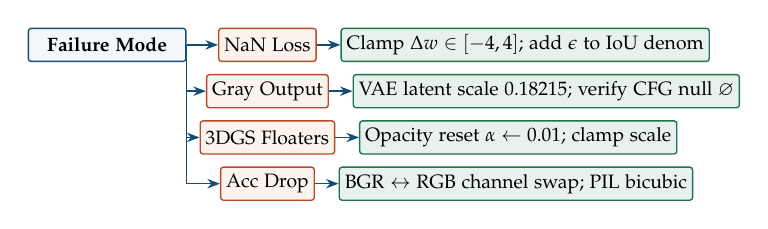
\begin{tikzpicture}[every node/.style={font=\tiny},node distance=1.8mm]
\node[box,draw=acc,fill=soft,minimum width=20mm] (symptom) {\textbf{Failure Mode}};
\node[box,draw=acc2,fill=soft2,right=4mm of symptom] (nan) {NaN Loss};
\node[box,draw=acc2,fill=soft2,below=1.5mm of nan] (gray) {Gray Output};
\node[box,draw=acc2,fill=soft2,below=1.5mm of gray] (needle) {3DGS Floaters};
\node[box,draw=acc2,fill=soft2,below=1.5mm of needle] (drop) {Acc Drop};

\node[box,draw=acc3,fill=acc3!10,right=3mm of nan] (fix1) {Clamp $\Delta w \in [-4, 4]$; add $\epsilon$ to IoU denom};
\node[box,draw=acc3,fill=acc3!10,right=3mm of gray] (fix2) {VAE latent scale $0.18215$; verify CFG null $\varnothing$};
\node[box,draw=acc3,fill=acc3!10,right=3mm of needle] (fix3) {Opacity reset $\alpha \leftarrow 0.01$; clamp scale};
\node[box,draw=acc3,fill=acc3!10,right=3mm of drop] (fix4) {BGR $\leftrightarrow$ RGB channel swap; PIL bicubic};

\draw[arr] (symptom.east) -- (nan.west);
\draw[arr] (symptom.east) |- (gray.west);
\draw[arr] (symptom.east) |- (needle.west);
\draw[arr] (symptom.east) |- (drop.west);

\draw[arr] (nan)--(fix1);
\draw[arr] (gray)--(fix2);
\draw[arr] (needle)--(fix3);
\draw[arr] (drop)--(fix4);
\end{tikzpicture}%
}
\end{center}

\begin{qa}[Production Debugging Scenarios]
\Q{Detection loss suddenly becomes NaN at step 2,400. What is broken and how do you triage?}{
\textbf{Root Causes}:
\begin{itemize}
\item \textbf{Zero-Area Box / Division by Zero}: In GIoU or CIoU, if predicted or ground-truth coordinates satisfy $x_2 \le x_1$ or $y_2 \le y_1$, box area becomes 0 or negative. The enclosing convex hull denominator $|C|$ produces division by zero ($0/0 \to \text{NaN}$).
\item \textbf{Extreme Log Ratio}: If using anchor delta parametrization $\Delta w = \log(w / w_a)$, an unconstrained linear head predicting large positive values (e.g. $+89$) causes $\exp(\Delta w)$ to overflow FP16 max ($65{,}504$).
\end{itemize}
\textbf{The Fix}:
Enforce strict coordinate ordering before loss: $x_1 = \min(x_1, x_2)$, $x_2 = \max(x_1, x_2) + \epsilon$.
Clamp box width/height outputs: $\Delta w = \text{clamp}(\Delta w, \min=-4.0, \max=4.0)$.
Add epsilon ($\epsilon = 10^{-7}$) to all IoU denominators.}
\Q{A ViT model fails to train from scratch on a 50k image dataset (loss plateaus at chance).}{
\textbf{Diagnosis}: Vision Transformers lack 2D local translation and neighborhood inductive biases. On small datasets ($<100\text{k}$ images), random gradient steps in unconstrained self-attention space fail to find spatial structure.
\textbf{The Playbook}:
\begin{enumerate}[leftmargin=*,itemsep=0.8pt]
\item \textbf{Initialize from Pretrained Checkpoints}: Fine-tune from MAE, DINOv2, or ImageNet-21k checkpoints rather than random initialization.
\item \textbf{Inject Heavy Regularization}: If training from scratch is mandatory, implement DeiT's recipe: RandAugment ($N=2, M=9$), Mixup ($\alpha=0.8$), CutMix ($\alpha=1.0$), and Stochastic Depth ($p=0.1$).
\item \textbf{Switch to Hybrid/CNN}: Replace ViT with ConvNeXt-Tiny or Swin-T, whose built-in inductive priors converge reliably on small datasets.
\end{enumerate}}
\Q{Latent Diffusion generates solid grey or noisy static images despite low training loss.}{
\textbf{Diagnosis}:
\begin{enumerate}[leftmargin=*,itemsep=0.8pt]
\item \textbf{Missing VAE Latent Scale}: VAE encoder latents have variance $\approx 5.5$. SD requires scaling latents by $0.18215$ (SDXL: $0.13025$) to enforce unit variance before adding Gaussian noise. Forgetting this leaves signal-to-noise ratio completely mismatched.
\item \textbf{Inverted Timestep Schedule}: Inverting the noise schedule (feeding $t=0$ as pure noise instead of clean image).
\item \textbf{CFG Dropout Bug}: Dropping conditions during training without using the exact same null prompt embedding $\varnothing$ at test time.
\end{enumerate}}
\Q{3D Gaussian Splatting scene produces needle floaters and blurry foreground artifacts.}{
\textbf{Diagnosis}:
Needle floaters stem from Gaussians with one elongated covariance axis ($s_x \gg s_y, s_z$) in unobserved camera frustums.
Blurry foreground stems from failure of adaptive density control to clone under-reconstructed Gaussians.
\textbf{The Fix}:
Clamp maximum spatial scale: $s = \min(s, s_{\text{max}})$.
Enforce \textbf{Periodic Opacity Reset}: Every 3,000 steps, force all Gaussian opacities to near-zero ($\alpha_i \leftarrow 0.01$). Valid surface Gaussians quickly regain opacity from photometric gradients; spurious floaters in empty space remain low and are culled by $\alpha < 0.005$ thresholding.}
\Q{A VLM repeats generated output tokens in an infinite loop during image reasoning.}{
\textbf{Diagnosis}:
\begin{enumerate}
\item \textbf{Visual Attention Sink}: If the projector maps visual tokens to an embedding scale significantly smaller or larger than text token embeddings, attention weights in the LLM backbone saturate on initial visual tokens.
\item \textbf{Missing End-of-Sequence (EOS) Supervision}: Pretraining data omitted \texttt{<|im\_end|>} or \texttt{</s>} tokens, teaching the LLM to continue emitting tokens forever.
\end{enumerate}
\textbf{The Fix}: Add LayerNorm at projector exit to equalize visual and text embedding variance; enforce repetition penalties during decoding; audit presence of EOS tokens in instruction tuning targets.}
\Q{Validation accuracy drops 25\% on deployed model despite zero change in weights.}{
\textbf{Triage Checklist}:
\begin{enumerate}
\item \textbf{Color Channel Swap}: Check if deployed inference feeds OpenCV BGR into a model trained on Torchvision RGB.
\item \textbf{Resizing Interpolation}: Training used PIL bicubic with antialiasing; deployed engine used \lstinline|INTER_NEAREST| or \lstinline|INTER_LINEAR|.
\item \textbf{Normalization Mean/Std}: Input was scaled to $[0, 1]$ but omitted ImageNet subtract mean and divide std.
\end{enumerate}}
\end{qa}

\section{Rapid-Fire Q\&A and Vision Glossary}\label{sec:rapid}
\lab{Rapid interview drills \textperiodcentered\ core definitions \textperiodcentered\ precise terminology}

\subsection{Rapid-Fire Drills (Answer in under 5 seconds)}
\RF{Why use $1\times 1$ convs in ResNet bottleneck?}{Changes channel dimension cheaply without changing spatial resolution.}
\RF{What does RoIAlign do that RoIPool didn't?}{Eliminates coordinate quantization using 4-point bilinear interpolation.}
\RF{Why do ViTs need positional embeddings?}{Self-attention is permutation-equivariant; without PosEnc, patches have no spatial order.}
\RF{What is the FLOP cost of a 2D convolution?}{$2 \cdot C_{\text{in}} \cdot C_{\text{out}} \cdot K^2 \cdot H_o W_o$.}
\RF{Why does SigLIP scale better than CLIP?}{Replaces global softmax with pairwise sigmoid loss, eliminating cross-GPU all-gather.}
\RF{What is the patch count for $384\times 384$ at $P=16$?}{$(384/16)^2 = 24^2 = 576$ tokens.}
\RF{What is the spatial compression of standard SD VAE?}{$8\times$ in height and width ($64\times$ area compression).}
\RF{What target does Flow Matching predict?}{Constant velocity vector field $v_t = x_1 - x_0$.}
\RF{What is transmittance in NeRF?}{Probability that a light ray travels from $t_n$ to $t$ without colliding with particles.}
\RF{How many floats represent a 3D Gaussian in 3DGS?}{59 floats: 3 position, 3 scale, 4 quaternion, 1 opacity, 48 spherical harmonics.}
\RF{What is Focal Loss's focusing parameter?}{$\gamma$ (typically $\gamma=2$), which exponentially downweights easy negatives.}
\RF{Why does MAE mask 75\% of patches?}{Images have high spatial redundancy; high masking prevents trivial pixel interpolation.}
\RF{What does DINO self-attention map capture?}{Unsupervised semantic segmentation masks of foreground objects.}
\RF{What causes object hallucination in VLMs?}{Language priors from text pretraining overpowering visual token attention.}
\RF{How is Panoptic Quality calculated?}{$\text{PQ} = \text{SQ} \times \text{RQ}$ (Segmentation Quality $\times$ Recognition Quality).}
\RF{What is the difference between SIFT and ORB?}{SIFT uses floating-point DoG histograms; ORB uses FAST corners and binary BRIEF strings.}
\RF{What is the epipolar line equation?}{$l' = \mathbf{F} x$, where $\mathbf{F}$ is the Fundamental Matrix.}
\RF{Why is the linear bottleneck in MobileNetV2 linear?}{ReLU non-linearities in low-dimensional manifolds collapse and zero out features.}
\RF{What is the formula for the Canny gradient direction?}{$\theta = \arctan(G_y / G_x)$, quantized into $0^\circ, 45^\circ, 90^\circ, 135^\circ$.}
\RF{What is the purpose of adaLN-Zero in DiT?}{Initializes scale gating to zero so every block acts as identity at step 0.}

\subsection{The Vision Glossary}
\begin{description}[leftmargin=1.2em,itemsep=1.5pt]
\item[\textbf{Anchor Box}] Pre-defined candidate bounding box with fixed scale and aspect ratio used in detectors like Faster R-CNN and YOLOv3.
\item[\textbf{ASPP}] Atrous Spatial Pyramid Pooling; parallel atrous convolutions with diverse dilation rates capturing multi-scale context.
\item[\textbf{BEV (Bird's-Eye-View)}] Top-down 2D coordinate representation of 3D scenes used in autonomous driving perception.
\item[\textbf{CFG (Classifier-Free Guidance)}] Diffusion sampling technique extrapolating conditional over unconditional predictions: $\epsilon_\varnothing + s(\epsilon_c - \epsilon_\varnothing)$.
\item[\textbf{Deformable Conv}] Convolution where 2D sampling grid offsets are predicted dynamically from input features.
\item[\textbf{DLT (Direct Linear Transformation)}] Linear algorithm for solving projective camera and homography matrices from point correspondences.
\item[\textbf{Epipolar Plane}] 3D plane formed by a 3D scene point and the two camera optical centers.
\item[\textbf{FPN (Feature Pyramid Network)}] Top-down architecture with lateral skip connections combining multi-scale semantic and spatial features.
\item[\textbf{GIoU (Generalized IoU)}] IoU metric penalized by normalized empty space within the smallest enclosing bounding box.
\item[\textbf{Homography}] $3\times 3$ projective transformation mapping coplanar 3D points between two camera views: $x' \sim Hx$.
\item[\textbf{Inverted Residual}] Block structure expanding channels with $1\times 1$ conv before $3\times 3$ depthwise conv, ending with linear bottleneck.
\item[\textbf{LPIPS}] Learned Perceptual Image Patch Similarity; distance between deep feature activations from a pretrained VGG network.
\item[\textbf{NMS (Non-Maximum Suppression)}] Greedy algorithm pruning overlapping bounding boxes based on IoU thresholding.
\item[\textbf{Patchify}] Splitting a 2D image into non-overlapping grid tiles and linearly projecting them to 1D token embeddings.
\item[\textbf{RoIAlign}] Bilinear interpolation sampling inside region of interest bins to preserve floating-point spatial alignment.
\item[\textbf{Spherical Harmonics (SH)}] Orthogonal basis functions on the 2D sphere modeling view-dependent radiance in NeRF and 3DGS.
\item[\textbf{Swin Window Attention}] Restricting self-attention to localized $M\times M$ patch windows with linear complexity $\mathcal{O}(N)$.
\item[\textbf{Transmittance}] Accumulation of transparency along a camera ray in volumetric rendering: $T(t) = \exp(-\int \sigma ds)$.
\item[\textbf{VQ-VAE}] Vector Quantized Variational Autoencoder mapping continuous image latents to discrete codebook indices.
\end{description}

\section{High-Velocity Vision Interview Drill}\label{sec:rapid2}
\lab{20 rapid-fire technical questions \textperiodcentered\ flashcards \textperiodcentered\ edge cases \textperiodcentered\ instant answers}

\begin{qa}[Rapid-Fire Architecture \& Mechanics Drills]
\RF{Why do ViTs fail when trained from scratch on small datasets without pretraining?}{ViTs lack the inductive biases of convolutions (translation equivariance and local spatial locality); they must learn spatial relationships from scratch via massive data.}
\RF{How do you resize learned 2D positional embeddings when fine-tuning a ViT at higher resolution?}{Bicubic 2D spatial interpolation on the $(H/P) \times (W/P)$ position grid, leaving the [CLS] embedding unchanged.}
\RF{What is the purpose of the hard distillation token in DeiT?}{It interacts with patch tokens and [CLS] via self-attention, but its loss is trained exclusively against the hard class labels predicted by a teacher ConvNet (RegNet).}
\RF{Why does Soft-NMS outperform standard Hard-NMS in dense crowd scenes?}{Hard-NMS instantly zeros the score of overlapping boxes, destroying true overlapping objects; Soft-NMS smoothly decays the score using a Gaussian or linear penalty: $s_i \leftarrow s_i \exp(-\frac{\text{IoU}^2}{\sigma})$.}
\RF{Why does ASPP in DeepLab use atrous (dilated) convolutions instead of pooling?}{Dilated convolutions expand the receptive field to capture multi-scale context without downsampling spatial resolution or losing fine-grained edge localization.}
\RF{What is the Degenerate Grid trap in large atrous convolution dilation rates?}{When dilation rate $r$ approaches feature map size $W$, a $3 \times 3$ kernel samples outside bounds or only isolated pixels, degenerating into a trivial $1 \times 1$ convolution.}
\RF{Why can't BatchNorm be used directly in Vision Transformers?}{Batch statistics fluctuate excessively across sequence lengths, and ViT token representations undergo covariate shifts along sequence dimensions; LayerNorm normalizes across feature channels per token independently.}
\RF{What is the difference between Transposed Convolution and Bilinear Upsampling?}{Transposed convolutions learn upsampling weights but suffer from "checkerboard artifacts" when stride does not divide kernel size; Bilinear upsampling is non-parametric, smooth, and artifact-free.}
\RF{Why does CLIP require a learned temperature parameter $\tau$?}{Cosine similarities lie in $[-1, 1]$; with 32k negatives the softmax over such logits is almost uniform (the positive gets at most $e^{1}/(e^{1} + 32767\,e^{-1}) \approx 0.02\%$). Dividing by $\tau \approx 0.07$ stretches logits to $[-14, 14]$ so the positive can win.}
\RF{What is the All-Gather gradient bottleneck in distributed CLIP?}{\texttt{all\_gather} is not differentiable, so gathered negatives carry no gradient. Fix: replace your own rank's slice with the local tensor (keeps its gradient), or use a differentiable gather and compute only the local rows of the logit matrix (OpenCLIP \texttt{local\_loss}).}
\RF{Why does Min-SNR $\gamma$ loss weighting improve diffusion model convergence?}{Diffusion loss at small $t$ has massive SNR and over-supervises high-frequency noise; clamping loss weight $\min(\text{SNR}(t), \gamma)$ balances gradient contributions across all timesteps.}
\RF{What is the difference between DDPM and DDIM sampling?}{DDPM is a stochastic Markov chain requiring 1000 steps; DDIM defines an equivalent non-Markovian process whose deterministic ODE allows skipping steps in 20--50 iterations.}
\RF{Why does Flow Matching use straight trajectories instead of curved Brownian paths?}{Straight ODE paths minimize displacement length between noise and data, resulting in velocity fields that are nearly constant in time, enabling 1-step or 4-step Euler integration.}
\RF{Why does NeRF require Hierarchical Volume Sampling (Coarse and Fine networks)?}{Uniform ray sampling wastes $90\%$ of MLP evaluations in empty space or occluded regions; the coarse network generates a probability density function along the ray to concentrate fine samples around surfaces.}
\RF{Why does 3DGS use Spherical Harmonics instead of a tiny MLP for color?}{Spherical Harmonics evaluate in closed form via direct polynomial multiplication ($<0.1\,\mu$s on CUDA), whereas evaluating an MLP per Gaussian would bottleneck real-time 100+ FPS rendering.}
\RF{How does ByteTrack track occluded and low-confidence detections?}{Instead of discarding boxes with confidence $<0.5$, ByteTrack matches high-confidence boxes first, then runs a second association matching low-confidence boxes to unmatched tracklets.}
\RF{What is the difference between Post-Training Quantization (PTQ) and QAT?}{PTQ quantizes frozen FP32 weights using a calibration dataset without backpropagation ($\sim$minutes); QAT simulates fake-quantization during retraining with straight-through estimator ($\sim$days).}
\RF{What is the aperture problem in optical flow?}{Through a small aperture (local window), motion parallel to an edge cannot be detected; only normal motion perpendicular to the gradient is measurable.}
\RF{Why does Mask2Former unify semantic, instance, and panoptic segmentation?}{It treats all segmentation tasks as binary mask prediction with query-based cross-attention constrained inside predicted mask regions (Masked Attention).}
\RF{What is the difference between Epipolar Line and Epipole?}{The epipole is the projection of the other camera center onto the image plane; the epipolar line is the intersection of the epipolar plane with the image plane, upon which all matching points must lie.}
\end{qa}

\begin{trap}[Crucial Interview Traps \& Failure Modes]
\begin{itemize}
\item \textbf{ViT Quadratic Complexity Assumption}: Candidates often say "ViT is always $\mathcal{O}(N^2)$". FlashAttention still does $\mathcal{O}(N^2)$ FLOPs but never materializes the $N\times N$ matrix, so memory is $\mathcal{O}(N)$ and it runs several times faster; only windowed (Swin) or linear attention changes the FLOP scaling.
\item \textbf{Assuming Diffusion Directly Predicts the Clean Image $x_0$}: Predicting noise $\epsilon_t$ or velocity $v_t$ is dramatically more numerically stable than predicting clean image $x_0$, because at large $t$, $x_0$ has near-zero signal-to-noise ratio and predicting it causes blurry mean-image collapse.
\item \textbf{Overlooking Bounding Box Coordinate Normalization}: Feeding absolute pixel coordinates $(x, y, w, h)$ into loss functions rather than normalized $[0, 1]$ coordinates breaks scale-invariance across different image sizes.
\end{itemize}
\end{trap}

\section{Master Vision Formula Sheet}\label{sec:formulas}
\lab{Convolution \textperiodcentered\ receptive field \textperiodcentered\ attention FLOPs \textperiodcentered\ geometry \textperiodcentered\ detection \textperiodcentered\ diffusion \textperiodcentered\ 3DGS}

\noindent\begin{tabularx}{\linewidth}{@{}p{23mm} X@{}}
\toprule
\textbf{Mechanism} & \textbf{Mathematical Formulation \& Invariants}\\
\midrule
\textbf{Conv2D Output} & $O = \lfloor \frac{I - K + 2P}{S} \rfloor + 1$ \quad (dilation $d \implies K' = K + (K-1)(d-1)$)\\
\textbf{Conv2D FLOPs} & $\text{FLOPs} = 2 \cdot C_{\text{in}} \cdot C_{\text{out}} \cdot K^2 \cdot H_{\text{out}} \cdot W_{\text{out}}$\\
\textbf{Receptive Field} & $RF_l = RF_{l-1} + (K_l - 1) \cdot J_{l-1}, \quad J_l = J_{l-1} \cdot S_l$\\
\textbf{Depthwise Ratio} & $\frac{\text{FLOPs}_{\text{sep}}}{\text{FLOPs}_{\text{std}}} = \frac{1}{C_{\text{out}}} + \frac{1}{K^2} \approx \frac{1}{9} \quad (\text{for } 3\times 3, C_{\text{out}} \gg 1)$\\
\textbf{Standard ViT Attn} & $\Omega(\text{MSA}) = 4ND^2 + 2N^2D, \quad \Omega(\text{MLP}) = 8ND^2$\\
\textbf{Swin Window Attn} & $\Omega(\text{W-MSA}) = 4ND^2 + 2M^2ND \quad (\text{linear in } N, M=7)$\\
\textbf{Harris Response} & $R = \det(M) - k \cdot (\operatorname{Tr}(M))^2 = \lambda_1 \lambda_2 - k(\lambda_1 + \lambda_2)^2$\\
\textbf{Optical Flow} & $I_x u + I_y v + I_t = 0 \iff \nabla I^T \mathbf{v} + I_t = 0 \quad (\text{Aperture})$\\
\textbf{Epipolar Line} & $x_2^T F x_1 = 0 \quad (\text{uncalibrated } F), \quad \hat{x}_2^T E \hat{x}_1 = 0 \quad (E)$\\
\textbf{RANSAC Count} & $N = \frac{\ln(1 - p)}{\ln(1 - (1 - \epsilon)^s)} \quad (\text{sample } s, \text{ outlier ratio } \epsilon)$\\
\textbf{Focal Loss} & $\text{FL}(p_t) = -\alpha_t (1 - p_t)^\gamma \log(p_t) \quad (\gamma=2.0, \alpha_t=0.25)$\\
\textbf{CIoU Loss} & $\mathcal{L}_{\text{CIoU}} = 1 - \text{IoU} + \frac{\rho^2(\mathbf{b}, \mathbf{b}^{\text{gt}})}{c^2} + \alpha v$\\[1pt]
& $v = \frac{4}{\pi^2}\left(\arctan\frac{w^{\text{gt}}}{h^{\text{gt}}} - \arctan\frac{w}{h}\right)^2$\\
\textbf{TAL Metric} & $t = s^\alpha \times \text{IoU}^\beta \quad (\alpha=0.5, \beta=6.0\text{ in YOLOv8/v11})$\\
\textbf{CLIP InfoNCE} & $\mathcal{L} = -\frac{1}{2B}\sum_{i=1}^B \left[ \log\frac{e^{S_{ii}/\tau}}{\sum_j e^{S_{ij}/\tau}} + \log\frac{e^{S_{ii}/\tau}}{\sum_j e^{S_{ji}/\tau}} \right]$\\
\textbf{SigLIP Loss} & $\mathcal{L} = -\frac{1}{B}\sum_{i,j} \log \sigma\left( y_{ij} (I_i^T T_j \cdot e^t + b) \right), \, y_{ij} \in \{\pm 1\}$\\
\textbf{DDPM Noising} & $x_t = \sqrt{\bar{\alpha}_t} x_0 + \sqrt{1 - \bar{\alpha}_t} \epsilon, \quad \bar{\alpha}_t = \prod_{s=1}^t (1 - \beta_s)$\\
\textbf{CFG Score} & $\tilde{\epsilon}_\theta(x_t, c) = \epsilon_\theta(x_t, \varnothing) + s \cdot (\epsilon_\theta(x_t, c) - \epsilon_\theta(x_t, \varnothing))$\\
\textbf{Rectified Flow} & $x_t = (1 - t) x_0 + t x_1, \quad \frac{d x_t}{dt} = v_t = x_1 - x_0$\\
\textbf{NeRF Quadrature} & $C(\mathbf{r}) = \int_{t_n}^{t_f} T(t) \sigma(\mathbf{r}(t)) \mathbf{c}(\mathbf{r}(t), \mathbf{d})\, dt$\\[1pt]
& $T(t) = \exp\left(-\int_{t_n}^t \sigma(\mathbf{r}(s))\, ds\right)$\\
\textbf{3DGS Projected Cov} & $\mathbf{\Sigma}' = \mathbf{J} \mathbf{W} \mathbf{\Sigma} \mathbf{W}^T \mathbf{J}^T + 0.3 \cdot \mathbf{I}_{2 \times 2}, \quad \mathbf{\Sigma} = \mathbf{R} \mathbf{S} \mathbf{S}^T \mathbf{R}^T$\\
\textbf{Panoptic Quality} & $\text{PQ} = \frac{\sum_{\text{TP}} \text{IoU}}{|\text{TP}| + \frac{1}{2}|\text{FP}| + \frac{1}{2}|\text{FN}|} = \text{SQ} \times \text{RQ}$\\
\textbf{FID Score} & $\text{FID} = \|\mu_r - \mu_g\|_2^2 + \operatorname{Tr}\left( \mathbf{\Sigma}_r + \mathbf{\Sigma}_g - 2(\mathbf{\Sigma}_r \mathbf{\Sigma}_g)^{1/2} \right)$\\
\textbf{Conv-BN Folding} & $W_{\text{fused}} = \frac{\gamma}{\sqrt{\sigma^2 + \epsilon}} W, \quad b_{\text{fused}} = \frac{\gamma}{\sqrt{\sigma^2 + \epsilon}} (b - \mu) + \beta$\\
\bottomrule
\end{tabularx}

\section{30 Seminal Vision Papers}\label{sec:papers}
\lab{Foundational papers \textperiodcentered\ Authors \& Year \textperiodcentered\ Breakthroughs \textperiodcentered\ Paradigms}

\begin{enumerate}[leftmargin=*,itemsep=0.5pt,topsep=1pt]
\item \textbf{AlexNet} (Krizhevsky et al., 2012): Deep convolutional network with ReLU, Dropout, and GPU parallelization; shattered ImageNet error from 26\% to 16\%, launching deep learning.
\item \textbf{VGG} (Simonyan \& Zisserman, 2014): Proved that deep stacks of small $3\times 3$ convs outperform wide filters ($7\times 7$), establishing modern homogeneous ConvNet architecture.
\item \textbf{ResNet} (He et al., 2015): Residual identity shortcuts solving vanishing gradients up to 152 layers ($\mathcal{H}(x) = \mathcal{F}(x) + x$), winner of ImageNet, COCO, and ILSVRC 2015.
\item \textbf{U-Net} (Ronneberger et al., 2015): Symmetric encoder-decoder architecture with cross-skip concatenation preserving spatial details for dense pixel-level medical segmentation.
\item \textbf{Faster R-CNN} (Ren et al., 2015): First end-to-end deep detector; introduced Region Proposal Networks (RPN) sharing convolutional features with Fast R-CNN detector.
\item \textbf{Mask R-CNN} (He et al., 2017): RoIAlign with bilinear interpolation eliminating sub-pixel quantization; parallel FCN branch adding instance segmentation to object detection.
\item \textbf{RetinaNet} (Lin et al., 2017): Focal loss solving extreme 1000:1 foreground-background class imbalance, enabling single-stage detectors to match two-stage accuracy.
\item \textbf{MobileNetV2} (Sandler et al., 2018): Inverted residuals and linear bottlenecks preserving manifold capacity in low-dimensional space for mobile inference.
\item \textbf{YOLO Family} (Redmon 2016 / Jocher 2023): Real-time single-stage detection evolving from grid regression (v1) to CSPNet (v5) and anchor-free TAL + DFL heads (v8/v11).
\item \textbf{DETR} (Carion et al., 2020): Reformulated object detection as direct set prediction using Transformers and Hungarian bipartite matching, completely eliminating hand-crafted NMS.
\item \textbf{ViT} (Dosovitskiy et al., 2020): Proved standard Transformer applied directly to sequences of $16\times 16$ image patches attains SOTA ImageNet accuracy when pretrained on large data (JFT-300M).
\item \textbf{Deformable DETR} (Zhu et al., 2020): Replaced global attention with multi-scale deformable attention sampling $K=4$ sparse points per query, accelerating convergence by $10\times$.
\item \textbf{Swin Transformer} (Liu et al., 2021): Shifted Window self-attention achieving linear computational complexity $\mathcal{O}(N)$ and hierarchical multi-scale representations for dense vision.
\item \textbf{SimCLR} (Chen et al., 2020): Contrastive self-supervised learning with normalized InfoNCE loss, stochastic data augmentations, and non-linear projection MLP heads.
\item \textbf{MAE} (He et al., 2021): Masked Autoencoders masking $75\%$ of visual patches with an asymmetric encoder-decoder, demonstrating that autoencoding is scalable self-supervision for vision.
\item \textbf{DINO / DINOv2} (Caron 2021 / Oquab 2023): Self-distillation without labels via centering and sharpening; produces emergent semantic part segmentations and foundation visual representations.
\item \textbf{CLIP} (Radford et al., 2021): Contrastive Language-Image Pretraining on 400M web image-text pairs; enables zero-shot classification via natural language prompting.
\item \textbf{SigLIP} (Zhai et al., 2023): Sigmoid pairwise loss eliminating all-gather softmax normalization across distributed GPUs, scaling dual-encoder training to million-scale batch sizes.
\item \textbf{ConvNeXt-V2} (Woo et al., 2023): Modernized pure ConvNet with 7x7 depthwise kernels and Global Response Normalization (GRN), outperforming Swin on ImageNet and COCO.
\item \textbf{DDPM} (Ho et al., 2020): Denoising Diffusion Probabilistic Models establishing connection between diffusion probabilistic models and score-based denoising score matching.
\item \textbf{Latent Diffusion / Stable Diffusion} (Rombach et al., 2022): Moved diffusion into perceptual $f=8$ latent space of a pretrained VAE, reducing compute by orders of magnitude.
\item \textbf{DiT} (Peebles \& Xie, 2023): Diffusion Transformer replacing U-Net with ViT and adaLN-Zero modulation, establishing compute scaling laws for visual generative models.
\item \textbf{Flow Matching / Rectified Flow} (Lipman 2022 / Liu 2022): Straight continuous probability trajectories predicting constant velocity $v_t = x_1 - x_0$, enabling 1--4 step generation.
\item \textbf{SAM / SAM 2} (Kirillov 2023 / Ravi 2024): Foundation promptable segmentation models; SA-1B dataset; streaming memory bank for real-time video object segmentation.
\item \textbf{NeRF} (Mildenhall et al., 2020): Neural Radiance Fields synthesizing photorealistic novel views via 5D coordinate MLPs and differentiable volumetric rendering.
\item \textbf{3D Gaussian Splatting} (Kerbl et al., 2023): Replaced coordinate MLPs with explicit 3D Gaussians and tile-based rasterization, achieving photorealistic novel-view synthesis at $>100$ FPS.
\item \textbf{LLaVA / LLaVA-NeXT} (Liu 2023 / Liu 2024): Visual instruction tuning using CLIP and LLaMA backbones; AnyRes dynamic grid slicing for high-resolution document parsing.
\item \textbf{Qwen2-VL} (Wang et al., 2024): Native dynamic resolution VLM with 2D/3D visual RoPE, eliminating aspect ratio distortion and fixed grid constraints.
\item \textbf{Flux.1} (Black Forest Labs, 2024): 12B parameter Flow Matching generative model with rectified flow ODEs and multimodal double-stream transformer blocks.
\item \textbf{Sora} (OpenAI, 2024): Spacetime diffusion transformer operating on 3D video patches, scaling video generation across diverse durations, resolutions, and aspect ratios.
\end{enumerate}

\section{References: The Vision Canon}\label{sec:refs}
{\small\raggedright
\newcommand{\rf}[2]{\par\noindent\hangindent=1em\hangafter=1 #1 {\color{mute}\ttfamily\scriptsize #2}\par}

\paragraph{Classical Geometry, Filtering \& Flow (1, 1b)}
\rf{Hartley \& Zisserman 2004, \emph{Multiple View Geometry in Computer Vision}.}{Cambridge Univ Press}
\rf{Lowe 2004, \emph{Distinctive Image Features from Scale-Invariant Keypoints} (SIFT).}{IJCV 60(2)}
\rf{Rublee et al.\ 2011, \emph{ORB: An efficient alternative to SIFT or SURF}.}{ICCV 2011}
\rf{Lucas \& Kanade 1981; Horn \& Schunck 1981, \emph{Determining Optical Flow}.}{AI Journal}
\rf{Teed \& Deng 2020, \emph{RAFT: Recurrent All-Pairs Field Transforms for Optical Flow}.}{2003.12039}

\paragraph{Convolutions \& Modern Backbones (2, 2b)}
\rf{He et al.\ 2016, \emph{Deep Residual Learning for Image Recognition} (ResNet).}{1512.03385}
\rf{Sandler et al.\ 2018, \emph{MobileNetV2: Inverted Residuals and Linear Bottlenecks}.}{1801.04381}
\rf{Ma et al.\ 2018, \emph{ShuffleNet V2: Practical Guidelines for Efficient CNN Architecture}.}{1807.11164}
\rf{Tan \& Le 2019, \emph{EfficientNet: Rethinking Model Scaling for CNNs}.}{1905.11946}
\rf{Liu et al.\ 2022, \emph{A ConvNet for the 2020s} (ConvNeXt); Woo et al.\ 2023 (ConvNeXt-V2).}{2201.03545, 2301.00808}

\paragraph{Vision Transformers \& Hierarchical ViTs (3, 4)}
\rf{Dosovitskiy et al.\ 2020, \emph{An Image is Worth 16x16 Words} (ViT).}{2010.11929}
\rf{Touvron et al.\ 2021, \emph{Training data-efficient image transformers} (DeiT).}{2012.12877}
\rf{Liu et al.\ 2021, \emph{Swin Transformer: Hierarchical Vision Transformer using Shifted Windows}.}{2103.14030}
\rf{Dehghani et al.\ 2023, \emph{Scaling Vision Transformers to 22 Billion Parameters} (ViT-22B).}{2302.05442}
\rf{Dehghani et al.\ 2023, \emph{Patch n' Pack: NaViT, a Vision Transformer for any Aspect Ratio}.}{2307.06304}

\paragraph{Object Detection \& Set Prediction (5, 5b, 6)}
\rf{Ren et al.\ 2015, \emph{Faster R-CNN}; He et al.\ 2017, \emph{Mask R-CNN}.}{1506.01497, 1703.06870}
\rf{Lin et al.\ 2017, \emph{Focal Loss for Dense Object Detection} (RetinaNet).}{1708.02002}
\rf{Carion et al.\ 2020, \emph{End-to-End Object Detection with Transformers} (DETR).}{2005.12872}
\rf{Zhu et al.\ 2020, \emph{Deformable DETR}; Zhang et al.\ 2022, \emph{DINO-DETR}.}{2010.04159, 2203.03605}
\rf{Wang et al.\ 2024, \emph{YOLOv10: Real-Time End-to-End Object Detection}.}{2405.14458}

\paragraph{Segmentation \& Foundation Models (7, 7b)}
\rf{Ronneberger et al.\ 2015, \emph{U-Net: Convolutional Networks for Biomedical Segmentation}.}{1505.04597}
\rf{Chen et al.\ 2017, \emph{Rethinking Atrous Convolution for Semantic Image Segmentation} (DeepLabv3).}{1706.05587}
\rf{Cheng et al.\ 2022, \emph{Masked-attention Mask Transformer for Universal Segmentation} (Mask2Former).}{2112.01527}
\rf{Kirillov et al.\ 2023, \emph{Segment Anything} (SAM); Ravi et al.\ 2024 (SAM 2).}{2304.02643, 2408.00714}

\paragraph{Self-Supervised Learning \& Dual Encoders (8, 8b, 9)}
\rf{Chen et al.\ 2020, \emph{A Simple Framework for Contrastive Learning} (SimCLR); He 2020 (MoCo).}{2002.05709, 1911.05722}
\rf{He et al.\ 2021, \emph{Masked Autoencoders Are Scalable Vision Learners} (MAE).}{2111.06377}
\rf{Caron et al.\ 2021, \emph{Emerging Properties in Self-Supervised ViTs} (DINO); Oquab 2023 (DINOv2).}{2104.14294, 2304.07193}
\rf{Radford et al.\ 2021, \emph{Learning Transferable Visual Models} (CLIP).}{2103.00020}
\rf{Zhai et al.\ 2023, \emph{Sigmoid Loss for Language-Image Pre-Training} (SigLIP).}{2303.15343}

\paragraph{Generative Diffusion, DiT \& Flow Matching (11, 12, 13)}
\rf{Ho et al.\ 2020, \emph{DDPM}; Song et al.\ 2020, \emph{Score SDE}; Song et al.\ 2020, \emph{DDIM}.}{2006.11239, 2011.13456, 2010.02502}
\rf{Karras et al.\ 2022, \emph{Elucidating the Design Space of Diffusion} (EDM).}{2206.00364}
\rf{Rombach et al.\ 2022, \emph{High-Resolution Image Synthesis with Latent Diffusion Models}.}{2112.10752}
\rf{Peebles \& Xie 2023, \emph{Scalable Diffusion Models with Transformers} (DiT).}{2212.09748}
\rf{Lipman et al.\ 2022, \emph{Flow Matching for Generative Modeling}; Liu 2022 (Flow Straight and Fast).}{2210.02747, 2209.03003}
\rf{Esser et al.\ 2024, \emph{Scaling Rectified Flow Transformers for High-Res Synthesis} (SD3 MM-DiT).}{2403.03206}

\paragraph{Video Foundations, 3D \& Multimodal LLMs (10, 10b, 14, 15, 15b)}
\rf{Mildenhall et al.\ 2020, \emph{NeRF}; Kerbl et al.\ 2023, \emph{3D Gaussian Splatting}.}{2003.08934, 2308.04079}
\rf{Bertasius et al.\ 2021, \emph{TimeSformer}; Brooks et al.\ 2024 (Sora Technical Report).}{2102.05095, openai.com}
\rf{Liu et al.\ 2023, \emph{LLaVA}; Wang et al.\ 2024, \emph{Qwen2-VL: To See the World More Clearly}.}{2304.08485, 2409.12191}
\rf{Li et al.\ 2023, \emph{Evaluating Object Hallucination in Large Vision-Language Models} (POPE).}{2305.10355}
\rf{Leng et al.\ 2024, \emph{Mitigating Object Hallucination via Visual Contrastive Decoding} (VCD).}{2311.16922}
\rf{Frossard et al.\ 2024, \emph{ColPali: Efficient Document Retrieval with Vision Language Models}.}{2407.01449}
\rf{Li et al.\ 2022, \emph{BEVFormer: Learning BEV Representation with Spatiotemporal Transformers}.}{2203.17270}
\rf{Zhang et al.\ 2022, \emph{ByteTrack: Multi-Object Tracking by Associating Every Detection Box}.}{2110.06864}
}

\section{The 21-Day Vision Mastery Curriculum}\label{sec:plan}
\lab{Foundations \textperiodcentered\ Multimodal \& Generative \textperiodcentered\ Systems \& Edge \textperiodcentered\ Code-Blind \textperiodcentered\ Mock Rubrics}

\begin{mem}[The 3-Phase Revision Architecture]
\begin{tabularx}{\columnwidth}{@{}l l X@{}}
\toprule
\textbf{Phase} & \textbf{Days} & \textbf{Core Focus \& Daily Target} \\
\midrule
\textbf{Phase 1} & Days 1--7 & \textbf{Foundations}: Classical CV, CNNs, ViTs, Detection, SAM, SSL \\
\textbf{Phase 2} & Days 8--14 & \textbf{Generative \& 3D}: CLIP, VLMs, Diffusion, Flow, Video, 3DGS \\
\textbf{Phase 3} & Days 15--21 & \textbf{Systems \& Drills}: Metrics, Edge NPU, Code-Blind, Mock Interviews \\
\bottomrule
\end{tabularx}
\end{mem}

\subsection*{Day-by-Day Execution Schedule}
\begin{itemize}[leftmargin=*,itemsep=0.8pt]
\item \textbf{Days 1--2 (Classical \& Convolutions)}: Derive Harris response $R$ and Hartley 8-point normalization; calculate RANSAC sample count ($N=72$ for $\epsilon=0.5$); compute Conv2D output shape and receptive field recurrence ($RF_l = RF_{l-1} + (K-1)J$); derive depthwise separable FLOP ratio ($\sim 1/9$); explain ConvNeXt-V2 GRN.
\item \textbf{Days 3--4 (ViTs \& Single-Stage Detectors)}: Derive ViT self-attention FLOPs ($4ND^2 + 2N^2D$); trace DeiT distillation token and Swin cyclic shift masking; derive Focal Loss gradient suppression ($10,000\times$ on easy negatives); compare RoIPool vs RoIAlign; analyze YOLOv8/v11 TAL metric ($s^\alpha \cdot \text{IoU}^\beta$) and DFL distribution regression.
\item \textbf{Days 5--6 (DETR \& Segmentation)}: Trace DETR Hungarian bipartite assignment; calculate Deformable Attention sampling complexity ($4MK$ vs $N$); analyze DINO-DETR contrastive denoising; compare DeepLabv3+ ASPP to Mask2Former masked attention; walk through SAM ViT-H windowed backbone and SAM 2 streaming video memory bank.
\item \textbf{Day 7 (Self-Supervised Learning)}: Prove InfoNCE lower bound on mutual information; analyze BYOL non-collapse dynamics; explain MAE $75\%$ masking asymmetric speedup and DINOv2 KoLeo entropy regularization with register tokens.
\item \textbf{Days 8--9 (CLIP \& Multimodal LLMs)}: Derive CLIP InfoNCE gradients and distributed All-Gather backward bottleneck; compare CLIP softmax vs SigLIP pairwise sigmoid loss; diagram LLaVA AnyRes grid slicing; analyze Qwen2-VL native 2D/3D RoPE; explain POPE splits and VCD contrastive decoding.
\item \textbf{Days 10--11 (Diffusion Foundations \& DiT)}: Derive DDPM forward noising $x_t = \sqrt{\bar{\alpha}_t} x_0 + \sqrt{1-\bar{\alpha}_t}\epsilon$; connect score matching to Tweedie's formula; analyze EDM continuous $\sigma$ scaling and CFG burn; contrast pixel diffusion vs latent VAE ($f=8$); trace DiT adaLN-Zero compute scaling laws.
\item \textbf{Days 12--13 (Flow Matching \& Video Models)}: Derive straight probability trajectories and constant velocity objective $v_t = x_1 - x_0$; explain 2-Rectified Flow Reflowing; contrast Flux.1 double vs single stream blocks; factorize 3D attention into spatial-then-temporal operations; prove $15\times$ memory reduction; analyze Sora spacetime patch grids.
\item \textbf{Day 14 (3D NeRF \& Gaussian Splatting)}: Derive NeRF volumetric quadrature rendering; prove 3D covariance positive semi-definiteness ($\Sigma = R S S^T R^T$); trace 3DGS tile rasterizer with 64-bit Radix sort and EWA Jacobian projection.
\item \textbf{Days 15--16 (Benchmarks \& Edge Deployment)}: Calculate Panoptic Quality $\text{PQ} = \text{SQ} \times \text{RQ}$; derive FID 2-Wasserstein distance under Gaussian assumption; evaluate POPE Yes-ratio and MMBench circular eval; derive Conv-BN folding; explain TensorRT INT8 calibration via KL divergence minimization; trace ByteTrack secondary association.
\item \textbf{Days 17--18 (System Design \& Code-Blind)}: Architect autonomous vehicle 3D perception (BEVFormer); design ColPali late-interaction visual document retrieval; write blind in $<5$ minutes: Conv2D via \texttt{im2col}, ResNet Bottleneck, ViT PatchEmbed, 2D RoPE, InfoNCE loss, and Vectorized NMS.
\item \textbf{Days 19--20 (Training Loops \& Napkin Math)}: Write pure PyTorch execution loops for SimCLR step, DDPM step, Rectified Flow step, and AnyRes image slicer; compute without calculator: Conv FLOPs, ViT quadratic memory, distributed CLIP network bandwidth, 3DGS VRAM footprint, and edge NPU FPS.
\item \textbf{Day 21 (Final Rapid-Fire Drill)}: Fire through all 40 rapid-fire flashcards aloud; time each answer strictly under 5 seconds.
\end{itemize}

\begin{trap}[Interview Red Flags Candidates Fail On]
\begin{itemize}
\item \textbf{Hand-Waving FLOP Calculations}: Saying "convolutions are heavy" without stating $2 C_{\text{in}} C_{\text{out}} K^2 H W$ or confusing FLOPs with MACs ($1\text{ MAC} = 2\text{ FLOPs}$).
\item \textbf{VLM Token Naivety}: Assuming high-resolution images are simply resized; production VLMs tile images into multi-grid patches, generating $1000-4000$ tokens per image.
\item \textbf{Confusing NeRF with 3DGS}: Claiming 3DGS uses an MLP; 3DGS is an \hl{explicit} point-based representation with closed-form rasterization, whereas NeRF is an \hl{implicit} continuous neural field.
\end{itemize}
\end{trap}

\end{document}
